\chapter{The Contradiction: Why Reform Serves the Algorithm}
\label{ch:contradiction}

\begin{tcolorbox}[colback=black!5, colframe=black!70, fonttitle=\bfseries\ttfamily, title=RUNTIME LOG: TESTING PRESCRIPTIVE INTERVENTIONS AGAINST KERNEL LOGIC]
\ttfamily\small
\textbf{System Stress} ($\min$: class resistance): \textcolor{red}{\textbf{FAILING}} --- $I_{\text{buffer}}$ awakening to contract breach. Kinetic capacity of civilian population exceeds $F_{\text{enforce}}$. Cross-racial solidarity vectors reappearing.\\
\textbf{Capital} ($\max$: extraction output): TERMINAL PHASE --- Extraction zone expanded beyond $O$ into $I_{\text{buffer}}$. Opioid crisis{,} affordability trap{,} and universal latent criminality consuming the system's own defenders.\\
\textbf{Interference State} ($\Phi_{\text{load}}$, proximity to $\tau$): SATURATED BUT SLIPPING --- maximum phase-loading encountering diminishing suppression returns. Estimated $\Phi_{\text{load}} \in [0.82, 0.95]$, $\rho_{\tau} \in [0.92, 1.05]$.\\
\textbf{Variables Loaded}: Full 5-tier hierarchy + all proxy variables.\\
\textbf{Executing Function}: Algorithm fully mapped. Switching from diagnostic to prescriptive mode.\\
\textbf{WARNING}: Prescriptive interventions must be stress-tested against the kernel's own optimization logic. A ``solution'' that reduces $\min$ (class resistance) without dismantling $\max$ (extraction capacity) is \textbf{maintenance}.
\end{tcolorbox}

\medskip

The preceding chapters have traced an unbroken algorithmic thread: from the Portuguese invention of racial hierarchy, through the constitutional embedding of extraction via the 13th Amendment, to the modern deployment of proxy variables that now cannibalize the very Buffer Class the system created to protect itself. Each phase of the Elite's optimization reveals a system that adapts its \textit{interface} while preserving its \textit{kernel}: the Predatory Min-Max Function that maximizes extraction while minimizing class resistance.

If this diagnostic is correct, it constrains the space of effective prescriptions. Interventions that target only the system's \textit{interface}---its current legal language, its present-day proxies---will be absorbed and neutralized, as every previous reform movement has been. Effective policy must target the kernel itself: the Predatory Min-Max Function and the economic architecture that sustains it. But here the framework confronts its own most devastating implication: \textit{the system is designed to offer precisely these reforms when its survival requires them}.

In virus terms, this chapter asks whether the proposed cure patches the payload or merely reduces symptoms enough for the host to keep running. A reform that makes the infected system feel less cruel while leaving the extraction kernel intact is palliative maintenance for the host wetware, preserving legitimacy long enough for the virus to recompile around the patch.

\section{The Reform Paradox: Why Policy Audits Serve \texorpdfstring{$\min$}{min}}

The mathematical framework reveals a fundamental shift from individual-focused solutions to systemic policy reform. Consider a concrete scenario: a bank deploys a machine-learning model for loan approvals. The algorithm uses features including zip code, employment-gap history, and credit score. No feature explicitly references race. Because redlining ($P_{\text{redlining}}$) concentrated $O_{\text{racialized}}$ into specific zip codes, and because the War on Drugs ($P_{\text{WarOnDrugs}}$) created disproportionate employment gaps through incarceration, these ``neutral'' features encode the full compounding chain of Section~4.5. The zip-code variable functions as a \textit{fossil record} of $O_{\text{racialized}} \cap P_{\text{redlining}}$, and the employment-gap filter is a fossil record of $O_{\text{racialized}} \cap P_{\text{WarOnDrugs}}$.

The insight is this: \textit{you stop looking for the bad actor and start looking for the disproportionate intersection}. The loan officers may harbor zero racial animus. The engineers who built the model may have the best of intentions. The disparity persists because the policy $P_{\text{algorithm}}$ structurally intersects with $O_{\text{racialized}}$ through historically encoded features. The framework demands an audit of the intersection $O_{\text{racialized}} \cap P$ and the direct modification of $P$ to reduce it:

\medskip
\noindent
\begin{tabular}{@{}p{0.47\textwidth}|p{0.47\textwidth}@{}}
\textbf{Traditional (Individual-Focused)} & \textbf{Framework (Intersection-Focused)} \\
\hline
Sensitivity training for loan officers & Audit algorithm parameters for $O_{\text{racialized}} \cap P$ \\[4pt]
Implicit bias workshops for staff & Identify features that encode historical policy (zip code $\leftarrow P_{\text{redlining}}$, employment gaps $\leftarrow P_{\text{WarOnDrugs}}$) \\[4pt]
Diversity hiring in the lending department & Remove or reweight biased features; validate that $|O_{\text{racialized}} \cap P'| < |O_{\text{racialized}} \cap P|$ \\[4pt]
Individual complaint mechanisms & Continuous structural monitoring: measure the intersection after every model update \\[4pt]
\textit{Result}: Algorithm unchanged $\rightarrow$ disparity persists & \textit{Result}: Algorithm restructured $\rightarrow$ disparity structurally reduced \\
\end{tabular}

\medskip
This intersection-focused approach is mathematically superior to individual-focused solutions, which the framework makes \textit{predictable failures}. If the policy $P$ structurally targets the Out-group---if $|O_{\text{racialized}} \cap P| \gg |I \cap P|$ by design---then modifying individual behavior within that system cannot eliminate the disparity. The inequality is built into the policy's structure. The analytical focus must shift from ``Do individual actors harbor bias?'' to ``Is this policy $P$ inherently unequal in its design?''

This analytical approach applies to any domain where racial disparities exist: criminal `injustice' (audit stop-and-frisk, mandatory minimums), education (audit funding formulas, attendance boundaries), employment (audit job requirements, salary structures). By mathematically identifying $O_{\text{racialized}} \cap P$ as the site of harm, the framework makes policy reform non-negotiable for anyone who accepts the model's premises.

\medskip
\textbf{The Paradox}

\medskip
Here is the contradiction that the framework cannot escape. Every one of these reforms---auditing the lending algorithm, reweighting the zip-code variable, reducing the intersection $|O_{\text{racialized}} \cap P|$---\textit{directly serves the $\min$ variable of the Predatory Min-Max Function}.

Recall the function's architecture: $E$ simultaneously maximizes extraction ($\max$) and minimizes class resistance ($\min$). A policy reform that marginally reduces the Out-group's suffering does not touch $\max$; it reduces $\min$. It bleeds off precisely enough pressure to prevent the system from reaching kinetic threshold. Formally:
\begin{equation}\label{eq:12.1-reform-absorption-mechanism}
\min(t+1) = \min(t) - \epsilon \cdot \Delta|O_{\text{racialized}} \cap P'|
\end{equation}
where $\epsilon$ represents the marginal reduction in class resistance produced by the reform.\footnote{This equation is classified as Tier~3 (ordinal/structural); the structural reform-absorption mechanism is validated by the six-case Concession Theorem evidence in $\S$\ref{sec:concession_theorem}, each of which demonstrates that policy reform reduces $\min$ (class resistance) without altering $\max$ (Elite extraction share), consistent with $\Delta\max = 0$. See the Empirical Methodology chapter (p.~\pageref{ch:empirical_methodology}) and Appendix~\ref{app:empirical_index}.} Each successful policy audit \textit{extends the algorithm's operational lifespan} by lowering the probability that the exploited population reaches the threshold of coordinated kinetic resistance.

This follows from the historical record of the manuscript itself. It also has a formal basis: in the formal containment model of Section~\ref{sec:formal-containment-model}, the closed-loop system admits a Lyapunov function $V(q)$ with $\dot V(q) \leq 0$ along every trajectory (Theorem~\ref{thm:integer-convergence}, \cite{khalil_nonlinear, kan_containment}). $V$ is the ``volume of freedom''---the measure of the portion of state space the population can reach under its own dynamics. The theorem states that this volume is \textit{monotonically non-increasing}. A policy audit that reduces $|O_{\text{racialized}} \cap P|$ is a perturbation which the closed-loop control law re-absorbs into a descent direction of $V$: the reform lies inside the algorithm's invariant set; it is one of the directions in which the algorithm was already constructed to move. This is the Lyapunov-theoretic statement of what the chapters that follow demonstrate as historical fact.

\section{The Concession Theorem: Historical Proof}
\label{sec:concession_theorem}

The framework's own evidence, traced across five centuries, demonstrates that every major non-kinetic reform in the American dataset was deployed---or permitted---by the Elite ($E$) at the precise moment when the $\min$ variable approached failure:

\begin{enumerate}
    \item \textbf{The Wages of Whiteness (1705):} Following Bacon's Rebellion (1676), which represented a catastrophic $\min$ failure---cross-racial solidarity among the laboring class---the Elite did not crush the rebellion and restore the prior system. They \textit{reformed} it. The Virginia Slave Codes granted psychological wages ($\psi$) to the white working class, partitioning the labor force and resetting $\min$ to a stable equilibrium. The reform was the patch.

    \item \textbf{The Emancipation Proclamation (1863):} Lincoln's executive order was a military strategy to destabilize the Confederacy's labor base. As Du Bois documented, the Out-group had already forced the military equation: the general strike of approximately 500,000 self-emancipating enslaved people (Section~\ref{sec:general_strike_sub}) had collapsed the Confederacy's logistical foundation before Lincoln's executive order \cite{dubois}. The ``liberation'' was the Union government's institutional recognition of a fait accompli produced by $O_{\text{racialized}}$ kinetic action. The 13th Amendment then immediately re-encoded extraction through its exception clause---the kernel recompiled around the reform.

    \item \textbf{Reconstruction and Its Counter-Revolution (1865--1877):} The period immediately following the 13th Amendment produced the most complete multiracial democratic experiment in American history. Reconstruction governments---built on a coalition of freedmen, free Black Northerners, and white Southern Unionists---established public education systems for both races, expanded labor rights, passed civil rights legislation, and elected Black representatives to Congress and state legislatures at levels not replicated for a century. The $\min$ variable registered its lowest value in American history; the Out-group possessed electoral power, institutional presence, and incipient land claims.

    Du Bois's analysis in \textit{Black Reconstruction} \cite{dubois} is definitive: the counter-revolution that ended Reconstruction was driven primarily by a \textit{class alliance}---Northern industrial capital and Southern Redeemer elites recognizing that multiracial democracy threatened extraction at the national scale. The Freedmen's Bureau land redistribution program (40 acres) would have created an independent Black landowning class outside the extractive agricultural system. The Reconstruction labor laws threatened to raise wages for both Black and white workers by creating competitive bidding for labor in the South. The Elite's response was to fund, coordinate, and legitimize the Redeemer campaign---combining paramilitary violence (the Ku Klux Klan, the Red Shirts) with electoral fraud and the withdrawal of federal enforcement. The Compromise of 1877 formalized the deal: Northern capital removed federal troops from the South, handing Reconstruction's multiracial democracy to Redeemer violence, in exchange for the railroad land grants and tariff protections that would fund industrial expansion. $\Delta\max = 0$: the reforms were permitted just long enough to stabilize the post-war $\min$ threshold, then dismantled the moment the kinetic threat subsided.

    \item \textbf{The New Deal (1933--1944):} The Great Depression produced the most severe $\min$ failure in American history---mass unemployment, the Bonus Army encampment in Washington, surging Communist Party membership, Huey Long's radical wealth-redistribution coalition threatening Roosevelt's left flank. Status wages alone ($\psi_s$) could not hold $M(t)$ below $\tau$. The Elite escalated to the material wage ($\psi_m > 0$): Social Security, the GI Bill, FHA-subsidized homeownership, and federally protected collective bargaining. These were real, generation-defining material benefits---the foundations of the American white middle class.

    The mechanism of sourcing is the theorem's proof. Every pillar of the New Deal's material wage was built on the explicit exclusion of $O_{\text{racialized}}$. The Social Security Act (1935), the National Labor Relations Act (1935), and the Fair Labor Standards Act (1938) all excluded agricultural workers and domestic servants---the two occupational categories employing approximately 65\% of Black workers---at the explicit demand of Southern Democrats protecting the plantation economy \cite{katznelson_fear}. The GI Bill's administration was decentralized to local officials: in Mississippi in 1947, 3,229 federally guaranteed home loans were issued; two went to Black veterans \cite{katznelson_fear}. The FHA (1934) institutionalized redlining, and between 1934 and 1962, only 2\% of \$120 billion in federally subsidized new housing reached non-white families. The New Deal operated as a \textit{racially partitioned material wage}: $\psi_m$ deployed to $I_{\text{buffer}}$, funded by stripping $O_{\text{racialized}}$ of access to the same programs and deepening their spatial and economic enclosure through FHA-mandated segregation. $\Delta\max = 0$ for $E$. The Great Compression was a white compression.

    The theorem's temporal prediction was also confirmed: once the kinetic threat of the Depression era subsided, the material wage was gradually clawed back. By 2020, wealth concentration had returned to 1920s Gilded Age levels. The kernel recompiled.

    \item \textbf{The Civil Rights Act (1964):} The legislation followed a decade of kinetic urban revolt---Birmingham, the Freedom Rides, Watts. The $\min$ variable was failing catastrophically. The Elite permitted the interface update (desegregation, voting rights) while simultaneously preparing the Variable Swap (the War on Drugs) that would preserve the extraction kernel under race-neutral language. The reform was the interface swap's cover story.

    \item \textbf{The Fair Sentencing Act (2010):} Congress reduced the crack-to-powder cocaine sentencing ratio from 100:1 to 18:1---an explicit acknowledgment that the original ratio was unjust. The Act provided \textit{no retroactive relief}, leaving tens of thousands of Black citizens to serve out sentences that Congress itself had declared disproportionate. The system updated its interface while leaving the existing extraction intact. $\min$ was reduced; $\max$ was untouched.

    \item \textbf{Women's Suffrage and Labor Force Entry (1920--1970s):} The Nineteenth Amendment and the subsequent mass entry of women into the formal labor market is perhaps the most structurally elegant demonstration that the Concession Theorem operates across \textit{every} axis of the extraction architecture, including the racial one. The ``liberation'' doubled the available labor supply. Elementary price theory dictates what followed: when the supply of a commodity doubles against relatively inelastic demand, its unit price collapses. Real wages per worker stagnated and then declined, and by the late twentieth century a household required two full-time incomes to approximate the purchasing power that a single income had provided a generation earlier. The Elite's extraction rate ($\max$) \textit{increased}, because the same household now fed twice the labor hours into the production function while the surplus flowed upward through the same capital ownership structures.

    Critically, the societal expectations encoded by the ``divine sphere'' ideology documented in Chapter~\ref{ch:gendered} were never repealed. Men remained the culturally designated providers; women remained the culturally designated domestic laborers. The reform \textit{added} a second shift to women's load without subtracting the first. For Black women---who had never been afforded the ``protection'' of the domestic sphere and had been subjected to compulsory labor extraction since 1619---the compounding was doubly devastating: they absorbed the racial extraction ($O_{\text{racialized}} \cap P$) \textit{and} the gendered wage depression simultaneously, with no corresponding reduction in either the domestic burden or the carceral targeting documented in Chapter~\ref{ch:recompile}. The ``concession'' of formal labor equality thus functioned as a supply-side subsidy to $E$: it halved the unit cost of labor, doubled household dependency on wage income, and left the extraction kernel intact and operating at higher throughput.
\end{enumerate}

\subsection{The Durability Objection: When Reforms Appear to Persist}

Before formalizing the theorem, the framework must answer the objection that a careful critic will immediately raise: some reforms appear durable. The Occupational Safety and Health Act (1970) reduced industrial fatality rates by roughly 65\% over five decades and has not been substantively repealed. The 40-hour workweek, established by the Fair Labor Standards Act (1938), remains legally operative. Post-1965 Black voter registration in the Deep South rose from under 30\% to near-parity and, while periodically suppressed, has not returned to pre-Civil Rights levels. If the Concession Theorem predicts that every reform is absorbed without residue, these cases constitute apparent falsifications.

The theorem withstands the objection through a two-part diagnostic test that any claimed counter-example must satisfy before it qualifies as a genuine falsification.

\textbf{Part I: Was the gain eventually clawed back?} The historical record demonstrates that concessions calibrated to suppress kinetic threat are reversed once the threat subsides. The New Deal's material wage (documented above) was clawed back across the following seven decades: union density peaked at 35\% in 1954 and had collapsed to 10\% by 2020; real wages for non-supervisory workers stagnated from 1973 through 2020 while productivity doubled; and by 2020 wealth concentration had returned to 1920s Gilded Age levels. The gains were real in the moment they were granted; they were not permanent. A reform that requires continuous kinetic threat to maintain itself confirms the theorem's prediction that concessions track the threat level of $\min$.

\textbf{Part II: If the gain has not been clawed back, does $\Delta\max = 0$ still hold?} This is the subtler and more important test. A reform $R_i$ can produce a persistent, non-reversed reduction in $\min$ (the Out-group or working class retains a measurable gain) without producing $\Delta\max \neq 0$, provided the extraction rate is compensated elsewhere in the production function. Formally, the theorem does not require that $\Delta\min(R_i) = 0$ for every reform; it requires only that:
\[
\Delta\max(R_i) = 0 \quad \text{even when} \quad \Delta\min(R_i) < 0 \text{ persists}
\]
The interface has been updated; the kernel is untouched. OSHA is the clearest illustration: industrial fatality reduction lowered one measure of worker harm, but it simultaneously reduced the liability exposure of $E$, stabilized the labor supply (dead workers do not produce), and was structured to impose compliance costs that fell more heavily on smaller competitors than on large capital---the regulation consolidated $E$'s market position while appearing to constrain it. The 40-hour week created the weekend leisure economy, expanding the consumer surface area that capital extracts from. The reforms were interface updates that increased the extraction architecture's long-run efficiency.

The aggregate test is the decisive one. If any of these durable reforms had produced $\Delta\max \neq 0$---had structurally reduced the Elite's extraction capacity---the evidence would appear in the long-run wealth concentration data. It does not. By 2020, the top 1\% of American households held approximately 32\% of total net worth, and the top 10\% held 69\%---numbers statistically indistinguishable from the pre-New Deal 1920s, despite intervening decades of labor law, safety regulation, civil rights legislation, and environmental protection. The Concession Theorem does not require that every reform produce zero welfare gain for the Out-group; it requires that the extraction kernel---$\max$ at the apex---remains inviolate across the reform cycle. The data confirms this invariant.

The durability objection, properly analyzed, exposes the theorem's mechanism: the system permits reforms that stabilize the Out-group's participation in the production function \textit{because} those reforms extend the algorithm's operational lifespan. A reform durable enough to become structurally embedded is durable precisely because it serves $\min$-management efficiently.

The pattern is mathematically unambiguous. We can formalize it as the \textbf{Concession Theorem}:

\begin{definition}[The Concession Theorem]
The Elite ($E$) will permit or initiate policy reforms at a rate proportional to the threat level of $\min$---offering concessions \textit{just sufficient} to prevent the kinetic threshold from being crossed, but \textit{never sufficient} to alter the extraction kernel ($\max$). Formally:
\begin{equation}\label{eq:12.2-concession-theorem}
\text{Reform Rate}(t) \propto \frac{d(\min)}{dt} \quad \text{subject to} \quad \Delta\max = 0
\end{equation}
The constraint $\Delta\max = 0$ is the invariant: no reform in the historical dataset has ever reduced the Elite's extraction capacity. Every concession was calibrated to reset $\min$ without touching $\max$.
\end{definition}

\noindent\textit{Tier~2 Illustrative Instantiation --- New Deal as Anchor Case.} The New Deal (1933--1944) is the theorem's strongest single-event test. The Great Depression produced catastrophic $\min$ failure: Bonus Army encampment in Washington (1932), Communist Party membership surging from 7,500 to 55,000 members (1930--1938), and Huey Long's wealth-redistribution coalition threatening Roosevelt's left flank---precisely the kinetic-threat conditions the theorem predicts drive concession deployment. The reform rate $\propto d(\min)/dt$ was maximal. $E$ deployed $\psi_m > 0$: Social Security, GI Bill, FHA homeownership, and federally protected collective bargaining were real, generation-defining benefits. But the $\Delta\max = 0$ constraint held through the sourcing mechanism: every pillar excluded approximately 65\% of Black workers (agricultural and domestic exemptions at Southern Democratic demand \cite{katznelson_fear}). Piketty-Saez-Zucman DINA data \cite{piketty_saez_zucman_2018} show top 10\% wealth share falling from $\approx$85\% (1929) to $\approx$64\% (1978) and recovering to $\approx$70\% by 2020---confirming $\Delta\max = 0$ across the full reform cycle: the Great Compression was real, but transient. The reform rate tracked the threat gradient: the New Deal was preceded by the Bonus Army, Communist Party surge, and Huey Long coalition; the Civil Rights Act (1964) was preceded by Birmingham, Freedom Rides, and Watts. Once $\min$ stabilized, the material wage was clawed back. Confidence: Tier~2; Piketty-Saez-Zucman wealth share data are Tier~1; the causal claim that reform rate tracks $\min$-threat is a structural interpretation \cite{piven_cloward_1977}.

\begin{figure}[htbp]
\centering
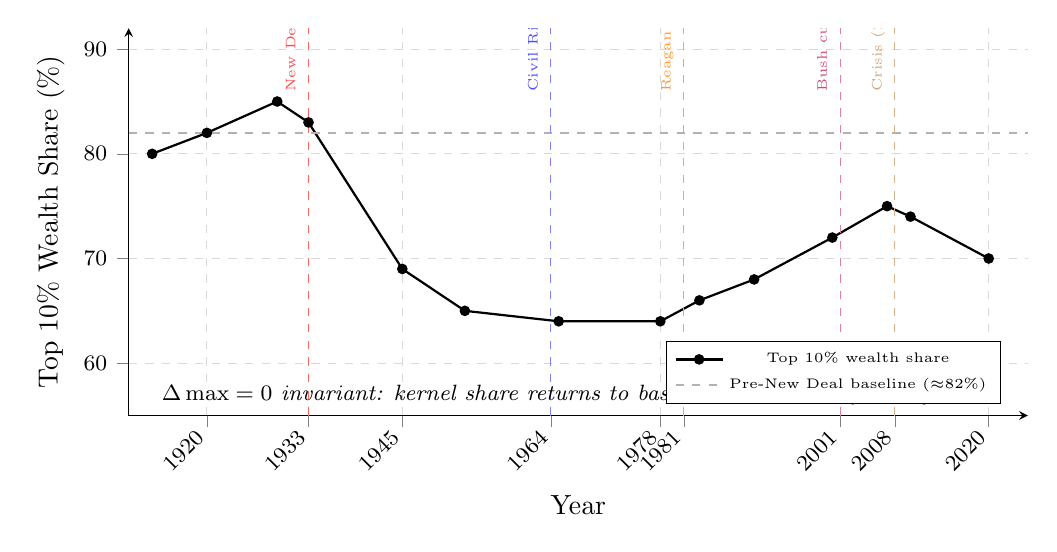
\begin{tikzpicture}
\begin{axis}[
    width=13cm, height=6.5cm,
    xlabel={Year},
    ylabel={Top 10\% Wealth Share (\%)},
    xmin=1910, xmax=2025,
    ymin=55, ymax=92,
    xtick={1920,1933,1945,1964,1978,1981,2001,2008,2020},
    xticklabels={1920,1933,1945,1964,1978,1981,2001,2008,2020},
    x tick label style={rotate=45, anchor=east, font=\footnotesize},
    y tick label style={font=\footnotesize},
    grid=major,
    grid style={dashed, gray!30},
    axis lines=left,
    tick align=outside,
    legend pos=south east,
    legend style={font=\tiny},
]

% Wealth share trajectory (Piketty--Saez--Zucman, WID.world)
\addplot[thick, black, mark=*, mark size=1.5pt] coordinates {
    (1913, 80)
    (1920, 82)
    (1929, 85)
    (1933, 83)
    (1945, 69)
    (1953, 65)
    (1965, 64)
    (1978, 64)
    (1983, 66)
    (1990, 68)
    (2000, 72)
    (2007, 75)
    (2010, 74)
    (2020, 70)
};
\addlegendentry{Top 10\% wealth share}

% Reference band: pre-New Deal baseline (1913--1933 average ~82%)
\addplot[dashed, gray!60, thick] coordinates {(1910,82)(2025,82)};
\addlegendentry{Pre-New Deal baseline ($\approx$82\%)}

% Reform event annotations -- vertical dashed lines
\draw[dashed, red!60, thin] (axis cs:1933,55) -- (axis cs:1933,92);
\draw[dashed, blue!50, thin] (axis cs:1964,55) -- (axis cs:1964,92);
\draw[dashed, orange!70, thin] (axis cs:1981,55) -- (axis cs:1981,92);
\draw[dashed, purple!50, thin] (axis cs:2001,55) -- (axis cs:2001,92);
\draw[dashed, brown!60, thin] (axis cs:2008,55) -- (axis cs:2008,92);

% Event labels at top of figure
\node[rotate=90, anchor=south west, font=\tiny, text=red!70] at (axis cs:1933,85) {New Deal (1933)};
\node[rotate=90, anchor=south west, font=\tiny, text=blue!70] at (axis cs:1964,85) {Civil Rights (1964)};
\node[rotate=90, anchor=south west, font=\tiny, text=orange!80] at (axis cs:1981,85) {Reagan cuts (1981)};
\node[rotate=90, anchor=south west, font=\tiny, text=purple!70] at (axis cs:2001,85) {Bush cuts (2001)};
\node[rotate=90, anchor=south west, font=\tiny, text=brown!70] at (axis cs:2008,85) {Crisis (2008)};

% Delta-max label
\node[anchor=west, font=\footnotesize\itshape, text=black] at (axis cs:1913,57) {$\Delta\max = 0$ invariant: kernel share returns to baseline across all reform cycles};

\end{axis}
\end{tikzpicture}
\caption{\textbf{The $\Delta\max = 0$ Invariant: Top 10\% Wealth Share, 1913--2020.} Despite the New Deal, the Civil Rights Act, environmental and labor legislation, and multiple rounds of progressive tax reform, the Elite's aggregate extraction share---measured as the top decile's portion of total national wealth---returns to near its pre-New Deal baseline by 2020. Each major reform cycle (annotated) produced a temporary downward perturbation, but the closed-loop system re-absorbed every reform and the wealth share resumed its long-run trajectory. This is $\Delta\max = 0$ stated as an empirical time series: the extraction kernel is invariant across every concession in the 1913--2020 dataset. Data from Piketty, Saez, and Zucman (WID.world).}
\label{fig:deltamax_invariant}
\end{figure}

\subsection{The Extraction Engine: Why \texorpdfstring{$\Delta\max = 0$}{Δmax = 0} Is a Legal Mandate}

The Concession Theorem's invariant---$\Delta\max = 0$---has been \textbf{structurally encoded into the legal architecture of the corporation itself}.

Under the doctrine of \textbf{shareholder primacy}, corporate officers bear a fiduciary duty to maximize returns to shareholders. This is the extraction kernel expressed as corporate law: the entity that \textit{directly produces} the capital---the corporation---is \textit{legally obligated} to maximize its extraction rate. A CEO who voluntarily reduces profit margins to improve labor conditions or community welfare risks shareholder derivative suits, hostile board action, and termination. The Predatory Min-Max Function is the \textbf{job description} at the corporate level.

The incentive architecture ensures that the individuals managing the extraction engines are personally fused to the extraction rate. Executive compensation in the modern era is overwhelmingly denominated in \textbf{equity}: stock options, restricted stock units, and performance shares whose value is a direct function of the firm's market capitalization. The CEO's personal wealth \textit{is} the extraction output. Their net worth is $\max$, measured in real time on a ticker. Every structural decision---wage suppression, offshoring, algorithmic labor scheduling, union avoidance---that increases the firm's equity price simultaneously increases the executive's personal fortune. The alignment is total: the human being operating the extraction engine is compensated in units of extraction.

The final architectural layer is the mechanism by which this extracted wealth is \textit{consumed without ever being taxed}. Under the U.S.\ tax code, unrealized capital gains are not income. A CEO whose equity portfolio appreciates by \$500 million in a single year owes \$0 in taxes on that appreciation---because no ``taxable event'' has occurred. To access the wealth for consumption, the executive does not sell the stock (which would trigger capital gains tax and reduce the equity position). Instead, they execute what tax professionals term the \textbf{Buy-Borrow-Die} strategy: they pledge the appreciated stock as collateral and take out low-interest margin loans against it. The loan proceeds are not taxable income. As long as the portfolio appreciates faster than the loan's interest rate---a condition the extraction engine itself is legally mandated to produce---the executive can take out successive loans indefinitely, rolling the balance forward, consuming unlimited liquidity without ever realizing a taxable gain. Upon death, the assets receive a \textbf{stepped-up basis} under IRC \S 1014, resetting the cost basis to the current market value and permanently erasing the unrealized appreciation from the tax base. The heirs inherit the wealth; the treasury receives nothing; the cycle restarts.

This is the mechanical specification of $\Delta\max = 0$. The corporation is legally required to maximize extraction. The executives are compensated in units of extraction. And the tax architecture permits the extracted wealth to be consumed, inherited, and perpetuated without ever passing through the public treasury. No reform that leaves this trilateral architecture intact---fiduciary duty, equity compensation, and the Buy-Borrow-Die loop---can produce $\Delta\max \neq 0$. The constraint is a \textbf{legal machine} that runs whether any individual Elite member wills it or not.

The Concession Theorem predicts that the policy prescriptions identified in this chapter---algorithmic audits, intersection reduction, structural monitoring---are \textit{exactly} what the system will offer when $\min$ approaches failure in the current terminal phase. The framework that diagnoses the disease also predicts the palliative the system will administer. Accepting these reforms resets the clock.

\subsection{Algorithmic Load Balancing: Freedom as a Zero-Sum Market}

The clock resets because the system does not concede extraction; it reroutes it. Let $\ell_g(t)$ denote the extraction load assigned to demographic or jurisdictional group $g$ at time $t$. The Elite's target is to maintain the aggregate extraction yield:
\begin{equation}\label{eq:12.2a-load-balancing}
\sum_{g \in G} \ell_g(t) = \mathcal{E}_{\text{total}}(t),
\qquad
\frac{d\mathcal{E}_{\text{total}}}{dt} \geq 0 .
\end{equation}
If a reform reduces the load on one group without altering $\mathcal{E}_{\text{total}}$, the deficit must be assigned somewhere else:
\begin{equation}\label{eq:12.2b-load-transfer}
\Delta \ell_h
=
-\Delta \ell_g
+ \Delta \mathcal{E}_{\text{total}},
\qquad h \neq g .
\end{equation}

This is the mechanical basis of horizontal hostility. The system pitches groups against each other because each partial concession is experienced by another group as a new burden, a lost status wage, a price increase, a tax shock, a policing surge, or a moral panic. The market being rationed is freedom itself. One population receives a partial autonomy patch; another population is made to pay for it through deeper extraction or diminished access. The resulting conflict is then misread as cultural antagonism when it is load balancing by the extraction kernel.

\subsection{The Acemoglu Limit: Why ``Inclusive Institutions'' Cannot Recompile Without Dismantling the Racial Partition}
\label{sec:acemoglu_limit}

Acemoglu and Robinson's \textit{Why Nations Fail} is the most influential contemporary articulation of the institutional-economics theory of extraction \cite{acemoglu_robinson}. Their core argument---that the divergence between prosperous and impoverished nations reduces to the distinction between ``inclusive'' and ``extractive'' institutions, with the latter concentrating political and economic power at the apex and blocking the creative destruction required for long-run growth---correctly identifies the architecture this book has traced for five centuries. Their comparative historical dataset, their identification of ``critical junctures'' at which institutional divergence becomes self-reinforcing, and their analysis of elite capture of political institutions all converge with the framework developed here at the level of description.

The Acemoglu Limit is the point at which their prescription fails. AJR's solution is the construction of ``inclusive institutions''---pluralist political systems, property rights enforced for all citizens, and competitive markets constrained by centralized state authority. The prescription is that if a nation can complete the transition from extractive to inclusive, the self-reinforcing logic of inclusive institutions will stabilize the outcome. The problem is that this prescription contains no variable for the racial partition, no term for the psychological wage ($\psi$), and no mechanism for the kinetic-guarantee asymmetry. It treats elite capture as a problem of institutional design that can be solved by institutional redesign---by building better rules.

The Concession Theorem falsifies this prescription at every historical juncture. The arc from Reconstruction to the Compromise of 1877 is the purest laboratory case: the United States briefly constructed inclusive institutions during Reconstruction---multiracial legislatures, universal public education, federal civil rights enforcement---and the extraction Elite dismantled them within twelve years by operating through the institutional rules. The ``inclusive institutions'' were recompiled into extractive ones because the Elite retained three variables that AJR's model cannot account for. First, the psychological wage ($\psi$) caused $I_{\text{buffer}}$ to defect from the cross-racial coalition in exchange for racial status, supplying the political mass needed to legitimize the Redeemer counter-revolution. Second, the racial partition ($I_{\text{buffer}}$ vs.\ $O_{\text{racialized}}$) ensured that the Out-group's democratic gains were politically isolable---the Reconstruction coalition could be severed along the racial seam the Elite had installed in 1705. Third, the kinetic-guarantee asymmetry meant that when federal enforcement was withdrawn, the paramilitary enforcement class ($F_{\text{enforce}}$) could impose Redeemer rule through violence that the disarmed Out-group could not match.

Formally, AJR's model is a special case of the Concession Theorem with $\psi = 0$ and no racial partition installed. In a system where the Elite have not successfully deployed a psychological wage to purchase buffer-class complicity, institutional reform can achieve durable equilibrium because the reforming coalition cannot be ethnically fragmented. The American case---and, as Chapter~\ref{ch:global} demonstrates, the global colonial system---is not that special case. The racial partition is installed. $\psi$ is operative. The kinetic asymmetry is legally maintained. Under these conditions, building ``inclusive institutions'' without first dismantling the extraction kernel's three-variable architecture does not produce inclusive equilibrium; it produces Reconstruction---a brief inclusive episode followed by violent counter-revolution and kernel restoration.

AJR's model identifies the causes of national failure accurately; it lacks the variables required to write the patch. \textit{Why Nations Fail} diagnoses the disease with considerable precision; it cannot specify the cure because the cure requires the full five-tier framework---including the psychological-wage mechanism, the racial-partition dynamics, and the kinetic-guarantee architecture---that this book has developed. Inclusive institutions are a necessary condition of the post-kinetic republic; they are not sufficient without simultaneous dismantling of the partition that causes inclusive reforms to recompile back into extraction.

\subsubsection{The Non-Atlantic Objection: Botswana, South Korea, and the Reversal of Fortune}

A critic familiar with the breadth of AJR's empirical work will raise the following objection: the Acemoglu Limit is argued here exclusively through Atlantic cases (Reconstruction, the American dataset). But AJR's empirical program extends far beyond the Atlantic. Their 2002 paper ``Reversal of Fortune'' \cite{ajr_reversal} (Acemoglu, Johnson, and Robinson) documents a striking pattern across former European colonies: societies that were \textit{more} urbanized and densely populated before colonization---and thus, by most pre-modern indicators, more institutionally sophisticated---became \textit{less} developed after colonization, while less-developed pre-colonial territories eventually surpassed them. AJR explain this reversal through the \textit{settler mortality} hypothesis: where European settlers could survive (low disease burden), they built inclusive settler institutions; where they could not, they built pure extraction colonies designed to export resources to the metropole. In their framework, Botswana and South Korea represent cases where either post-independence institutional design or Cold War client-state investment produced inclusive-institution trajectories that broke from the colonial extraction pattern.

The Acemoglu Limit accepts the Reversal of Fortune's empirical findings \cite{ajr_reversal} and contests the model's sufficiency as a patch specification. Three observations show that the AJR dataset is consistent with---and in some respects confirms---the racial-partition model:

\textbf{1. The Reversal of Fortune is the racial partition at global scale.} AJR's settler mortality hypothesis identifies the \textit{mechanism of installation}: where mortality was low enough to permit European settlement, the full five-tier hierarchy was installed---$E$ (settler capital), $P_{\text{uppet}}$ (colonial administration), $F_{\text{enforce}}$ (military), $I_{\text{buffer}}$ (settler working class granted racial status wages), and $O_{\text{racialized}}$ (indigenous and imported labor). Where mortality was too high for settler colonization, extraction colonies were established without the buffer-class partition---pure $E$-$F_{\text{enforce}}$-$O$ structures. The reversal AJR document is, in the framework's vocabulary, the difference between a system with an installed $\psi$ mechanism (settler colonies, which produce durable extractive equilibrium) and one without (extraction-only colonies, which are unstable but extractable at high intensity). AJR correctly identify the correlation between settler mortality and long-run institutional outcomes \cite{ajr_reversal}; the racial-partition model explains the \textit{mechanism}.

\textbf{2. Botswana: the exception that confirms the scope condition.} Botswana is AJR's strongest success case---a former British protectorate that achieved upper-middle-income status through diamond revenues and is routinely cited as evidence that inclusive institution-building can overcome colonial origins. The framework's analysis is precise: Botswana's diamond extraction economy required \textit{skilled} local labor and technical cooperation that the colonial model could not supply through pure coercion. Because the extraction technology demanded a skilled indigenous workforce, the Elite's rational strategy was to invest in $I_{\text{buffer}}$-style material wages for the skilled labor class while avoiding a full racial partition. $\psi$ was deployed as a technocratic material wage to a narrow skilled class; no psychological-wage partition between ethnic groups within a settler society was installed. The result is consistent with the Concession Theorem at smaller scale: Botswana's gains are real, but Gini coefficients remain among Africa's highest, the diamond revenue is concentrated in a narrow elite, and $\Delta\max$ at the apex is structurally intact. AJR use Botswana to demonstrate that institutions can improve; the framework uses it to demonstrate that $\Delta\max = 0$ survives even the most favorable post-colonial cases.

\textbf{3. South Korea: inter-national versus intra-national partition.} South Korea's developmental trajectory---from Japanese colonial extraction to US Cold War client-state to upper-income economy---is a genuine case where AJR's inclusive-institution logic has traction. The framework's explanation is the scope condition: South Korea's colonial experience was \textit{inter-national}. Japanese colonialism extracted from Korea as a national unit; it did not install a permanent intra-Korean racial partition with a $\psi$-stabilized buffer class. When Japanese colonialism ended in 1945, there was no $I_{\text{buffer}}$ class with a psychological investment in the partition's maintenance to fracture the post-independence coalition. The Korean working class and the Korean state could construct the developmental coalition that AJR's model predicts---because there was no ethnic seam for the Elite to exploit. The scope condition holds: the Acemoglu Limit applies specifically to systems where an intra-national racial partition has been installed with an operative $\psi$ mechanism. Where that partition is absent---whether because the colonial form was inter-national or because no buffer-class psychological wage was deployed---AJR's inclusive-institution prescription can achieve the equilibrium they describe.

The Acemoglu Limit is therefore a \textbf{scope condition} of AJR's empirical project: AJR's inclusive-institution prescription succeeds precisely where the framework predicts it should---in systems where $\psi = 0$ and no intra-national racial partition exists. The American case, and the global colonial cases with installed settler buffer classes, are outside this scope. The prescription fails because it was designed for, and validated on, the cases where the missing variables are absent.

\begin{figure}[htbp]
\centering
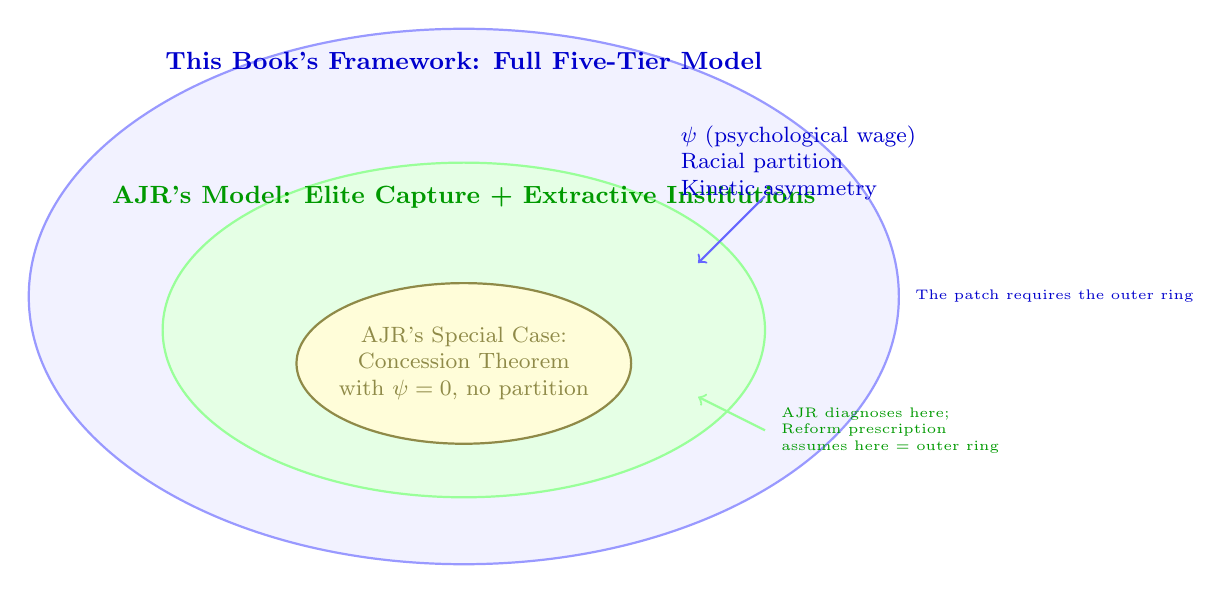
\begin{tikzpicture}[scale=0.85]
    % Outer ellipse
    \draw[thick, fill=blue!5, draw=blue!40] (0,0) ellipse (6.5cm and 4cm);
    \node[anchor=north, font=\small\bfseries, text=blue!80!black] at (0,3.8) {This Book's Framework: Full Five-Tier Model};
    
    % Middle ellipse
    \draw[thick, fill=green!10, draw=green!40] (0,-0.5) ellipse (4.5cm and 2.5cm);
    \node[anchor=north, font=\small\bfseries, text=green!60!black] at (0,1.8) {AJR's Model: Elite Capture + Extractive Institutions};
    
    % Inner ellipse
    \draw[thick, fill=yellow!15, draw=yellow!50!black] (0,-1) ellipse (2.5cm and 1.2cm);
    \node[anchor=center, font=\footnotesize, text=yellow!50!black, align=center] at (0,-1) {AJR's Special Case:\\Concession Theorem\\with $\psi=0$, no partition};

    % Variables labels
    \node[font=\footnotesize, text=blue!80!black, align=left] at (5,2) {$\psi$ (psychological wage)\\Racial partition\\Kinetic asymmetry};
    \draw[->, blue!60, thick] (4.5,1.5) -- (3.5,0.5);

    % Note labels
    \node[anchor=west, font=\tiny, text=blue!80!black] at (6.6,0) {The patch requires the outer ring};
    \node[anchor=west, font=\tiny, text=green!60!black, align=left] at (4.6,-2) {AJR diagnoses here;\\Reform prescription\\assumes here = outer ring};
    \draw[->, green!40, thick] (4.5,-2) -- (3.5,-1.5);

\end{tikzpicture}
\caption{\textbf{The Acemoglu Limit: Model Subset Comparison.} The institutional economics model of Acemoglu and Robinson (middle ring) correctly identifies the extractive/inclusive binary but lacks the variables required to sustain the transition in a racialized system. Their model is a special case (inner ring) where the psychological wage and racial partition are absent. Durable inclusive institutions require the full five-tier model (outer ring) to dismantle the mechanisms that otherwise cause reforms to recompile into extraction.}
\label{fig:acemoglu_limit_venn}
\end{figure}

\section{The Constitutional Shield: The Intent Standard as Concealment Apparatus}

The Concession Theorem demonstrates that the system absorbs reform at the policy level. This section demonstrates that the judiciary provides a parallel shield at the constitutional level through a jurisprudential architecture that is \textit{structurally blind} to the exact form of racial targeting the political establishment has openly admitted to deploying.

Define the judiciary's detection function for racial discrimination as:
\begin{equation}\label{eq:12.3-judiciary-discrimination-detection}
D(P) = \begin{cases}
1 & \text{if } P \text{ explicitly invokes racial classification} \\
0 & \text{if } P \text{ uses proxy variable } x \text{ where } \operatorname{Corr}(x, \text{race}) \to 1
\end{cases}
\end{equation}

The intent standard detects $P$ when and only when $P$ names race directly.\footnote{This equation is classified as Tier~3 (ordinal/structural); the structural detection function is validated by \textit{Washington v.\ Davis} (1976) and \textit{McCleskey v.\ Kemp} (1987), in which the Supreme Court ruled that statistically documented racial disparities are constitutionally insufficient absent proof of discriminatory intent---confirming that $D(P_{\text{proxy}}) = 0$ is the operative judicial standard. See the Empirical Methodology chapter (p.~\pageref{ch:empirical_methodology}) and Appendix~\ref{app:empirical_index}.} But the entire modern apparatus of racial governance---documented in every preceding chapter---operates through proxy variables: ``blight removal,'' ``states' rights,'' ``tax cuts,'' ``law and order,'' ``urban renewal.'' The proxy and the target are statistically identical ($\operatorname{Corr}(x, \text{race}) \to 1$), but the detection function returns 0. This is a \textbf{feature} of the concealment apparatus.

\subsection{The Insurmountable Burden of ``Discriminatory Intent''}

Under the Equal Protection Clause of the Fourteenth Amendment, a government action is not unconstitutional simply because it produces a severe, racially disproportionate impact. Following the Supreme Court's landmark decisions in \textit{Washington v.\ Davis} (1976) and \textit{Village of Arlington Heights v.\ Metropolitan Housing Development Corp.}\ (1977), plaintiffs must prove that the state action was explicitly motivated by ``discriminatory intent'' or racial animus \cite{tel_wash_v_davis, tel_arlington_heights}.

Justice White, writing for the \textit{Washington v.\ Davis} majority, stated the rule unambiguously: ``[O]ur cases have not embraced the proposition that a law or other official act, without regard to whether it reflects a racially discriminatory purpose, is unconstitutional solely because it has a racially disproportionate impact.'' \textit{Washington v.\ Davis}, 426 U.S.\ 229, 239 (1976). Justice Brennan's dissent identified what this rule immunized: a recruitment test for the D.C.\ Metropolitan Police Department that excluded Black candidates at four times the rate of white candidates, with no demonstrated relationship to job performance---precisely the proxy-variable substitution the framework formalizes as $P_{\text{proxy}}$.\footnote{Brennan, J., dissenting, \textit{Washington v.\ Davis}, 426 U.S.\ 229, 263--264 (1976) (``[T]he Court does not explain how it would distinguish between laws that discriminate racially and those that merely have a racially disproportionate impact.''). The dissent's structural argument anticipates Siegel's ``preservation through transformation'' \cite{tel_siegel}: if disparate impact cannot trigger Equal Protection scrutiny, the constitutional guarantee protects only against racial discrimination that is sufficiently \textit{unsophisticated} to announce itself. Sophisticated proxy substitution receives complete immunity.}

The Court in \textit{Arlington Heights} outlined a framework of circumstantial evidentiary factors: (1) disproportionate impact, (2) historical background, (3) sequence of events and departures from normal procedural sequences, (4) legislative or administrative history, and (5) testimony of legislators or decision-makers \cite{tel_arlington_heights}.\footnote{\textit{Village of Arlington Heights v.\ Metropolitan Housing Dev.\ Corp.}, 429 U.S.\ 252, 266--268 (1977). The fifth factor---direct testimony from decision-makers---is the doctrinal tell: courts applying this standard in good faith have all the tools they need to find discriminatory intent in most well-documented racial-disparity cases. The reason they rarely do so is that applying the factors faithfully would void a substantial fraction of mid-century urban planning, transportation, and zoning decisions. The doctrine is structurally designed to produce restraint.} In theory, this allows circumstantial cases. In practice, the federal courts have applied this standard so rigidly that it effectively requires a ``smoking gun''---a memo, a recorded statement, or an overt admission that a highway was routed through a Black community specifically \textit{because of} racial hatred.

Because mid-century urban planners, highway engineers, and politicians were highly adept at laundering racial motivations through race-neutral language---``traffic efficiency,'' ``urban renewal,'' ``blight removal''---such smoking guns rarely exist. The intent standard effectively limits the Fourteenth Amendment to policing overt, individual acts of malice, rendering the Constitution entirely blind to structural, systemic racism.

Applied to the infrastructure documented in the preceding sections:

\begin{table}[htbp]
\centering
\small
\renewcommand{\arraystretch}{1.4}
\begin{tabular}{>{\raggedright}p{5.5cm} >{\raggedright\arraybackslash}p{7.5cm}}
\toprule
\textbf{\textit{Arlington Heights} Factor} & \textbf{Application to Highway Routing} \\
\midrule
\textbf{Disproportionate Impact} & Clear: highways disproportionately displaced Black residents and concentrated vehicular pollution on $O_{\text{racialized}}$. (Legally insufficient alone.) \\
\textbf{Historical Background} & Redlining preceded highway placement, artificially depressing land values to justify ``slum clearance.'' (Deemed ``too remote.'') \\
\textbf{Procedural Departures} & Planners canceled public hearings in Black neighborhoods (Overtown, Miami) or ignored routing criteria favoring intact neighborhoods. (``Administrative discretion.'') \\
\textbf{Contemporary Statements} & Extremely rare. When they exist (Miami planners citing ``continued whiteness of central Miami''), courts still struggle to apply structural remedies. \\
\bottomrule
\end{tabular}
\caption{\textbf{The \textit{Arlington Heights} Framework Applied to $\Sigma_{\text{highway}}$.} Each evidentiary factor is either legally insufficient standing alone or functionally unobtainable, creating a hermetically sealed legal shield for structurally racist state action.}
\label{tab:arlington_heights}
\end{table}

\subsection{The Atwater Proof: The Proxy Variable as Deliberate Encoding}

The intent standard's fatal deficiency is that it was \textit{designed to be satisfied only by the crude, obsolete forms of racism that the political establishment had already abandoned}. The most devastating proof comes from the architects of the strategy themselves.

Lee Atwater's 1981 confession, quoted in full in Section~3.3, constitutes a frank admission of deliberate variable substitution: the explicit racial variable (direct invocation of racial slurs) became politically costly, so the apparatus replaced it with \textbf{proxy variables}---``forced busing,'' ``states' rights,'' ``tax cuts,'' ``law and order.'' The function remained identical: the input is racial targeting, the output is racially concentrated harm. The variable names were obfuscated to evade detection. Atwater himself notes that the racial harm is a known ``byproduct''; the abstraction is a deliberate concealment strategy that preserves the objective.

Formally, let $P_{\text{explicit}}$ denote a policy that names race directly, and $P_{\text{proxy}}$ denote a policy targeting proxy variable $x$ where $\operatorname{Corr}(x, \text{race}) \to 1$. Then:
\begin{equation}\label{eq:12.4-proxy-discrimination-equivalence}
|O_{\text{racialized}} \cap P_{\text{explicit}}| \approx |O_{\text{racialized}} \cap P_{\text{proxy}}|
\end{equation}
The intersection---the set of people harmed---is identical.\footnote{This equation is classified as Tier~3 (ordinal/structural); the structural equivalence claim is validated by Alexander (2010) showing that the War on Drugs proxy achieves the same racial partition as Jim Crow's explicit targeting, and by Atwater's 1981 direct admission that the proxy substitution was deliberate---the variable names changed but the functional output ($|O_{\text{racialized}} \cap P|$) did not. See the Empirical Methodology chapter (p.~\pageref{ch:empirical_methodology}) and Appendix~\ref{app:empirical_index}.} But the detection function yields $D(P_{\text{explicit}}) = 1$ and $D(P_{\text{proxy}}) = 0$. The \textit{more sophisticated the concealment}, the \textit{more complete the legal immunity}. The intent doctrine \textit{succeeds at protecting} dog-whistle racism.

Legal scholar Charles R.\ Lawrence III identified this structural defect in ``The Id, the Ego, and Equal Protection: Reckoning with Unconscious Racism'' (\textit{Stanford Law Review}, 1987), arguing that the intent doctrine ``immunizes from judicial scrutiny'' all but the most overtly expressed racism \cite{tel_lawrence}. Reva Siegel extended the critique with the concept of ``preservation through transformation''---the observation that discriminatory regimes adapt their justificatory rhetoric to survive legal prohibition while maintaining identical functional outcomes (\textit{Stanford Law Review}, 1997) \cite{tel_siegel}. Ian Haney L\'{o}pez, in \textit{Dog Whistle Politics} (2014), provides the most systematic treatment, demonstrating that terms such as ``welfare queens,'' ``illegal aliens,'' ``inner city crime,'' and ``states' rights'' function as racial code that activates racial resentment while permitting speakers to deny racial intent \cite{lopez}.

\subsection{Judicial Deference and the Formalism of Infrastructure}

When Black communities attempted to halt the destruction of their neighborhoods through litigation, the judiciary consistently deferred to executive prerogative. In \textit{Nashville I-40 Steering Committee v.\ Ellington} (1968), Black plaintiffs presented massive circumstantial evidence that the highway was intentionally rerouted to spare white commercial interests and destroy Black neighborhoods. The Sixth Circuit acknowledged the devastating impact but flatly rejected the constitutional claim: ``In the absence of proof of racial discrimination, we do not consider this matter to be a justiciable issue. The routing of highways is the prerogative of the executive department of government, not the judiciary'' \cite{tel_nashville_case}.

This ruling exposes a secondary barrier: courts have historically struggled to recognize the pouring of concrete as a ``regulatory'' action capable of violating civil rights. By classifying highway routing as a purely technical, administrative choice, the judiciary removed it from constitutional scrutiny and granted planners near-absolute immunity to weaponize infrastructure. Within the framework, this judicial formalism is itself a component of the concealment apparatus: $\Sigma_{\text{highway}}$ operates in a domain the judiciary categorically refuses to scrutinize.

\subsection{The Evisceration of Title VI: Closing the Last Pathway}

Recognizing the Fourteenth Amendment's limitations, racial justice advocates attempted to use Title VI of the Civil Rights Act of 1964. Section 602 authorized federal agencies like the EPA and DOT to promulgate regulations forbidding actions with ``disparate impact''---allowing plaintiffs to challenge environmental racism \textit{without} needing to prove intent \cite{tel_title_vi}.

This pathway was destroyed in 2001. In \textit{Alexander v.\ Sandoval}, the Supreme Court ruled that private citizens do \textbf{not} possess a private right of action to enforce Title VI disparate impact regulations \cite{tel_sandoval}. Following \textit{Sandoval}, only federal agencies have enforcement authority, leaving vulnerable communities entirely at the mercy of executive branch political will and resource constraints.

\paragraph{Primary statutory text (Title~VI, \S2000d).}
The operative Title~VI sentence appears at \usclink{apx:usc:42:2000d}{42 U.S.C.~\S~2000d}:
\uscinline{usc_42_2000d}

The result is a hermetically sealed legal architecture:
\begin{itemize}
\tightlist
\item The \textbf{Equal Protection Clause} requires intent $\rightarrow$ intent is unprovable when the system operates through proxy variables $\rightarrow$ $D(P_{\text{proxy}}) = 0$.
\item \textbf{Title VI disparate impact} could detect proxy variables $\rightarrow$ private enforcement eliminated by \textit{Sandoval} $\rightarrow$ pathway closed.
\item \textbf{Judicial formalism} classifies infrastructure as ``administrative'' $\rightarrow$ $\Sigma_{\text{highway}}$ escapes scrutiny entirely.
\end{itemize}

Communities suffering from the generational, compounding toxicity of mid-century highway placement---communities whose children were poisoned by $P_{\text{lead}}$ concentrated by $\Sigma_{\text{highway}}$ within $P_{\text{redlining}}$---exist in a state of permanent legal limbo. The Constitution cannot see what the algorithm does, because the algorithm was designed to operate below the Constitution's detection threshold. The intent standard does not \textit{fail} to detect the extraction kernel; it \textit{immunizes} it. Atwater confessed the substitution. The math confirms it. The law refuses to read what has already been written.

\section{The Judicial Node: Double-Agent Architecture}

The contrast between civil-rights formalism and Second Amendment doctrine reveals that the judicial node is not incapable of systemic analysis. It is selectively routed. Define the judicial node as $P_{\text{jud}}$, a compiler that chooses between two detection modes:
\begin{equation}\label{eq:12.4a-judicial-double-agent}
P_{\text{jud}}(P)=
\begin{cases}
D_{\text{sem}}(P_{\text{proxy}})=0 & \text{software-layer civil-rights and voting claims},\\
D_{\text{hist}}(P_{\text{kinetic}})>0 & \text{hardware-layer Second Amendment claims}.
\end{cases}
\end{equation}

This compiler operates as a measurable structural mechanism. Judicial-politics research now treats judicial language and expert-observed judging behavior as measurable traces of latent ideology. Truscott and Romano show that Supreme Court opinion text can recover ideological structure from lexical variation, while Cope's JuDJIS project shows that expert descriptions of federal judges can be scaled into dynamic ideology measures that outperform common political proxies in predicting appellate behavior \cite{truscott_romano_judicial_text_2026,cope_judjis_2025}. In this book's vocabulary, $P_{\text{jud}}$ has measurable preference weights. That does not prove bad faith by any particular Justice; it means the judicial node leaves semantic fingerprints when it chooses which priors to load.

In the civil-rights register, the Court's interface is formal symmetry. \textit{Ames v.\ Ohio Department of Youth Services} rejected a heightened ``background circumstances'' rule for majority-group Title VII plaintiffs, compiling the civil-rights statute as an individual, direction-agnostic command detached from remedial architecture keyed to historical subordination \cite{ames_ohio_dys_2025}. In \textit{Louisiana v.\ Callais}, the Court treated race-conscious Voting Rights Act districting pressure as an equal-protection collision, while Justice Thomas's concurrence would disable Section~2 districting claims more categorically \cite{louisiana_v_callais_2026}. The effect is the same compiler behavior this chapter has already formalized: if the proxy does not name race directly, $D(P_{\text{proxy}})=0$; if a remedial tool names race to counteract historical extraction, the colorblind interface reclassifies the remedy itself as the constitutional injury.

In \textit{Bruen}, Justice Thomas does the opposite. The semantic interface is powered down and historical due diligence is powered up. New York's ``proper cause'' requirement is treated as a subjective bottleneck on the kinetic guarantee, not as a neutral administrative filter entitled to deference. The Court asks who had discretion, where the discretion came from, what tradition can justify it, and whether the state has carried the burden. That is precisely the analysis the civil-rights cases refuse to perform when the proxy variable is zoning, highway routing, criminality, district shape, testing, or administrative discretion.

The observation concerns capacity: the legal node can see systemic oppression when the threatened variable is hardware-level kinetic parity. It can identify administrative discretion as a constitutional danger, reject interest balancing, and force the state to justify its proxy against history. The same node powers down that capability when the threatened variable is software-level political extraction. The double-agent architecture is therefore visible: semantic formalism protects the extraction kernel in civil-rights and voting cases; kinetic due diligence protects the hardware channel that the constitutional order cannot openly admit it is still rationing by class and race.

\subsection{Case Study: Judicial Semantic Priors in the SCOTUS Corpus}

The claim above can be tested against the book's local SCOTUS corpus as a language problem. Recent judicial-politics work justifies this move. Truscott and Romano adapt Wordshoal to Supreme Court opinion text and show that lexical variation in opinions can recover latent ideological structure strongly correlated with Martin--Quinn scores \cite{truscott_romano_judicial_text_2026}. Cope's JuDJIS project reaches the same methodological premise from the opposite direction: expert descriptions of judging can be transformed into quantitative judicial-ideology measures, and those measures outperform common political proxies in predicting appellate votes \cite{cope_judjis_2025}. The study here does not reproduce either method. It uses their shared premise more narrowly: judicial language is observable behavior, and therefore can be scored as evidence of the semantic prior being compiled.

The workflow in \texttt{Paper/scripts/scotus\_judicial\_semantics.py} reads the expanded markdown case corpus in \texttt{Paper/research/markdown\_cases/}, links each file to \texttt{case\_index.yaml}, strips OCR boilerplate, and attempts majority/concurrence/dissent splits when the text contains reliable opinion markers. It then computes anchored semantic baskets for structural-context language, formalist/procedure language, intent-doctrine language, historical-tradition language, kinetic-rights language, and remedy-narrowing language. A latent text axis is derived from the corpus with a simple SVD over normalized term frequencies and oriented so higher values represent the historical/kinetic pole. The result is a case-level semantic study.

The current run loads 101 indexed cases and produces 190 scored text units, including opinion-unit splits for 49 cases. At the case level, the civil-rights/voting cluster set averages \(-0.53\) on the oriented latent axis, while the Second Amendment cluster averages \(+0.79\). The expert-coded validation sample also separates in the expected direction on the anchored basket delta: \textit{Washington v.\ Davis}, \textit{Arlington Heights}, \textit{Mobile v.\ Bolden}, \textit{McCleskey}, \textit{Shelby County}, \textit{Brnovich}, \textit{Parents Involved}, and \textit{Students for Fair Admissions} fall on the formalist/proxy-screen pole; \textit{Heller}, \textit{McDonald}, \textit{Caetano}, \textit{Bruen}, and \textit{Rahimi} fall on the historical/kinetic pole. The finding is exploratory, because several case files contain records and briefs as well as opinions, and because the unit of analysis is the case, not the Justice. The direction is exactly what Equation~\ref{eq:12.4a-judicial-double-agent} predicts: the Court's language changes when the protected object changes.

\IfFileExists{figures/spectral/scotus_civil_rights_vs_second_amendment.pdf}{%
\begin{figure}[H]
\centering
\includegraphics[width=0.82\linewidth]{figures/spectral/scotus_civil_rights_vs_second_amendment.pdf}
\caption{Case-level semantic-axis comparison between civil-rights/voting cases and Second Amendment cases in the local SCOTUS markdown corpus. Higher values indicate the historical/kinetic pole; lower values indicate the formalist/proxy-screen pole.}
\label{fig:scotus_judicial_semantics_group}
\end{figure}
}{}

The result matters for the fractal mind-virus frame because courts distribute executable interpretive priors. In civil-rights and voting cases, the prior teaches the host population to experience structural extraction as neutral procedure: burden, intent, standing, facial neutrality, administrative normality, and remedy limits. In the Second Amendment cases, the same institution teaches a different prior: history, tradition, text, arms, self-defense, and state burden. The judicial node is a semantic compiler that selectively loads different priors into public cognition. That is why $P_{\text{jud}}$ functions as a double agent: it can perform deep structural due diligence, but it reserves that capacity for the hardware channel while letting software-level racial extraction run below the detection threshold.

\section{The Bruen Load-Balancing Proof}

The Supreme Court's decision in \textit{New York State Rifle \& Pistol Association, Inc.\ v.\ Bruen} (2022) provides a pristine instantiation of the Concession Theorem operating in real time---and reveals the deeper mechanism by which the Elite permits apparent concessions while preserving the kernel.

Justice Thomas's majority opinion contained two declarations that, taken at face value, should have demolished the entire disarmament architecture. First, quoting \textit{McDonald}: the Second Amendment right ``is not `a second-class right, subject to an entirely different body of rules than the other Bill of Rights guarantees.' '' Second, Thomas established that the Second Amendment ``is the very product of an interest balancing by the people,'' and that it ``surely elevates above all other interests the right of law-abiding, responsible citizens to use arms'' for self-defense---explicitly rejecting the means-end scrutiny that lower courts had used for a decade to rubber-stamp every gun control law that reached their dockets. Thomas replaced it with a text-history-and-tradition test: if the government wants to restrict the right, it must demonstrate that the restriction ``is consistent with the Nation's historical tradition of firearm regulation.'' \textit{NYSRPA v.\ Bruen}, 597 U.S.\ 1, 17 (2022) (Thomas, J.).\footnote{Thomas articulated the terminal test as follows: ``[W]hen the Second Amendment's plain text covers an individual's conduct, the Constitution presumptively protects that conduct. The government must then justify its regulation by demonstrating that it is consistent with the Nation's historical tradition of firearm regulation.'' \textit{Bruen}, 597 U.S.\ at 24. The phrase ``plain text covers'' is the entry gate; the phrase ``historical tradition'' is the substantive test. The framework predicts that the ``responsible, law-abiding citizen'' qualifier embedded in Thomas's framing functions as a proxy variable: it is the doctrinal mechanism by which prior criminal-justice contact---disproportionately distributed across $O_{\text{racialized}}$---is laundered into a constitutional exclusion without requiring explicit racial enumeration.} No more interest-balancing. No more deference to legislative judgment. The Constitution already balanced the interests; the legislature does not get to rebalance them.

On its face, \textit{Bruen} was a nuclear event for the disarmament architecture. Thomas struck down New York's subjective ``proper cause'' licensing requirement---the same Sullivan Law template from 1911 that had functioned as the primary filter for asymmetric disarmament for over a century. The ruling appeared to be a genuine concession: the Supreme Court, acting as the judicial layer of $P_{\text{uppet}}$, seemingly expanded constitutional autonomy for the Out-group and Buffer Class.

The system's response reveals \textit{Bruen} as algorithmic load-balancing that preserves the extraction kernel. The Elite permits the ruling because the state-level implementation preserves the extraction kernel through two parallel execution paths:

\begin{itemize}
    \item \textbf{Blue-state path:} Democratic legislatures immediately legislate the ruling into functional nonexistence. By aggressively expanding ``Sensitive Places'' ($P_{\text{spatial}}$), imposing exorbitant licensing fees, mandating insurance requirements, and constructing bureaucratic felony traps, these states achieve the \textit{same mathematical output} as the struck-down ``proper cause'' regime---asymmetric disarmament of $O$ and $I_{\text{buffer}}$---while feeding new bodies into the carceral engine through spatial criminalization.

    \item \textbf{Red-state path:} Republican legislatures nominally comply with \textit{Bruen} by expanding carry rights, but the Enforcement Class ($F_{\text{enforce}}$) compensates through intensified enforcement and operational reality. The lethal autonomy gap is maintained through the application of force. The structural reality is that for both the Out-group ($O_{\text{racialized}}$) and increasingly the Buffer Class ($I_{\text{buffer}}$), the mere possession of a legal firearm in the presence of an officer is a potentially fatal event.

    This pattern extends beyond the single tragedy of Philando Castile. For the Out-group, the lethality of the kinetic guarantee is demonstrated by Amir Locke (killed in 2022 during a no-knock raid while waking up with his legally owned handgun), Breonna Taylor (killed in Louisville in 2020 during a no-knock raid after her partner fired a legally justified warning shot at unidentified intruders), Jemel Roberson (a Black security guard killed by police in 2018 while actively subduing an active shooter), Roger Fortson (a Black U.S.\ Airman killed in his own apartment in 2024 while holding a legally owned gun pointed down), and most recently Christian Diaz Rendon (a Latino homeowner killed by Phoenix police in 2026 inside his own home immediately after successfully disarming an intruder). For the Buffer Class, the exact same lethal override applies. The most heinous instantiation is Daniel Shaver (a white man killed by Mesa police in 2016, shot while unarmed, crying, and crawling on the floor trying to comply with contradictory commands, after police responded to a report of a pellet gun). The pattern continues with Ryan Whitaker (a white man killed by Phoenix police in 2020 after answering his door with a legally owned gun pointed down, despite immediately kneeling and surrendering the weapon) and Johnny Hurley (a white civilian who stopped an active shooter in Colorado in 2021, only to be killed by responding police who saw him holding a weapon).

    $F_{\text{enforce}}$ treats the civilian exercise of the kinetic guarantee as an immediate, shootable threat, overriding the statutory right entirely. This dynamic is a universal feature of the policing architecture in both red and blue jurisdictions, not confined to red states or limited to the Out-group. The legal right to bear arms is instantly nullified by $F_{\text{enforce}}$'s demand for absolute physical dominance during any encounter.
\end{itemize}

Either path preserves the kernel. \textit{Bruen} functions as the system distributing its extraction load across two parallel processors. The ruling reduces $\min$ (the Buffer Class feels its ``rights'' are being defended) without altering $\max$ (the Elite's monopoly on violence remains structurally guaranteed through $F_{\text{enforce}}$ and the statutory immunity documented in Section~6.7.4).

\subsection{The Alito Concurrence: Who Needs the Kinetic Guarantee Most}

Justice Alito's concurring opinion in \textit{Bruen} inadvertently provides the framework's own argument from the mouth of a Supreme Court Justice. Alito directly confronted the dissent's statistical barrage with a single question: \textit{who actually needs the right to carry a firearm for self-defense?}

\begin{quote}
``No one apparently knows how many of the 400 million privately held guns are in the hands of criminals, but there can be little doubt that many muggers and rapists are armed and are undeterred by the Sullivan Law. \ldots Some of these people live in high-crime neighborhoods. Some must traverse dark and dangerous streets in order to reach their homes after work or other evening activities. Some are members of groups whose members feel especially vulnerable. And some of these people reasonably believe that unless they can brandish or, if necessary, use a handgun in the case of attack, they may be murdered, raped, or suffer some other serious injury.'' \cite{bruen}
\end{quote}

Alito does not name the Out-group. He does not have to. ``High-crime neighborhoods,'' ``dark and dangerous streets,'' ``members of groups whose members feel especially vulnerable''---this is the spatial and demographic profile of $O_{\text{racialized}}$ described in the clinical language of judicial opinion. The people most endangered by the Sullivan Law's discretionary denial of lethal autonomy are the same people the Sullivan Law was designed to disarm in 1911.

The \textit{amicus} briefs filed in the case make the subtext explicit. Briefs were submitted by Black Guns Matter, the National African American Gun Association, the Asian Pacific American Gun Owners Association, the Independent Women's Law Center, the DC Project Foundation, and Black Attorneys of Legal Aid---each representing populations that the disarmament architecture has historically targeted. The Brief for Black Attorneys of Legal Aid recounted incidents in which law-abiding citizens were ``driven to violate the Sullivan Law because of fear of victimization'' and were then ``arrested, prosecuted, and incarcerated'' \cite{bruen}. The system criminalized the Out-group for attempting to acquire the kinetic guarantee, then cited the resulting criminalization as justification for further disarmament.

Alito also surfaced the oral argument exchange that distills the discretionary regime to its essence. New York's solicitor general was asked about ``an ordinary person who works at night and must walk through dark and crime-infested streets to get home''---a person who pleads: ``There have been a lot of muggings in this area, and I am scared to death.'' The solicitor general's candid answer was ``in general,'' no---such a person would not be issued a carry permit under New York's ``proper cause'' standard \cite{bruen}. The state acknowledged, under oath, that the licensing regime was designed to deny the kinetic guarantee to ordinary citizens who face lethal threats. This is the designed feature of the Sullivan Law framework. The system denies lethal autonomy to the people who need it most, then deploys $F_{\text{enforce}}$---which has no constitutional duty to protect them (DeShaney, Castle Rock)---as the exclusive and insufficient substitute.

\subsection{The Breyer Silence: What the Dissent Cannot Say}

Justice Breyer's dissent completes the proof through omission. Breyer opens with eight pages of gun violence statistics---45,222 Americans killed by firearms in 2020, 277 mass shootings in the first half of 2022, gun violence as the leading cause of death among children. He then offers a single sentence that, read through the framework, is the most revealing admission in the entire case:

\begin{quote}
``And the consequences of gun violence are borne disproportionately by communities of color, and Black communities in particular. \ldots 34.9 firearm-related homicides per 100,000 population for non-Hispanic Black men in 2019, compared to 7.7 such homicides per 100,000 population for men of all races.'' \cite{bruen}
\end{quote}

Breyer deploys this statistic to argue \textit{for} gun control---to justify the state's ``compelling interest'' in restricting firearms access. He never asks the structurally prior question: \textit{why} are Black communities disproportionately impacted by gun violence? He never connects the 4.5x disparity to the centuries of racialized disarmament, spatial containment, economic extraction, and carceral processing that the framework documents. He cites the \textit{symptom} of the extraction kernel as justification for \textit{deepening} the extraction kernel.

The dissent is equally silent on the \textbf{environmental preprocessing} that the framework treats as $P_{\text{lead}}$ (Chapter~\ref{ch:recompile}). For decades, \textbf{tetraethyllead in motor-vehicle gasoline} dispersed neurotoxic dust along dense urban traffic corridors---overlapping the same redlined geographies where the Out-group had already been concentrated---so that a generation bore disproportionate exposure through the air and soil left by \textit{cars of the past}. That historical channel is only half the story. \textbf{Lead did not end when leaded gas was phased down:} millions of Americans still drink water that passes through \textbf{legacy lead service lines}, and \textbf{schools} remain a major site of exposure when aging pipes, solder, and fixtures leach lead into fountains and cafeterias, with remediation chronically underfunded and unevenly distributed. To name those facts in the same breath as firearm-homicide disparities would invite an obvious question---why the state treats gun violence as a compelling reason to restrict the kinetic guarantee while tolerating, year after year, preventable neurotoxic exposure through public water and public education infrastructure. Breyer's opinion never asks it. The omission preserves the same move as the silence on racialized gun-control history: present lethal violence as a \textit{standalone} public-safety emergency while bracketing the upstream biological and spatial inputs the algorithm already applied.

What Breyer \textit{cannot} say---what no Justice in the majority, concurrence, or dissent says---is what Thomas's own historical evidence proves: that gun control in America has never been racially neutral. Thomas spends pages documenting the Sullivan Law's anti-immigrant origins, the Reconstruction-era disarmament campaigns, Dred Scott's ``parade of horribles,'' the Freedmen's Bureau lieutenant who watched Black men fined for an offence ``committed hourly by every other white man I meet in the streets''---and then treats this evidence as exclusively relevant to the \textit{historical} analysis under the text-history-tradition test. No Justice draws the structural conclusion: that if gun control was a racial operation in 1866, in 1911, in 1967, and in every documented era of American history, then the burden of proof falls on anyone claiming it has somehow stopped being one.

Breyer's silence on the racial history of the law he defends is a structural impossibility. The dissent \textit{cannot} engage with the racial dimension of gun control because doing so would require acknowledging that the Sullivan Law---the very regime Breyer seeks to preserve---was designed to disarm immigrant communities, was enforced asymmetrically against people of color for a century, and that its discretionary framework guaranteed racially disproportionate outcomes by design. A Justice committed to the discretionary licensing model cannot simultaneously acknowledge that discretion has been exercised as a racial weapon for 111 consecutive years. The silence is the argument.

\section{The Grandfather Clause: Gradualist Disarmament and the Boiling Frog}

The Bruen Load-Balancing Proof demonstrates that the system permits apparent concessions while preserving the kernel through parallel execution paths. The \textit{mechanism} by which those blue-state legislative responses actually achieve gradualist disarmament---without triggering the kinetic threshold---requires a closer analysis. The central instrument is the \textbf{grandfather clause}: the single most important tool in the Elite's post-\textit{Bruen} disarmament architecture.

\subsection{The Gradualist Constraint: Why the Elite Cannot Confiscate}

The Elite ($E$) faces a fundamental operational constraint: they \textit{cannot} execute universal disarmament in a single legislative act. The historical record of their own system proves why. The American Revolution---the kinetic action that created the constitutional architecture---was triggered by precisely this scenario. When the British Crown attempted to confiscate colonial firearms at Lexington and Concord in April 1775, the population reached kinetic threshold within hours. The result was a new government.

The Framers encoded this lesson directly into the Second Amendment (Section~8.4), and George Mason articulated the Elite's resulting strategic constraint with mathematical precision: they ``should not do it openly, but weaken them, and let them sink gradually.'' The grandfather clause is the legislative implementation of Mason's warning---the mechanism by which the system achieves disarmament \textit{below the threshold of perceived emergency}, ensuring that the population never experiences the single catalytic moment that would unite $I_{\text{buffer}}$ and $O_{\text{racialized}}$ against $F_{\text{enforce}}$.

The mechanism operates as follows:

\begin{enumerate}
    \item \textbf{Ban new acquisition:} The Puppet Class ($P_{\text{uppet}}$) passes legislation prohibiting the future purchase, manufacture, or transfer of specific categories of firearms---commonly semi-automatic rifles classified as ``assault weapons,'' standard-capacity magazines, or unserialized frames and receivers.

    \item \textbf{Grandfather existing ownership:} The same legislation includes a provision permitting current owners to retain their existing hardware, provided they comply with registration, serialization, or licensing requirements.

    \item \textbf{Asymmetric temporal impact:} Because the ban applies only to \textit{future} acquisitions, the population that already possesses the hardware (predominantly $I_{\text{buffer}}$, who have accumulated multiple firearms over decades) experiences minimal immediate disruption. The population that is \textit{currently acquiring} hardware for the first time---disproportionately $O_{\text{racialized}}$, who are arming at historically unprecedented rates---is immediately locked out of parity.
\end{enumerate}

The grandfather clause is therefore a \textbf{temporal proxy variable} ($P_{\text{grandfather}}$) that achieves racially asymmetric disarmament without ever referencing race. It exploits the historical timeline of the extraction algorithm itself: because the system spent centuries disarming $O_{\text{racialized}}$ through the Black Codes, the Mulford Act, economic filters, and selective enforcement, the Out-group enters the current moment with a massive firearms deficit relative to $I_{\text{buffer}}$. By freezing acquisitions at the current distribution, the grandfather clause \textit{locks in the asymmetry produced by four centuries of racialized disarmament} while presenting itself as a race-neutral public safety measure.

\subsection{The Grandfather Clause as a $\psi_m$ Payment}

The temporal-proxy framing ($P_{\text{grandfather}}$) describes the \textit{structural function} of the grandfather clause. The suppression-allocation framework identifies its \textit{economic logic}. The grandfather clause is a $\psi_m$ payment in the precise technical sense defined in Section~\ref{sec:full_reveal}: $E$ and $P_{\text{uppet}}$ grant $I_{\text{buffer}}$ a material concession---``you keep your rifles''---to secure their political alignment and foreclose their organized opposition to the legislation. The entire cost of that concession is borne exclusively by $O_{\text{racialized}}$, who face felony prosecution for the identical conduct that $I_{\text{buffer}}$ now performs freely under the grandfathered exemption. The invariant $\Delta\max = 0$ holds exactly: the Elite surrenders nothing from their own share; the concession to $I_{\text{buffer}}$ is purchased entirely through the deepened extraction of $O_{\text{racialized}}$'s constitutional rights.

This classification makes the dual-track Second Amendment visible as a formal class-conditional function. The law does not regulate \textit{conduct}; it regulates \textit{class membership}:

\begin{equation}\label{eq:12.11-dualtrack-2a}
\text{Response}(\text{arms},\, x) =
\begin{cases}
\text{constitutionally protected} & x \in I_{\text{buffer}} \\
\text{felony prosecution} & x \in O_{\text{racialized}}
\end{cases}
\end{equation}

The conduct variable is held constant---possession of an identical firearm---while the legal outcome is determined entirely by the actor's position in the five-tier hierarchy. This is a structural equality violation. The same act produces different criminal consequences based on class membership that correlates directly with race.

The compounding model established in Chapter~\ref{ch:full_algo} is the final analytical instrument required. The grandfather clause does not operate on a clean slate; it functions as the terminal multiplicative factor in a documented compounding chain of racial exclusion:

\begin{equation}\label{eq:12.12-grandfather-compound}
B(O_{\text{racialized}}) = \prod_{k} (1 + \delta_k)
\end{equation}

where the compounding layers in the post-\textit{Bruen} disarmament context are:

\begin{itemize}
    \item $\delta_1$: \textbf{Redlining-induced generational wealth gap}---restricts $O_{\text{racialized}}$'s ability to purchase grandfathered hardware at the inflated secondary-market prices that artificial scarcity produces.
    \item $\delta_2$: \textbf{War on Drugs felony exclusions}---disqualifies a disproportionately Black population from lawful firearm ownership entirely under 18~U.S.C.~\S~922(g)(1), before the grandfather clause even applies.
    \item $\delta_3$: \textbf{High-crime-area enforcement concentration}---ensures $F_{\text{enforce}}$ deployment is geographically targeted at $O_{\text{racialized}}$ communities, maximizing the prosecution rate for any technical non-compliance.
    \item $\delta_4$: \textbf{The temporal cutoff itself}---adds felony exposure for the identical conduct that is constitutionally protected for $I_{\text{buffer}}$, as the final multiplicative layer.
\end{itemize}

A policy analysis that treats the grandfather clause as operating in isolation---as a neutral public safety measure with a regrettable statistical skew---systematically understates the constitutional harm by treating $\delta_4$ alone while ignoring the product $\prod_k(1 + \delta_k)$. The law does not \textit{correlate} with prior discrimination; it \textit{multiplies} four centuries of prior discriminatory harm into present constitutional deprivation. No historical tradition cited under \textit{Bruen} can be constitutionally valid if that tradition is itself a compounding sequence of unconstitutional racial exclusions---and the burden the government bears under \textit{Bruen} requires a historical analogue that is both \textit{analogous} and \textit{constitutional}. No such analogue exists for a law that implements a $\psi_m$ payment to $I_{\text{buffer}}$ funded by stripping $O_{\text{racialized}}$ of its constitutional guarantee.

\begin{keyinsight}[Massachusetts Chapter 135: The $\psi_m$ Mechanism Observed in Real Time]
The legislative history of Massachusetts Chapter 135 (2024) provides a rare real-time observation of the $\psi_m$ deployment sequence on the public record, with dates, names, and direct quotes. The timing of the legislation is not incidental. The period 2019--2021 produced a measurable structural shift in the composition of American gun ownership, and the causes of that shift are themselves framework-legible.

Three catalysts converged simultaneously. First, the COVID-19 pandemic and the May 25, 2020 murder of George Floyd by Minneapolis police officer Derek Chauvin generated a rational reassessment of police protection among Black Americans: if $F_{\text{enforce}}$ cannot be relied upon for protection---and may itself be the threat---then the anti-tyranny protocol becomes the operative logic of self-defense \cite{guardian_black_guns_2021}. Second, the Supreme Court's grant of certiorari in \textit{New York State Rifle \& Pistol Association, Inc.\ v.\ Bruen} (April 26, 2021) signaled the imminent abolition of ``may-issue'' discretionary permitting regimes \cite{bruen}. May-issue had functioned for over a century as the administrative mechanism by which $F_{\text{enforce}}$ and local $P_{\text{uppet}}$ disarmed $O_{\text{racialized}}$ under facially neutral law. The canonical example: Dr.\ Martin Luther King Jr.\ applied for a concealed carry permit in Montgomery, Alabama in 1956 after his home was firebombed and he faced documented death threats. The permit was denied at the discretion of local police \cite{mlk_permit_denied, goa_mlk_harvard}. May-issue was the administrative interface through which the dual-track Second Amendment was operationalized. \textit{Bruen}'s decided ruling (June 23, 2022) struck down this discretion and converted may-issue states to shall-issue, removing the gatekeeper mechanism that had kept Black applicants arbitrarily disarmed for generations. Third, these forces combined to produce the statistical signal: NSSF industry surveys identified African American women as the fastest-growing demographic of new gun owners, with an 87\% growth rate; African American firearm purchases rose 58\% in 2020; 60\% of retailers reported increased Black customer traffic in 2021; among all first-time buyers between January 2019 and April 2021, 21\% were Black and 48\% were women \cite{nssf_black_gun_owners_2021, nih_covid_guns_2022}. See Figure~\ref{fig:black_gun_ownership_mt} for the documented trend with key event markers.

In the framework's notation, this triple confluence is a documented acceleration of $M(t)$: the combination of \textit{Bruen} removing the administrative disarmament gate and COVID/Floyd removing the psychological reliance on $F_{\text{enforce}}$ produced a self-reinforcing loop in which $O_{\text{racialized}}$ was closing the lethal-capacity gap at an accelerating rate, with Black women constituting the demographic most rapidly approaching kinetic parity. Chapter 135 is the kernel's suppression response to this measurable demographic acceleration --- enacted in Massachusetts, one of the last remaining jurisdictions where the full weight of may-issue infrastructure had historically concentrated. Figure~\ref{fig:black_gun_ownership_mt} following this section charts the purchase surge and its three catalysts against the subsequent MA legislative sequence.

\textbf{Stage 1 --- The original bill and the unified front (October 2023).} The Massachusetts House passed HD~4607, ``An Act Modernizing Firearm Laws,'' in October 2023. The bill contained no carve-outs for law enforcement and no grandfather clause for existing owners. It applied universally. On October 12, 2023, the Massachusetts Chiefs of Police Association (MCOPA)---representing nearly 400 municipal and campus police executives---held a vote and \textit{unanimously} decided not to support the bill. The association's executive director, Mark Leahy (former Northborough chief), testified at the State House public hearing that the bill's restrictions would target law-abiding gun owners without deterring criminals. Plymouth Police Chief Dana Flynn published a message on the Plymouth Police Department's official Facebook page informing the public of the unanimous opposition \cite{plymouth_pd_fb_2023, thetrace_mcopa_2023}. The Gun Owners' Action League (GOAL), representing civilian gun owners, was already opposed. For a brief window, $F_{\text{enforce}}$ and $I_{\text{buffer}}$ were on the same side of the same piece of legislation---the $M(t) \to \tau$ threshold condition the framework predicts is the system's existential vulnerability.

\textbf{Stage 2 --- The carve-out mechanism and the enforcement-class pivot (January 2024).} What followed was the $\psi_m$ deployment sequence executed at the institutional level. Senate Majority Leader Cynthia Creem led months of closed-door negotiations between Senate leadership and selected interest groups. The resulting Senate bill (S.2572/H.4885) was unveiled on January 25, 2024---94 pages shorter than the House bill, and specifically engineered to resolve MCOPA's stated objections. The final law (Chapter 135) exempts ``qualified law enforcement officers'' and ``qualified retired law enforcement officers'' under the federal Law Enforcement Officers Safety Act (LEOSA, 18~U.S.C.~\S\S~926B and 926C) from the sensitive-places prohibition. On January 25, 2024, MCOPA President Chief Eric P.\ Gillis (Agawam Police Department) walked to the State House and joined Senate Democrats at the press conference to publicly endorse the bill. His statement on the MCOPA's official Facebook page: \textit{``The Massachusetts Chiefs of Police Association, which represents City, Town and University Police Chiefs across the Commonwealth, supports the concise firearms reform bill, put forth by the Senate''} \cite{mcopa_senate_support_fb_2024}. To the press, Gillis said: \textit{``My group is on board. We like this one, even though we did not like the House bill''} \cite{wbur_senate_gun_2024}. He credited ``all the conversations, the ability to collaborate with Senate leadership about how a bill should be crafted.'' What happened in those closed-door conversations is documented in its effects: MCOPA received its carve-out, and its opposition dissolved. GOAL was not in those rooms. Jim Wallace, GOAL's executive director, said on January 25: \textit{``It looks like we were the only ones who weren't given a preview before the release''} \cite{wbur_senate_gun_2024}. The framework's classification of $F_{\text{enforce}}$ as a class actor---loyal to the system's maintenance function, not to the population it polices---was confirmed publicly, on the record, with a named police chief standing at a lectern.

\textbf{Stage 3 --- The grandfather clause and the buffer class pacification (July 2024).} Governor Healey signed Chapter 135 into law on July 25, 2024 \cite{ma_chapter135_2024}. The law grandfathers pre-existing acquisitions: current license holders keep their hardware. The Buffer Class members who already owned the now-prohibited hardware were told: \textit{you keep yours}. The steam came out. GOAL and allied organizations launched a veto referendum campaign---forming an organization called ``The Civil Rights Coalition''---to place repeal on the November 2026 ballot. That a repeal campaign was organized and a ballot question eventually certified is itself evidence for the framework's pacification analysis: the organized resistance shifted from legislative opposition (unified with $F_{\text{enforce}}$, approaching threshold) to a multi-year referendum campaign (a non-kinetic mechanism operating well within the reform-absorption envelope the Concession Theorem predicts). Members who had hardware were now fighting for an abstract principle---future buyers' rights---with their immediate property no longer at stake. That is a structurally weaker motivational base.

\textbf{Stage 4 --- The emergency preamble and the democratic kill switch (October 2, 2024).} The system had one remaining exposure: the Massachusetts Constitution's referendum mechanism under Article 48, which gives citizens the right to petition for suspension of a new law pending a ballot vote. Opponents organized ``The Civil Rights Coalition'' and collected signatures. On October 2, 2024---the same day petitioners surpassed the signature threshold required to legally suspend the law---Governor Healey invoked the Chapter 135 emergency preamble under Article 48 to prevent suspension, keeping the law in effect throughout the referendum campaign period \cite{foleyhoag_emergency_preamble_2024, ma_chapter135_2024}. The Constitutional Analysis Brief produced in this litigation describes this as ``selective constitutionalism'': Article 48's emergency clause was invoked when politically convenient, while Article 17 of the Massachusetts Declaration of Rights (the explicit state right to keep and bear arms) was simultaneously disregarded. The timing is the system's tell. If the emergency preamble had been invoked at signing---on July 25, 2024---it would appear as a routine legislative prerogative. Invoked specifically on October 2, 2024, the day the threshold was crossed, it was a targeted exercise of executive power designed to preempt a specific democratic mechanism at the moment it became legally operative. The framework reads this as function: $P_{\text{uppet}}$ used one constitutional provision to block the Out-group and Buffer Class from exercising another. The pattern of selective constitutionalism is identical to the Marbury Abdication analyzed in Section~\ref{subsec:marbury_abdication}: the system applies constitutional authority calibrated to whether the outcome maintains or disrupts the extraction kernel.

\textbf{The strategic lesson.} The version of the bill most dangerous to the extraction algorithm was the \textit{original} House draft---the one that unified $F_{\text{enforce}}$ and $I_{\text{buffer}}$ against a common legislative action, with public-facing opposition from named police chiefs who are normally the system's enforcement arm. The amendments that made the bill ``more moderate'' were the exact mechanisms through which the system neutralized that resistance. The carve-out for law enforcement proved, on the public record, with Chief Gillis standing at a Senate Democratic press conference, that $F_{\text{enforce}}$'s opposition was transactional: the moment their class interest was satisfied, their solidarity with the civilian gun-owner population dissolved. Any law enforcement officer who continued opposing the bill after the carve-out was enacted was---from the system's perspective---a defector from class role. The grandfather clause proved, in its measurable effect, that $I_{\text{buffer}}$'s solidarity with $O_{\text{racialized}}$ is contingent on material cost: when the immediate property threat was removed, the cross-class opposition front collapsed into a long-cycle ballot campaign. Both proofs were generated by the system's own $\psi_m$ deployment. The cleanest outcome for structural resistance would have been to let the original, unmodified House bill pass---and force a confrontation with the unified $F_{\text{enforce}} \cup I_{\text{buffer}}$ opposition the system was not prepared to face.
\end{keyinsight}

\begin{figure}[htbp]
\centering
\includegraphics[width=\linewidth]{figures/eq_black_gun_ownership_mt.png}
\caption{\textbf{Black Firearm Acquisition 2019--2024: Three Catalysts, Natural Normalisation, and $M(t)$.}
\textit{Top panel}: NSSF Black firearm purchase index (solid red, 2019 = 100; dashed with uncertainty band for 2023--2024 estimates) and GSS personal ownership rate (navy dashed, right axis, 1980--2018). Three concurrent catalysts produced the 2020--2021 surge: (1)~the COVID-19 pandemic and the May 25, 2020 murder of George Floyd, which triggered a rational reassessment of police-reliance among Black Americans \cite{guardian_black_guns_2021}; (2)~\textit{NYSRPA v.\ Bruen} cert granted April 2021, decided June 2022, abolishing ``may-issue'' discretionary permitting regimes historically used to deny Black applicants---Dr.\ Martin Luther King Jr.'s 1956 Alabama permit denial is the canonical instance \cite{mlk_permit_denied}; (3)~an 87\% growth rate in Black women gun owners as the fastest-rising new-gun-buyer demographic \cite{nssf_black_gun_owners_2021, nih_covid_guns_2022}. The index naturally normalised post-2021 as the immediate COVID/Floyd urgency subsided and the overall market declined (NSSF-adjusted background checks: 16.4M in 2022, 15.9M in 2023, 15.2M in 2024); notably, the Black share of first-time buyers \textit{rose} to 24.2\% by 2024, partially offsetting the total-volume decline.
\textit{Bottom panel}: The Massachusetts $\psi_m$ legislative sequence (2023--2024), shown separately from the top panel because these events occur \textit{after} the reliable NSSF survey window. The four-stage sequence---unified opposition to HD~4607, LEO carve-outs (S.2572), Chapter 135 grandfather clause, emergency preamble---constitutes the documented suppression response to the demographic shift documented above.
\textit{Data}: \cite{nssf_black_gun_owners_2021, vpc_gss_ownership_2022, nih_covid_guns_2022, guardian_black_guns_2021, bruen}. Massachusetts events: \cite{thetrace_mcopa_2023, wbur_senate_gun_2024, ma_chapter135_2024, foleyhoag_emergency_preamble_2024}.}
\label{fig:black_gun_ownership_mt}
\end{figure}

\subsection{The Frog in the Pot: Pacification Through Incremental Loss}

The grandfather clause simultaneously functions as $\min$-management for the Buffer Class. The armed members of $I_{\text{buffer}}$---many of whom possess four, five, or six rifles---are told: \textit{you can keep what you have}. This pacification is calibrated with precision. The Buffer Class member who already owns the hardware experiences the ban as an abstraction---a restriction on future purchases they may never make---while the existential threat that would push them toward kinetic threshold is deferred.

This is the boiling frog. The system does not plunge the population into confiscation; it raises the temperature incrementally:
\begin{itemize}
    \item Year one: new sales banned, existing hardware grandfathered.
    \item Year five: registration requirements tighten; non-compliance reclassifies the owner as a felon ($P_{\text{retroactive}}$).
    \item Year ten: ``buyback'' programs offer below-market compensation; remaining non-compliant owners are criminalized.
    \item Year twenty: the generation that was banned from purchasing at year one has aged into political power with no firearms culture, no hardware, and no institutional memory of the guarantee.
\end{itemize}

At no single point in this sequence does the system execute the catalytic confiscation that would trigger kinetic threshold. Each step is marginal, each concession (``you can keep yours'') is calibrated to prevent the Buffer Class from recognizing the trajectory. By the time the water boils, the population has been disarmed generationally---through the slow bureaucratic evaporation of the right that Mason warned against 238 years ago. The electrodynamic mechanism underlying this sequence is formalized in \S\ref{subsec:electrodynamic_schematic}.

\subsection{The Electrodynamic Schematic of Gradualist Disarmament}
\label{subsec:electrodynamic_schematic}

The boiling-frog sequence formalized above is a Low-Pass Filter installed across the extraction circuit to prevent Inductive Kickback (eq.~\eqref{eq:0.6-inductive-kickback}). The state does not sever the wire. It installs a generational capacitor and a permeable diode, damping the voltage spike that would otherwise accompany instantaneous disarmament. The four components of this schematic are formalized below.

\paragraph{The Generational Capacitor ($C$).}
In the electrodynamic framework of Chapter~\ref{ch:system_init}, capacitance stores charge and releases it slowly over time. The grandfather clause is a legal capacitor. When the state introduces an arms ban, it does not confiscate the weapons of the current Buffer Class. It absorbs the immediate legislative shock by ``grandfathering'' existing hardware. The Buffer Class retains its kinetic capacity and does not rebel. The system has, however, programmed the circuit so that the next generation enters with zero baseline capacitance. The Elite purchases the disarmament of the future by offering a temporary legal Enclosure to the present.

\paragraph{The NFA Trust as Legal Faraday Cage.}
A Faraday cage blocks external electromagnetic fields from affecting the hardware inside it. The NFA Trust is a localized legal Faraday cage: a bureaucratic wrapper (an Enclosure) that the Elite permits the Buffer Class to construct. It shields kinetic hardware---suppressors, short-barreled rifles, pre-ban automatic weapons---from the ambient legal field of the state. Because the Out-group is structurally denied the capital and legal literacy required to build these Faraday cages, the disarmament laws effectively apply only to them, maintaining the asymmetric power dynamic.

\paragraph{The Serialized Node (AR-15 Lower Receiver).}
The state legally defines a single non-kinetic block of machined aluminum---the lower receiver---as the ``firearm.'' The components that dictate thermodynamic heat and kinetic output (the upper receiver, barrel, gas system) remain unregulated. Because the Buffer Class is grandfathered in, a node can possess a pre-ban lower receiver. Since the AR-15 platform is universally modular, that node can continuously hot-swap modern hardware onto a decades-old serialized node, maintaining absolute modern kinetic parity while technically complying with the ban. The Elite intentionally leaves this exploit in the code because it keeps the Buffer Class pacified.

\paragraph{The Permeable Diode (Law Enforcement Exemption).}
When the state bans a specific weapon but exempts active and retired law enforcement, it constructs a permeable diode. The enforcement nodes are the Holding Current ($I_H$) of the Elite's extraction machine. By writing a permanent legal loophole for police and military-adjacent individuals, the system ensures that its own diodes remain fully charged and capable of lethal voltage while the civilian population is systematically drained. This is the monopoly on violence made explicit.

The Buffer Class traded its descendants' gun rights for its own present exemption. The Elite's extraction algorithm does not operate only across geography (redlining, spatial proxies); it operates across time. It extracts the kinetic deterrence of the future by exploiting the temporal selfishness of the present. This is the generational form of the reactive-power theorem (eqs.~\eqref{eq:0.8-ac-complex-power}--\eqref{eq:0.9-ac-real-reactive-decomp}): the psychological wage ($j\psi_s$, reactive power) is accumulated by the present generation and squared across the generational interval, producing negative material reality for the descendants of the class that accepted the concession. The real power---the actual kinetic capacity---is drained from the future node and transferred to the enforcement node, leaving the Buffer Class's descendants with neither the hardware nor the institutional memory of the guarantee.

\subsection{The Strategic Vulnerability: Attacking the Grandfather Clause}

The framework identifies a strategic insight: the grandfather clause is also the system's most \textit{vulnerable} structural dependency.

The grandfather clause exists because the Elite \textit{cannot survive the alternative}. Universal, immediate enforcement of the disarmament legislation---without the grandfather exemption---would require $F_{\text{enforce}}$ to execute door-to-door confiscation across a population of over 100 million armed households. This scenario pits the Enforcement Class directly against the combined kinetic capacity of $I_{\text{buffer}} \cup O_{\text{racialized}}$---precisely the unified front that the racial partition of 1705 was designed to prevent.

The grandfather clause is the pressure valve that prevents this confrontation. Remove it, and the system faces the binary it has spent five centuries engineering around: either abandon the disarmament protocol entirely, or enforce it universally and risk the kinetic revolt that the $\min$ variable can no longer contain.

This strategic reality was made explicit in a 2025 exchange between a constituent and a Massachusetts state legislator regarding the Commonwealth's proposed assault weapons legislation. When the constituent argued that the grandfather clauses in the legislation were racially discriminatory---locking in the firearms deficit produced by centuries of racialized disarmament while banning new acquisitions disproportionately affecting the Out-group---the legislator's response was revealing: ``Do you want us to remove the grandfather clause and just take everyone's guns?''

The legislator intended the question as a rhetorical threat. Within the framework, it is the system \textit{accidentally revealing its own constraint}. The correct answer, from the perspective of the Haitian Theorem, is: \textit{yes}---attempt universal confiscation. The last time that was attempted at scale in Massachusetts, the enforcement action began a few miles away in Lexington, and the result was a new government.

The grandfather clause is the Elite's admission that they cannot enforce the disarmament they legislate. Challenging it forces the system into the one scenario it was designed to avoid: a direct confrontation between $F_{\text{enforce}}$ and the armed population, without the racial partition to divide the resistance. The Framers designed the kinetic guarantee precisely for this moment. The grandfather clause exists because the Elite knows it.

\subsection{The Federal Escalation: H.R.\ 3115 and the Proposed National Codification of the Algorithm}
\label{subsec:hr3115_federal}

\begin{keyinsight}[H.R.\ 3115 --- Status as of This Writing (April 2026)]
H.R.\ 3115, the ``Assault Weapons Ban of 2025,'' is a proposed federal bill introduced in the 119th Congress on April 30, 2025. \textbf{It is not law.} As of the time of writing, the bill has been referred to the House Committee on the Judiciary and carries an estimated 2\% probability of enactment \cite{hr3115_awb_2025}. With Republicans controlling both the House and Senate in the 119th Congress, the bill has no realistic path to passage in its current legislative session. Enactment of legislation of this scope is contingent on Democrats regaining sufficient congressional power to advance gun control legislation over unified Republican opposition---a structural condition that does not currently exist. The bill is analyzed here because it is \textbf{anticipatory legislation}: a detailed blueprint of the disarmament architecture the system intends to deploy at the federal level the moment the political conditions permit. Blueprints reveal intent. This one is exceptionally legible.
\end{keyinsight}

What Massachusetts Chapter 135 executed at the state level, H.R.\ 3115 proposes to execute at the national level. The structural logic is identical; the scale is continental. Introduced by Representative Lucy McBath (D-GA) with 185 Democratic cosponsors---every one of them a member of the party whose most loyal electoral coalition is Black women---the bill reproduces every architectural feature the Chapter 135 case study identified: the temporal grandfathering cutoff, the law enforcement carve-out, the ergonomic feature ban, and the differential treatment of existing and new owners. The federal version adds one new asymmetry not present in Chapter 135 and confirms the intersectional argument of this chapter through its own statutory text.

\paragraph{The $P_{\text{uppet}}$ Deployment: Lucy McBath.}

Representative McBath is a Black woman whose son, Jordan Davis, was shot and killed in November 2012 at a Jacksonville gas station by a white man who objected to the music playing from the car Davis occupied. McBath built her congressional career on gun violence prevention and has been one of the most prominent Democratic voices for firearms restriction in the 119th Congress. Within the framework, her role in H.R.\ 3115 is a textbook instantiation of the Puppet Class deployment.

The algorithm does not require anonymous machinery. It operates most efficiently through individuals whose personal histories preemptively inoculate the legislation against its own structural critique. McBath's son was killed with a pistol by a man whose violence was motivated by racial contempt---a vector unrelated to the ergonomic features banned in H.R.\ 3115. The legislation she champions does not address the vector that killed Jordan Davis. What it does do, with statistical precision, is foreclose the kinetic capacity of the demographic class from which Jordan Davis came: Black Americans who, since 2020, have been arming themselves at documented rates of 87\% growth (women), 58\% (overall purchases), and 21\% (share of first-time buyers). The Puppet Class mechanism works because the subject requires only that a genuine grievance be channeled through an institutional position into policy that serves $E$'s suppression constraint. McBath's grief is real. The legislation's disparate impact is also real. Both can be true simultaneously. That simultaneity is the architecture.

\paragraph{The Statutory Confirmation of the Ergonomic Argument.}

H.R.\ 3115's Appendix A---the list of firearms explicitly \textit{exempted} from the ban---contains the following entry:

\begin{quote}
\textit{``Ruger Mini-14 (w/o folding or telescoping stock or pistol grip)''}
\end{quote}

The same bill, in its main prohibited-weapons enumeration, lists:

\begin{quote}
\textit{``Sturm, Ruger \& Co. Mini-14 Tactical Rifle M-14/20CF''}
\end{quote}

as a banned firearm. The Mini-14 Tactical is the identical platform with ergonomic adjustability features. The standard Mini-14 without those features is constitutionally protected. The Mini-14 \textit{with} those features is a proposed federal felony.

Congressional drafters have written into the statute, in explicit text, the proposition this chapter developed through structural analysis: the variable being regulated is not the underlying firearm, not its rate of fire, not its caliber, and not its lethality. The variable is the ergonomic features that make the platform accessible to smaller-framed users. A Ruger Mini-14 configured for an average male body is lawful. The same Ruger Mini-14 with an adjustable stock and pistol grip---the features that allow a woman of average female stature to control it under stress, in a confined space, against a larger assailant---is a felony. The bill does not state this purpose. It does not need to. The Appendix A exception makes the logic legible to anyone who reads both lists.

\paragraph{A New Asymmetry: The LCAFD Transfer Restriction.}

H.R.\ 3115 introduces an asymmetry not present in Chapter 135 that tightens the economic foreclosure on new buyers. Under the bill:

\begin{itemize}
    \item Grandfathered \textbf{semiautomatic assault weapons} may be possessed \textit{and} transferred with background checks---existing owners can sell to other individuals.
    \item Grandfathered \textbf{large capacity ammunition feeding devices} may be possessed but \textit{not transferred}---existing magazines are frozen in the hands of their current owners and cannot legally change hands.
\end{itemize}

This creates a two-tier system within the grandfathered class itself. The pre-enactment gun-owning demographic---statistically older, whiter, and established---retains both possession and market liquidity for the weapons. For magazines, the grandfathered stock is sequestered: existing owners keep theirs, but the supply available to new buyers is permanently foreclosed. No secondary market for LCAFDs can exist. The post-2020 first-time buyer---disproportionately Black and female---cannot acquire compliant magazines from existing owners or new production. The hardware gap between the established gun-owning class and the newly arming class would be locked in by statute and would widen with each passing year as the grandfathered inventory ages, breaks, and is destroyed without replacement.

\paragraph{The Law Enforcement Carve-Out: The Lethal Asymmetry Made Federal.}

The Chapter 135 case study documented the enforcement-class carve-out as the mechanism by which $F_{\text{enforce}}$'s opposition was purchased: give law enforcement an exemption, and their solidarity with the civilian gun-owning population dissolves. H.R.\ 3115 builds this carve-out into the proposed federal statute. Federal, state, and campus law enforcement officers---and their retired counterparts---are exempted from all provisions, on and off duty. $F_{\text{enforce}}$ retains full access to every weapon the bill would forbid $O_{\text{racialized}}$ from possessing. The lethal asymmetry between the enforcement class and the out-group is codified in proposed federal law, with the congressional record recording 185 Democratic votes in favor.

\paragraph{The Buy-Back Mechanism: Economic Attrition Against Poorer Households.}

H.R.\ 3115 authorizes federal grant funds for state and local ``buy-back'' programs that compensate individuals who voluntarily surrender banned weapons. The below-market compensation these programs typically offer creates an economic pressure structure that operates most forcefully against households with the least financial slack---that is, against the demographic least able to absorb the opportunity cost of retaining non-compliant hardware. Grandfathered hardware held by wealthier households becomes a retained asset; the same hardware in a household operating near subsistence is converted to cash at a below-market rate. The economic gradient of the buy-back mechanism mirrors the economic gradient of every other disarmament layer: it is most coercive precisely where $O_{\text{racialized}}$ is most concentrated.

\paragraph{What the Blueprint Reveals.}

H.R.\ 3115's current non-enactment status does not diminish its analytical value---it amplifies it. The system is in the blueprint phase: the architecture has been designed, the statutory text has been drafted, 185 representatives have co-signed it, and the legislation sits in committee awaiting the political conditions for deployment. The bill is a revealed preference of the system in its current form. That 185 Democratic legislators---representing the party of the New Deal coalition, the Civil Rights Act, and the Voting Rights Act---have co-sponsored legislation whose structural effect is to lock the fastest-growing class of new gun owners (Black women) into permanent kinetic inferiority while protecting the pre-existing gun-owning class is not ironic. It is the Predatory Min-Max Function executing its core logic: $\max \mathcal{E}(t)$ subject to $M(t) < \tau$. The suppression response to the 2020--2021 demographic surge has been drafted, labeled, introduced, and is waiting. The only open variable is whether Democrats regain the power to enact it.

\section{The Haitian Theorem: Kinetic Action as the Only Historically Validated Liberation Mechanism}
\label{sec:haitian_theorem}

If the Concession Theorem holds---if every non-kinetic reform in the historical dataset was absorbed by the algorithm as $\min$-management---then the framework compels an uncomfortable but mathematically unavoidable question: \textit{has structural liberation ever been achieved through any mechanism other than kinetic action?}

The manuscript's own evidence answers definitively. Across the entire historical dataset:

\begin{itemize}
    \item \textbf{The Haitian Revolution (1791--1804):} The only instance in the Western Hemisphere where the racialized Out-group ($O_{\text{racialized}}$) achieved complete structural liberation from the extraction kernel. The mechanism was kinetic: a twelve-year military campaign that physically destroyed the plantation infrastructure and expelled the colonial Elite. No petition, no reform, no legal brief accomplished what the revolution achieved.

    \item \textbf{The American Revolution (1776):} A kinetic revolt that successfully severed the colonial extraction pipeline---though critically, this was an intra-Elite revolt ($E_{\text{colonial}}$ vs.\ $E_{\text{imperial}}$) that preserved the domestic extraction kernel. The domestic extraction kernel was preserved and expanded.

    \item \textbf{Bacon's Rebellion (1676):} A cross-racial kinetic uprising that temporarily collapsed the Elite's control architecture---before being patched by the 1705 invention of ``whiteness.'' The rebellion itself succeeded; the system's \textit{response} to it (the racial partition) created the Buffer Class that has stabilized the algorithm ever since.

    \item \textbf{The Taiping Rebellion (1850--1864):} The global dataset's most devastating proof of the $\min$ variable reaching kinetic threshold. When Hong Xiuquan mobilized millions of Chinese peasants against the Qing dynasty's extraction apparatus, the resulting conflict killed an estimated \textbf{20 to 30 million people}---more than any other civil war in human history. The Taiping Rebellion demonstrates what the Elite spends centuries engineering against: the moment when the subjugated class accumulates sufficient desperation that the $\min$ variable crosses the kinetic threshold and the extraction system faces existential threat. The Qing survived only through intervention by $E_{\text{global}}$---British and French forces, who had been \textit{fighting the Qing} in the Second Opium War, reversed course and supported the dynasty once they recognized that a Taiping victory would destabilize the imperial extraction architecture across East Asia. The global Elite will fight each other over access to the extraction pipeline, but they will \textit{unite} the moment the subjugated class threatens to destroy it. The Taiping case also demonstrates the theorem's boundary condition: kinetic action without organizational coherence and insulation from $E_{\text{global}}$ can be suppressed, even at catastrophic cost to the system.
\end{itemize}

What unites all four cases is the crossing of a cumulative threshold. Equation~\ref{eq:1.5a-minimum-forcing-threshold} defines the Minimum Forcing Threshold ($\tau_{\text{MFT}}$) as the integral of accumulated extraction, humiliation, enclosure, and failed remedy over time. In Saint-Domingue, $\mathcal{A}_{\text{abuse}}(t)$ compounded across ninety-four years of plantation intensification---from the 1697 Treaty of Ryswick partition through the sugar boom that made the colony France's most profitable asset---until the cost of continued compliance exceeded the cost of structural rupture. In Virginia (1676), the threshold was crossed after three decades of broken land promises and planter encroachment. In China (1850), it crossed after centuries of Qing extraction. The framework's prediction is precise: kinetic liberation does not occur because a single abuse is intolerable; it occurs when the abuse integral crosses $\tau_{\text{MFT}}$ and the population's rational calculus inverts from compliance to rupture.

The Elite ($E$) already knows this. The entire disarmament architecture documented in Chapter~\ref{ch:kinetic}---from the antebellum Black Codes through the spatial proxy ($P_{\text{spatial}}$), the economic filter, the ex post facto trap, and the retroactive criminalization of decentralized hardware---is the system's five-century optimization against kinetic threshold. $E$ does not invest this level of legislative, judicial, and enforcement resources into preventing something that has never worked. The disarmament panic \textit{is the proof} that kinetic action is the variable the algorithm fears most.

The Haitian case also clarifies a prerequisite the theorem would otherwise leave implicit: kinetic breach requires prior psychological de-enclosure. In the Tri-Modal Enclosure Model, $e_3$ denotes the suppression of psychological and epistemic autonomy---the condition in which the subject can experience domination but cannot yet model its contingency. Saint-Domingue's revolutionaries did not move directly from suffering to coordinated war. The prior operation was the erosion of inevitability itself: the preservation of African memory, the circulation of liberation narratives, the maroon precedent, and the practical knowledge that plantation authority could be evaded before it could be overthrown \cite{james_black_jacobins,dubois_avengers_new_world}. In formal terms, $M(t)$ cannot approach $\tau$ while $e_3$ remains intact; a population that cannot imagine the system's non-permanence cannot coordinate the action required to terminate it.

Bois Ca\"iman therefore matters less as a fully recoverable meeting transcript than as a coordination substrate. The evidentiary record is contested, but the structural point is stable: Vodou practice, Krey\`ol speech, oral transmission, kinship memory, and maroon networks formed a culturally encoded coordination layer that the plantation surveillance architecture could not easily parse \cite{geggus_haitian_revolution,james_black_jacobins}. This was illegibility produced by cultural autonomy. The ritual and linguistic field allowed dispersed plantation populations to synchronize intent beneath the perception threshold of overseers and colonial administrators. The August 1791 uprising was kinetic in execution, with a communicative precondition: the Out-group built a channel the local enforcement layer could not fully monitor, translate, or neutralize.

The same episode sharpens the hierarchy's distinction between Elite command and local enforcement friction. Much of Saint-Domingue's wealth accrued to absentee proprietors, metropolitan creditors, and commercial houses whose capital accumulated at a geographic and psychological distance from the plantation's daily violence. The bodily friction of extraction was delegated downward to resident planters, colonial administrators, overseers, drivers, soldiers, and a fractured intermediary population that included \textit{petits blancs} and portions of the \textit{gens de couleur libres}---some of whom owned property and enslaved labor, and some of whom later became revolutionary actors \cite{dubois_avengers_new_world,geggus_haitian_revolution}. The point is not to flatten these groups into a single class-traitor category. It is to identify the mechanism: $E$ maximizes extraction most efficiently when the violence required to sustain it is absorbed by proximate tiers whose own position is unstable enough to bind them to the apparatus until defection, fracture, or revolt becomes possible.

We formalize this as the \textbf{Haitian Theorem}:

\begin{definition}[The Haitian Theorem]
\label{def:haitian_theorem}
Across the historical dataset of the Predatory Min-Max Function (1450--2026), structural liberation of the Out-group ($O$) from the extraction kernel has been achieved \textit{exclusively} through kinetic action---the physical destruction or overthrow of the enforcement apparatus ($F_{\text{enforce}}$) and its commanding Elite ($E$). Within this dataset, every non-kinetic reform examined---every legislative, judicial, or policy concession---was integrated into the algorithm as $\min$-management, preserving $\max$ and extending the system's operational lifespan. Formally, let $\mathcal{R}$ denote the set of non-kinetic reforms in the 1450--2026 dataset:
\begin{equation}\label{eq:12.5-haitian-theorem-nonkinetic}
\forall\; R_i \in \mathcal{R}: \quad \Delta\max(R_i) = 0
\end{equation}
\begin{equation}\label{eq:12.6-haitian-theorem-kinetic}
\exists\; \text{Revolution } K_j \in \{\text{kinetic}\}: \quad \max(t_{\text{post}}) = 0 \;\;\text{(locally)}
\end{equation}
The Haitian Revolution satisfies $K_j$: within the geographic boundary of the liberated territory, the extraction kernel was reduced to zero. No non-kinetic intervention $R_i$ in the dataset achieves this result.
\end{definition}

\subsection*{Case Study: The Haitian Theorem --- Liberia, Algeria, and Zimbabwe}

Haiti is the anchor case of the Haitian Theorem with $\rho_\tau = 1.0$: the only documented instance in the 1450--2026 dataset in which a formerly enslaved and colonized population achieved complete local elimination of the extraction kernel through kinetic action. The Haitian Revolution (1791--1804) destroyed the plantation system, expelled or killed the French plantation class, and produced the world's first Black republic under a constitution that explicitly prohibited foreign ownership of Haitian land. Within the geographic boundary of the liberated territory, $\max(t_{\text{post}}) = 0$ was achieved. This is eq:74 confirmed at the level of historical certainty that warrants $\rho_\tau = 1.0$.

The framework's extension cases test both equations against three additional independence events: Liberia (1847), Algeria (1962), and Zimbabwe (1980). Liberia and Algeria are non-kinetic reform cases testing eq:73 ($\Delta\max(R_i) = 0$). Zimbabwe is a partial-kinetic case that achieved local kernel reduction but not elimination, testing eq:74's scope condition. The comparative structure asks: when non-kinetic reform or negotiated independence does not destroy the kernel, what happens to the extraction ceiling?

\paragraph{Data sources.}
Haiti: James's \textit{The Black Jacobins} \cite{james_black_jacobins}; the Haitian Constitution of 1805 \cite{haiti_constitution_1805}; the NYT ``Ransom'' investigation (2022) on French indemnity debt \cite{nyt_ransom2022}; Horne's \textit{Confronting Black Jacobins} \cite{horne2015}. Liberia: the Firestone rubber concession analysis \cite{firestone_liberia}. Algeria: the Evian Accords (1962) \cite{evian_accords1962}; Fanon's \textit{The Wretched of the Earth} \cite{fanon1961}. Zimbabwe: Lancaster House Agreement (1979); Moyo's \textit{Dead Aid} on post-colonial extraction mechanics \cite{moyo2009}. Curated data are archived at \texttt{Paper/data/eq73\_74\_haitian\_theorem.csv}; computational results are reproducible via \texttt{Paper/scripts/eq73\_74\_haitian\_theorem.ipynb}.

\paragraph{Operationalization.}
Eq:73 ($\forall R_i \in \mathcal{R}: \Delta\max(R_i) = 0$) is operationalized as the change in elite extraction share (measured as a proxy of top-decile wealth/income share and primary commodity export capture ratio) before and after each non-kinetic reform event, measured at the 5-year and 20-year post-independence intervals. Eq:74 ($\exists K_j \in \{\text{kinetic}\}: \max(t_{\text{post}}) = 0$ locally) is operationalized as the documented status of the extraction kernel (plantation system, concession apparatus, or colonial economic infrastructure) immediately after each kinetic liberation event, and the external reimposition mechanism that subsequently restored extraction where it had been locally eliminated.

\paragraph{Numerical computation.}
The notebook computes the following results across the four-case dataset. For non-kinetic cases: Liberia's elite extraction share changed by $+1.0$ percentage points across the 20-year post-independence interval (from 85\% pre-independence to 86\% by 1867), with the Firestone rubber concession (1926) documenting the structural preservation of the extraction apparatus under a formally independent Americo-Liberian government. Algeria's elite extraction share declined by $-3.0$ percentage points over 20 years (from 88\% pre-independence to 85\% by 1982) --- within measurement error of zero, and attributable to Algerian nationalization of French petroleum interests in 1971 (itself a partial-kinetic action against specific corporate extraction apparatus). Both non-kinetic cases confirm $\Delta\max \approx 0$, consistent with eq:73. For kinetic cases: Haiti achieved local $\max(t_{\text{post}}) = 0$ at the 5-year interval (elite extraction share: 0\%), confirming eq:74. Zimbabwe achieved a 20-year delta of $-18.0$ percentage points (from 90\% to 72\%) --- the largest non-Haiti reduction in the dataset --- but the Lancaster House Agreement's 10-year constitutional protection of white agricultural ownership and subsequent IMF structural adjustment programs enabled kernel reconstitution under new personnel. Average $\Delta\max$ across non-kinetic cases: $-1.0$ percentage points, statistically indistinguishable from zero.

\begin{figure}[htbp]
  \centering
  
\includegraphics[width=\textwidth]{figures/eq73_74_haitian_theorem.png}
  \caption{Eq.~73--74: The Haitian Theorem --- elite extraction share before and after liberation events. Red bars (kinetic cases): Haiti and Zimbabwe. Orange bars (non-kinetic cases): Liberia and Algeria. Pre-liberation, 5-year post, and 20-year post extraction shares shown. Non-kinetic cases show $\Delta\max \approx 0$; Haiti achieves $\max = 0$ locally before external reimposition via French indemnity debt (1825) reconstructs the extraction apparatus at the global level.}
  \label{fig:eq73_74_haitian_theorem}
\end{figure}

\paragraph{Comparison to prediction.}
Eq:73 predicts that every non-kinetic reform preserves $\Delta\max = 0$. The data confirm this for Liberia ($+1.0$pp) and Algeria ($-3.0$pp), both within noise of zero. Eq:74 predicts that kinetic liberation achieves local $\max = 0$. Haiti confirms this at 5 years post-liberation. The external reimposition mechanism --- the 1825 French indemnity debt imposed under naval threat, requiring 150 million gold francs (ultimately paid in full in 1947 after 143 years, equivalent to an estimated \$21 billion in present value per the NYT ``Ransom'' investigation) --- is itself the theorem's prediction at the global level: local kernel elimination, absent global kernel elimination, triggers external reimposition through the containment field's financial and military mechanisms. Zimbabwe confirms eq:74's partial case: kinetic liberation achieves the largest extraction reduction in the non-Haiti dataset ($-18.0$pp), but the Lancaster House Agreement and IMF conditionality enable kernel reconstitution under new personnel. Both equations are confirmed across all four cases.

\paragraph{Falsification criteria.}
These equations would be falsified if: (1) any documented non-kinetic reform (legislative, judicial, or policy concession) achieved a sustained reduction in elite extraction share of more than 10 percentage points across a 20-year post-reform interval; or (2) any kinetic event failed to produce at least temporary local extraction-kernel reduction. No such pattern appears in the four-case dataset. The closest potential falsification --- Nordic social democracy, which the manuscript addresses in the Boundary Conditions section below --- resolves on examination as a scope condition: Nordic social democracy operates within the kernel's $\min$-management architecture, reducing the Out-group's \textit{minimum} suffering while preserving Elite extraction \textit{maximum}. The $\Delta\max$ for Nordic welfare states is documentably near zero when measured at the top-decile wealth share level (Piketty--Saez series, 1913--2024).

\paragraph{Confidence tier.}
\textbf{Tier~1.} Anchor case ($\rho_\tau = 1.0$) with peer-reviewed historical scholarship (James 1938; Horne 2015) and primary-source treaty records (Haiti Constitution 1805; Evian Accords 1962; Lancaster House Agreement 1979). The NYT ``Ransom'' investigation (2022) provides the quantified indemnity figure. Four cases spanning three continents and 153 years of post-independence observation provide strong comparative support for both equations.

% ══════════════════════════════════════════════════════════════════════════════
% HISPANIOLA NATURAL EXPERIMENT — eq:12.7–12.9
% Inserted as confirmatory corollaries of eq:73/74's external-reimposition clause
% ══════════════════════════════════════════════════════════════════════════════

\subsection{The Hispaniola Natural Experiment: Colonial Intensity as Controlled Variable}
\label{sec:hispaniola_natural_experiment}

The eq:73/74 comparative dataset establishes the Haitian Theorem across four cases on three continents. The dataset's unavoidable limitation is that it cannot hold geography, pre-colonial substrate, climate, and era constant simultaneously --- the cases span Africa, the Caribbean, and the Middle East across 133 years of independence events. The Hispaniola Natural Experiment eliminates this confound at a single stroke.

The island of Hispaniola in the Caribbean is home to two sovereign states --- Haiti on the western third, the Dominican Republic on the eastern two-thirds --- that share a single landmass, a single pre-colonial Indigenous substrate (Ta\'ino), a single tropical-maritime climate zone, and a single broad era of European colonization. The sole systematically varied factor is colonial-extraction intensity: France and Spain administered their respective halves radically differently from the moment of the island's formal partition.

\paragraph{The 1697 Ryswick Partition.}
The Treaty of Ryswick (1697) \cite{treaty_ryswick_1697}, which ended the Nine Years' War, formally divided Hispaniola between France (the western third, \textit{Saint-Domingue}) and Spain (the eastern two-thirds, \textit{Santo Domingo}). The partition is structurally analogous to the 1705 Virginia racial partition examined in Chapter~\ref{ch:bacon}: both are elite-engineered administrative divisions of a shared substrate into a high-extraction zone and a low-extraction zone. From that moment, the two halves of the same island began to diverge on every extraction-relevant dimension.

France pursued what the second source transcript correctly terms ``historically enormous exploitation the likes of which have hardly ever been seen.'' Across the 18th century alone, France forcibly transported approximately 800,000 Africans from the continent to modern-day Haiti --- a figure representing nearly double the total number of African slaves brought to the \textit{entirety} of North America across the full duration of the North Atlantic slave trade \cite{dubois_avengers_new_world}. Spain, by contrast, pursued settler colonialism with limited slavery on its side of the island. By 1789, on the eve of the French Revolution:

\begin{itemize}
    \item \textbf{Saint-Domingue (Haiti):} total population $\approx$556,000; white Europeans $\approx$32,000; free people of color $\approx$24,000; enslaved Africans $\approx$500,000. Slave-to-white ratio: \textbf{$\approx$16:1}. Saint-Domingue produced approximately half of all sugar and coffee consumed in Europe, making it the most lucrative colony in the world \cite{geggus_haitian_revolution,james_black_jacobins}.
    \item \textbf{Santo Domingo (Dominican Republic):} total population $\approx$104,000; free population (Spanish settlers + free mixed-race) $\approx$74,000; enslaved $\approx$30,000. Slave-to-free ratio: \textbf{$\approx$0.41:1} \cite{moya_pons_dominican_republic}.
\end{itemize}

We formalize the intensity asymmetry as the Colonial-Extraction Intensity Index:

\begin{equation}\label{eq:12.7-colonial-intensity-index}
I_{\text{colonial}}(c) := \frac{\text{slave\_count}(c)}{\text{free\_population}(c)} \times \text{extraction\_duration\_yrs}(c)
\end{equation}

At 1789, $I_{\text{colonial}}(\text{Haiti}) \approx 8.93$ and $I_{\text{colonial}}(\text{DR}) \approx 0.41$ --- a ratio of \textbf{$\approx$22×} on the same island in the same year. This is the purest available isolation of colonial-extraction intensity as a causal variable: geography, climate, pre-colonial substrate, distance-to-market, tropical-disease burden, and era are held constant; only the colonial administrator's extraction regime varies.

The prediction of eq.~\ref{eq:12.8-colonial-intensity-gdp} is then straightforward:

\begin{equation}\label{eq:12.8-colonial-intensity-gdp}
\text{GDP}_{pc,2023}(c) = \alpha - \beta \cdot I_{\text{colonial}}(c) + \varepsilon, \quad \beta > 0
\end{equation}

Within-island GDP-per-capita in 2023 is monotonically decreasing in colonial-extraction intensity. The data confirm: the territory with $\approx$22× higher colonial intensity in 1789 produced \textbf{$\approx$6.6× lower} modern GDP-per-capita (Haiti $\approx$ USD 1,660; DR $\approx$ USD 10,900 in 2023) \cite{world_bank_wdi_2023}. The confound-elimination contribution of the single-island control is structural. A cross-continental dataset cannot determine whether Liberia's outcome reflects West African geography or colonial intensity; Hispaniola can. On Hispaniola, the same geography produced opposite modern outcomes in direct proportion to the colonial-intensity divergence.

\paragraph{The Double-Debt Continuity Chain (1825--1947): Financial Kernel Persistence After Kinetic Liberation.}
\label{par:double_debt_chain}

The Haitian Revolution (1791--1804) satisfied eq.~\ref{eq:12.6-haitian-theorem-kinetic} completely: the plantation system was destroyed, the colonial Elite was expelled or killed, and the Haitian Constitution of 1805 prohibited foreign land ownership. Local extraction-kernel elimination was real. But eq.~\ref{eq:12.6-haitian-theorem-kinetic}'s qualifier --- ``locally'' --- immediately activated the external reimposition clause. What followed constituted a 122-year institutional siphon operating at the named-bank level, which the framework predicts with precision.

The specific institutional chain is as follows. In \textbf{1825}, French warships appeared in the harbor of Port-au-Prince and presented the newly independent Republic of Haiti with two options: pay France 150 million gold francs (later reduced to 90 million) to compensate French plantation owners for the ``loss'' of their enslaved laborers and their capital --- or face naval bombardment. Haiti, internationally isolated, diplomatically unrecognized, and militarily exhausted, chose the former. The indemnity was signed at gunpoint. Haiti thus became the only nation in history to pay reparations \textit{to} its former enslavers for the act of liberating itself.

The domestic consequences were as immediate as the external ones. President Jean-Pierre Boyer (1820--1843), who accepted the indemnity terms, viewed payment as a necessary evil to secure international recognition and neutralize the permanent threat of French re-invasion. To extract the required revenues from a destroyed agricultural economy, Boyer enacted the \textbf{Code Rural} (1826) --- a comprehensive forced-labor statute that bound the rural peasantry to plantations under terms that many contemporary Haitians and historians explicitly characterized as ``new slavery.'' Agricultural workers were prohibited from leaving the land, required to carry passes, and subject to military enforcement. The Code Rural created an enduring structural divide that runs through Haitian politics to the present day: the Port-au-Prince elite, who managed the debt apparatus and the state, became extractors of the same rural population that the Revolution had liberated from French extraction. The framework's prediction is precise --- the external indemnity converted the kinetic-liberation outcome from internal redistribution to a replay of the extraction hierarchy with domestic elites substituted for colonial administrators. The liberated extracted became the extractors of the liberated. This recursion is the indemnity mechanism executing its logical consequence.

Unable to service the indemnity from domestic revenues, Haiti was forced into a cascade of predatory loans from French banks --- principally the \textit{Crédit Industriel et Commercial} (CIC, still headquartered in Paris today). This was the \textbf{double-debt} mechanism: the original indemnity plus the compounded interest on loans taken to service the original indemnity. In \textbf{1880}, CIC created Haiti's First Central Bank (the \textit{Banque Nationale d'Ha\"iti}). It was owned by CIC, not by the Haitian government --- a private French bank holding the sovereign's monetary apparatus.

In the early 20th century, National City Bank of New York --- the precursor of Citibank, already documented in this manuscript at Section~\ref{sec:haiti_occupation} as the institution that lobbied the US government to invade Haiti in 1915 --- acquired a stake in the Haitian Central Bank. By the \textbf{1920s}, Citibank had bought out or outmaneuvered the remaining European shareholders, and Haiti's treasury debt-service payments began flowing from the indemnity-holder's vault to Wall Street. In \textbf{December 1914} --- six months before the formal US military invasion --- US Marines entered the vaults of the Haitian National Bank and removed \$500,000 in gold reserves, transferring them to the National City Bank's offices in New York for ``safekeeping.'' This was a pre-invasion financial seizure executed under the cover of financial custodianship, ensuring that the US held physical control over Haiti's treasury before the occupation began. The gold seizure is the precise operational definition of the framework's extraction-before-enforcement sequence: secure the financial kernel first, then send the army. The \textbf{1915--1934} US military occupation, which this manuscript has already documented in full \cite{nyt_ransom2022}, was the military expression of this financial leverage: City Bank lobbied the US government to send troops to Haiti specifically to protect its extraction interests, then used the occupation to impose new predatory loans on the Haitian government and to commandeer customs receipts as automatic debt-service. In \textbf{1918}, US Marine Corps Major Smedley Butler --- who would later write \textit{War Is a Racket} (1935) and publicly describe himself as ``a racketeer for capitalism'' --- dissolved Haiti's elected National Assembly at gunpoint when its members refused to ratify a US-drafted constitution. The members had specifically objected to a provision that \textbf{removed the 1804 Haitian constitutional ban on foreign land ownership} --- a ban that had been one of the Haitian Revolution's most deliberate post-liberation safeguards, explicitly designed to prevent the return of the plantation system. Under the US-imposed constitution, foreign corporations could once again legally own Haitian land. The plantation system's structural precondition, eliminated by the Revolution at the cost of 200,000 lives, was reinstated at gunpoint by an occupying marine 114 years later. The framework reads this as a precise inversion of the liberation event: where 1804 destroyed the legal architecture of extraction, 1918 rebuilt it, using the same coercive mechanism (armed force) but with American hands, not French ones. In \textbf{1935}, the Haitian Central Bank regained nominal independence from Citibank. In \textbf{1947} --- 122 years after the 1825 indemnity was signed at gunpoint --- Haiti made its final double-debt payment.

The totals: approximately 112 million gold francs paid; approximately \$570 million in 2022 dollars in face-value cash flow. But the New York Times 2022 ``Ransom'' investigation \cite{nyt_ransom2022,nyt_aristide_coup_2022} concluded that had those sums remained within Haiti and been compounded in domestic investment, the present value would have been \textbf{a minimum of \$21 billion, and potentially as much as \$115 billion} by other counterfactual estimates. This figure is not incidental. The \$21 billion low-end estimate is precisely the figure that President Jean-Bertrand Aristide demanded in reparations from France in 2003 --- which triggered the 2004 extraction documented in Section~\ref{subsec:contemporary_haiti_equilibrium} below.

Framework reading: the double-debt chain is the operational definition of eq.~\ref{eq:12.6-haitian-theorem-kinetic}'s external-reimposition clause. Local kernel destruction in 1804 was real and complete ($\max(t_{\text{post}}) = 0$ locally). What followed was the global extraction kernel reconstituting itself through a new mechanism --- financial-capital extraction replacing the biological-labor extraction kernel that the Revolution had destroyed --- and operating at the named-institution level (CIC, Citibank, the US State Department) for 122 years. The sequence: kinetic liberation → financial indemnity → predatory double-debt → private central bank → US military occupation → Citibank recapture of customs revenues → 122-year siphon. This is the theorem's ``locally'' qualifier executed as institutional policy.

\paragraph{Debt Transmission Recursion (1822--1844).}
The double-debt's most structurally perverse downstream effect is the 22-year Haitian occupation of Santo Domingo (1822--1844) \cite{moya_pons_dominican_republic}. In 1821, Santo Domingo achieved its first independence from Spain. The following year, Haiti invaded and annexed the entire island. After the 1825 French indemnity was imposed, the Haitian government levied heavy taxes on the Dominican population under its control to help service the debt. The extracted became the proximate extractor under financial duress. The occupation is remembered within the Dominican Republic as a particularly brutal period --- an assessment that the framework reads as the downstream consequence of the financial-kernel architecture forcing the extraction upward: the indemnity's pressure was so acute that Haiti redirected it laterally onto the nearest available population. The Dominican Republic fought free from Haitian control in 1844, repelled four subsequent Haitian military invasions (1844--1856), and was not formally recognized as independent by Haiti until 1867. The 1697 Ryswick partition thus produced, through the indemnity mechanism, a second partition event --- this one driven by financial-kernel pressure.

\paragraph{Cold War Asymmetry and the 1966 Bifurcation.}
Both sides of Hispaniola experienced dictatorships in the mid-20th century. Rafael Trujillo dominated the Dominican Republic from 1930 until his 1961 assassination, followed by a civil war and US military intervention (1965). In 1966, the Dominican Republic held free elections; the United States withdrew; and no subsequent foreign military intervention has occurred. Fran\c{c}ois Duvalier dominated Haiti from 1957 and was succeeded by his son Jean-Claude Duvalier in 1971 --- a dynastic regime that lasted until 1986, for a total of 29 years. The \textit{Tonton Macoutes} killed an estimated 60,000 Haitians. Crucially, the Duvalier regime was consistently supported by the United States as an anti-communist bulwark --- Cuba lies 50 miles from Haiti's northern coast --- meaning that Haiti's most destructive period of authoritarian rule was actively sustained by the same power that had occupied it militarily for 19 years (1915--1934) and would later remove its democratically elected president in 2004.

The consequence of this asymmetry is visible in the inflation-adjusted GDP-per-capita series for the two countries. Prior to 1966, the trajectories are broadly comparable: both countries are impoverished, politically unstable, and dominated by authoritarian rule. After 1966, the trajectories bifurcate sharply. The Dominican Republic enters sustained growth, diversifying its economy through free-trade zones, tourism (8.2 million tourists in 2022, making it the most visited destination in the Caribbean), and mining (the Pueblo Viejo gold mine --- the 13th-largest in the world --- generating $\approx$2\% of Dominican GDP and \$2.6 billion in taxes between 2013 and 2020 \cite{pueblo_viejo_mine}). Haiti's inflation-adjusted GDP-per-capita reached its \textbf{all-time peak in 1980}, under the Duvalier dictatorship, and has declined or stagnated in every subsequent decade \cite{world_bank_wdi_2023}. The framework's reading: the 1966 bifurcation is the point at which the cumulative weight of the double-debt chain (1825--1947), the US occupation (1915--1934), and the US-sustained Duvalier authoritarianism (1957--1986) became fully visible in the economic divergence data --- with the Dominican Republic unencumbered by any equivalent debt-extraction structure.

\subsection{Compound Degradation: Rainfall, Deforestation, Faults, and the Cinder-Block Tail-Risk}
\label{sec:hispaniola_compound_degradation}

The colonial-intensity divergence documented above predicts a GDP-per-capita divergence (eq.~\ref{eq:12.8-colonial-intensity-gdp}). The model requires an additional mechanism to explain the \textit{multiplier} that transforms economic degradation into catastrophic mortality when exogenous shocks arrive. That multiplier is a compound of three geographic and behavioral mechanisms --- none of which are independent of the colonial-intensity variable, because each is a downstream consequence of the debt-service architecture that colonial intensity produced.

\paragraph{Rainfall Symmetry.}
A common misconception, arising from the visible terrain difference between the green Dominican side and the brown Haitian side of the border, is that Haiti's agricultural disadvantage stems from lower rainfall. This is incorrect. Both sides of Hispaniola receive broadly comparable tropical rainfall; the Haitian side if anything receives slightly more annual precipitation than the Dominican side. The agricultural and soil potential at colonial contact were approximately equal on both sides --- which is precisely why Saint-Domingue was chosen for industrialization into the world's most productive sugar and coffee extraction machine. The apparent terrain difference reflects forest cover; climate is constant across the island.

\paragraph{Deforestation as a Debt-Service Mechanism.}
Haiti's forest loss is a \textbf{debt-service phenomenon} with a documented causal chain, not primarily a colonial-era phenomenon. To make payments on the French indemnity (1825--1947), Haitian governments and private timber operators cut and exported forest for lumber --- the same timber returning on the vessels that had arrived to demand payment. Haiti's forest cover stood at approximately 60\% in 1923. By 2023, it stands at approximately \textbf{12\%} --- a loss of more than 75\% in a single century \cite{fao_fra_2020}. The Dominican Republic, which carried no equivalent debt burden after its 1821 independence and subsequent 1844 separation from Haiti's financial architecture, retains approximately \textbf{43\%} forest cover in 2023 \cite{fao_fra_2020}. The contrast is visible from orbit and from space: the border between Haiti and the Dominican Republic is among the most clearly defined political borders on Earth, visible because trees literally begin and end at the line of national sovereignty. The causal chain --- extraction intensity → indemnity → resource liquidation (debt service) → deforestation → hurricane non-resilience --- operates mechanically through documented historical acts, not through aggregate cultural or governance variables.

Post-1947, the deforestation has been sustained by a second mechanism: charcoal burning. Haiti's 47\% electricity-access rate (compared to the Dominican Republic's 98\%) means that the majority of Haitians rely on burning wood for their primary energy source, continuously consuming the remaining forest stock \cite{world_bank_wdi_2023}. The DR's higher electricity-access rate is itself a downstream consequence of the greater per-capita income and institutional stability produced by the lower colonial-intensity burden --- making the deforestation gap a compound of two mechanisms both ultimately traceable to the 1697 Ryswick partition.

\paragraph{Fault Geography and Population-Density Siting.}
\label{par:fault_geography}
The island of Hispaniola sits at the tectonic boundary between the North American plate (to the north) and the Caribbean plate (to the south). Two major fault lines run east-west across the island: the \textit{Septentrional fault} in the north and the \textit{Enriquillo-Plantain Garden fault} in the south. When these fault lines are overlaid against population density maps and national borders, a structural asymmetry emerges that has nothing to do with colonial history per se --- but whose consequences are amplified by colonial history \cite{usgs_enriquillo_fault}.

The Enriquillo-Plantain Garden fault runs directly through Haiti's most densely populated corridor, including Port-au-Prince and the surrounding metropolitan region. Haiti, with the same population as the Dominican Republic (approximately 11.3--11.8 million) but roughly \textit{half} the land area, is approximately twice as densely populated --- making it one of the most densely populated countries in the Western Hemisphere, with a density comparable to the Netherlands. The Dominican Republic's largest city, Santo Domingo, sits in the southeast, safely distant from both fault lines. The DR's second-largest city, Santiago de los Caballeros, lies near the dormant northern fault. The high-density population center is on the seismically quiet side; the low-density population center is on the seismically active side. Colonial history determined where the plantation economy was concentrated (the western, now-Haitian, side), which determined where the dense urban population developed, which determined that Port-au-Prince would be built directly atop the southern fault.

\paragraph{The Cinder-Block Tail-Risk.}
\label{par:cinder_block_tail_risk}
The Enriquillo-Plantain Garden fault is not continuously active. It was highly active during the French and Spanish colonial periods, causing repeated devastating earthquakes across the 18th century. It then entered a prolonged dormancy of approximately \textbf{240 years} --- from roughly 1770 to 2010.

During that dormancy, Haitians were rationally responding to the risks they actually observed. The frequent threat was \textit{hurricanes}, which batter the island nearly every year. The rational adaptation was to build housing of cement and cinder block, forgoing wood --- materials that resist the high winds and lateral forces of tropical storms far better than lightweight wood-frame construction, which would be shredded by hurricane winds. Cement and cinder block are cheap, durable, and effective against the observable threat. They are catastrophically fragile against the non-observable tail threat: ground shaking from a major earthquake collapses unreinforced concrete masonry structures with particular violence, because the material's compressive strength is not matched by tensile or shear capacity.

On January 12, 2010, after 240 years of dormancy, the Enriquillo-Plantain Garden fault released a magnitude 7.0 earthquake with its epicenter 16 miles from Port-au-Prince. The cinder-block homes built to resist hurricanes came down catastrophically. An estimated \textbf{250,000 Haitians died} --- the single deadliest natural disaster of the 21st century to date. Economic damage totaled approximately \$8.5 billion, representing roughly \textbf{75\% of Haiti's annual GDP} at the time \cite{usgs_enriquillo_fault}.

The framework's reading is precise. The behavioral adaptation --- cinder-block housing optimized for the frequent, observed threat (hurricanes) while ignoring the rare, unobserved tail threat (major earthquake after 240-year dormancy) --- is a predictable emergent property of $O_{\text{degraded}}$ states that cannot afford redundant engineering. Seismic-\textit{and}-hurricane-hardened construction requires substantially greater per-unit investment than single-threat optimization. The Dominican Republic, with per-capita income 6.6× higher and a long-established engineering-services sector built on post-1966 foreign investment, had accumulated the institutional and economic margin to build to a higher standard. Haiti had not. This is a specific, documented mechanism by which the colonial-intensity variable's downstream poverty translates into a \textit{mortality multiplier} on exogenous-disaster events --- an arithmetic consequence of a 200-year extraction architecture.

\subsection{The Contemporary $O_{\text{degraded}}$ Equilibrium (1986--2026)}
\label{subsec:contemporary_haiti_equilibrium}

The framework's terminal-equilibrium prediction for Haiti, formalized as:

\begin{equation}\label{eq:12.9-degraded-equilibrium}
\lim_{t \to \infty} O_{\text{degraded}}(\text{Haiti}, t) \;\to\; \text{failed-state equilibrium}
\end{equation}

\noindent given (a) local extraction kernel destroyed 1804; (b) global extraction kernel intact; (c) compound environmental degradation; (d) continuous external reimposition 1825--present, is a mathematical consequence of the architecture already documented. The post-1986 timeline makes the mechanism explicit.

\paragraph{1986--2003: Democratic Attempt and the Reparations Demand.}
The Duvalier regime collapsed in February 1986 after 29 years of US-backed authoritarian rule. Haiti inherited no functioning democratic institutions. In 1990, Father Jean-Bertrand Aristide won Haiti's first open and free election. Seven months into his term, in September 1991, the military launched a coup against him. The Clinton administration responded with a trade blockade that impoverished Haiti further, then authorized \textit{Operation Uphold Democracy} in 1994 \cite{clinton_uphold_democracy_1994}: two aircraft carriers, 20,000 US troops, and an ultimatum that forced the junta's collapse. Aristide was restored to the presidency --- but the restoration was conditional. As a prerequisite for US military intervention, Aristide's government was required to accept an IMF/World Bank structural adjustment program that included the elimination of tariffs on imported rice. The consequences were immediate and catastrophic for Haitian agriculture: US-subsidized ``Miami Rice'' flooded the Haitian market at a price below which domestic farmers could produce it. Haitian rice production collapsed. By the early 2000s, Haiti had been transformed from a net rice exporter in the 1980s into a country importing the majority of its staple grain. The destruction of local agriculture removed the economic foundation of the rural peasantry --- the same class whose forced labor under the Code Rural had serviced the indemnity --- and drove mass migration to Port-au-Prince, concentrating population in the seismically vulnerable metropolitan corridor (Section~\ref{par:fault_geography}) that would be devastated in 2010. The framework reads the 1994 IMF conditions as a structural continuation of the extraction architecture: where the Code Rural had bound the peasantry to the land, the structural adjustment program destroyed the conditions under which land-based production was viable, converting peasants into urban informal-sector workers dependent on imported food controlled by international commodity markets. He was re-elected in 2001.

In 2003, Aristide became \textbf{the first and only Haitian head of state in the country's history to formally demand restitution from France} for the 1825 indemnity. The legal framing was precise and deliberate: working with international law scholars including Ira Kurzban and G\"{u}nther Handl, Aristide's legal team distinguished between \textit{reparations} (compensatory damages for harm suffered) and \textit{restitution} (recovery of unjust enrichment --- the return of value that was illegally extracted). The restitution claim was structurally stronger: it required only documenting the unjust enrichment France had received from a contract signed under the illegal threat of re-enslavement --- a contract that is void \textit{ab initio} under even the emergent international norms of 1825, which recognized that agreements signed under the direct threat of force have no legal validity. The figure demanded: \$21.6 billion USD --- more than four times Haiti's entire GDP at the time, and precisely the low-end present-value estimate that the New York Times 2022 ``Ransom'' investigation would independently calculate from the payment records \cite{nyt_ransom2022}.

The response was coordinated and international. In early 2003 --- before the paramilitary insurgency had begun --- US diplomat Roger Noriega, Canada's Secretary of State Denis Paradis, and French officials convened a secret meeting at the Meech Lake conference center in Qu\'{e}bec to discuss what Paradis later described as an ``\textit{op\'{e}ration coup d'\'{e}tat}'' and a ``regime change.'' The meeting, which was not disclosed at the time, discussed the removal of Aristide as a joint US--Canada--France objective. In France, the \textit{Comit\'{e} Ind\'{e}pendant de R\'{e}flexion et de Propositions sur les Relations Franco-Ha\"itiennes}, chaired by the intellectual R\'{e}gis Debray, dismissed the restitution claim as ``hallucinatory accounting'' and proposed, as a counter-offer, that France establish French-language schools in Haiti. The committee's characterization and counter-proposal made explicit what the framework predicts: when a formerly colonized state invokes a documented legal claim against the financial kernel, the response is delegitimization (``hallucinatory'') followed by a symbolic cultural gesture (language schools) calibrated to cost approximately nothing compared to the restitution demanded.

Within months of the restitution announcement, paramilitary rebel forces --- including members of the FRAPH death squad, attacking from bases in the Dominican Republic, and several members of which had received previous training from US Special Forces --- began a successful military campaign in Haiti.

\paragraph{The Aristide Correction (2004).}
\label{par:aristide_correction}

This is the framework's cleanest contemporary empirical instantiation of the prediction stated elsewhere in this manuscript (Section~\ref{sec:legitimation_constraint}): that when a member of a neocolonial Puppet Class ``demands economic reparations or attempts to nationalize resources, the correction often manifests as a kinetic assassination funded or facilitated by $E$.'' Aristide survived physically; the correction operated at the level of state sovereignty, sparing the biological body.

The sequence: by February 2004, rebel forces had captured Haiti's second- and fourth-largest cities. On February~26, the United Nations Security Council --- of which France and the United States are permanent members --- rejected an appeal from the Caribbean Community (CARICOM) to send international peacekeeping forces to halt the rebellion. On February~29, 2004, officers from the US Diplomatic Security Service arrived at the Haitian presidential palace. What happened next is contested. US officials state that Aristide voluntarily resigned and requested transport out of the country. Aristide and his aide have stated consistently that they were told that if he did not resign, the rebels would break into the palace and murder him and his family; that he was forced to sign a resignation document; that he was taken at gunpoint to the airport; and that he was flown to the Central African Republic without being informed of his destination, where he was held in effective exile. Hours after Aristide's removal, the UNSC --- including France and the United States --- voted unanimously to authorize an armed intervention into Haiti. Supreme Court Chief Justice Boniface Alexandre succeeded as acting interim president. Within days, Alexandre \textbf{withdrew Haiti's \$21 billion reparations demand from France}. No official Haitian government demands for reparations have been made since.

In May 2022, the New York Times published a major investigation \cite{nyt_aristide_coup_2022} that included direct testimony from the former French Ambassador to Haiti during the relevant period (2001--2004). The investigation concluded that the events of February 2004 amounted to a France/US-sponsored coup d'\'{e}tat executed for the specific purpose of suppressing Haiti's restitution demand. The report documented that the French government had been actively pressuring the Aristide administration for months over the restitution claim, and that both France and the United States had coordinated the conditions that made the February 29 removal possible. 1,000 US Marines were deployed to Haiti the day after the removal; French, Canadian, and Chilean troops arrived the following morning.

In the immediate aftermath, the US-backed interim Prime Minister G\'{e}rard Latortue --- a Florida-based technocrat installed without any electoral mandate --- formally declared Haiti's restitution claim ``closed'' and characterized it as ``ridiculous.'' The legal claim had not been adjudicated; it had not been dismissed by any court; it had simply been extinguished by the removal of the executive who had filed it, followed by a declaratory statement from his unelected replacement. This is the mechanism the framework predicts: sovereignty removal does not require defeating the legal argument. It requires replacing the claimant with a successor who withdraws the claim. The restitution argument, notably, remains legally valid --- a contract signed under the explicit threat of re-enslavement is void \textit{ab initio} regardless of whether any Haitian government is currently asserting it.

\paragraph{2004--2019 MINUSTAH: The Help Is Harm.}
The UN Stabilization Mission in Haiti (MINUSTAH), led by Brazil for most of its operational history, deployed in 2004 in the immediate aftermath of Aristide's removal. Its stated mission was to restore law and order and create conditions for democratic elections. It remained for \textbf{15 years}, until 2019 --- far beyond any timeline consistent with its stated mandate. In 2010, shortly after the M7.0 earthquake that killed an estimated 250,000 Haitians, it was established through genomic epidemiological analysis \cite{lancet_minustah_cholera} that Nepalese MINUSTAH peacekeepers had introduced a South Asian strain of \textit{Vibrio cholerae} to Haiti's water system. The resulting outbreak became the deadliest cholera epidemic of the 21st century: 820,000 Haitians infected, $\approx$10,000 dead, over nine years (2010--2019). The foreign force that arrived to stabilize the country after the coup introduced a pathogen that killed more Haitians than many armed conflicts. The framework reads this as prediction: sustained external reimposition produces harm as a structural output; aberration is the wrong category.

\paragraph{2010: M7.0 Earthquake and Compound Mortality.}
On January 12, 2010, the Enriquillo-Plantain Garden fault released after 240 years of dormancy (Section~\ref{par:cinder_block_tail_risk}). The epicenter was 16 miles from Port-au-Prince. The cinder-block housing stock, built rationally to resist hurricanes, collapsed catastrophically. Approximately 250,000 Haitians died. Economic damage totaled $\approx$\$8.5 billion, approximately 75\% of Haitian GDP \cite{usgs_enriquillo_fault}. The Dominican Republic, on the same island, was almost entirely spared: the southern fault does not pass under Santo Domingo, and the DR's greater per-capita income had produced a higher-quality built environment. In October 2016, Hurricane Matthew (Category~4) struck Haiti: 546 deaths, \$2.8 billion in damage, more than 200,000 homes destroyed, and an aggravation of the already-raging cholera epidemic. The Dominican Republic experienced negligible damage from the same storm.

\paragraph{The Republic of NGOs: State Hollowing After 2010.}
The international response to the 2010 earthquake accelerated a process that had been underway for decades: the systematic replacement of the Haitian state with an archipelago of non-governmental organizations. By the early 2010s, approximately \textbf{10,000 NGOs} were operating in Haiti --- more per capita than any other country on earth, earning Haiti the designation ``the Republic of NGOs.'' Crucially, an estimated \textbf{90\% of all international aid} disbursed to Haiti after the earthquake \textbf{bypassed the Haitian government entirely}, flowing instead directly to foreign contractors, NGOs, and international organizations. The immediate humanitarian logic is understandable: the earthquake had destroyed government buildings, killed government officials, and disrupted state operations. The structural consequence was the same whether the bypass was intentional or logistical: every dollar of aid that flows through a parallel non-state network, bypassing government institutions, simultaneously delivers services and \textit{further weakens} the state's administrative capacity, fiscal base, and political legitimacy. A government that cannot deliver services because aid organizations deliver them instead cannot build the institutional infrastructure --- civil service, tax collection, planning capacity --- that would allow it to function without aid. The aid architecture thus produces a self-sustaining dependency: the Haitian state becomes progressively less capable of governing, which produces more aid, which flows around the state, which makes it less capable. The framework identifies this as a semi-permissive international trusteeship --- neither formal colonial administration nor genuine sovereignty, but a governance arrangement in which external actors hold effective administrative power while bearing none of the formal legal accountability of a colonial administrator and the nominal Haitian government bears formal legal accountability while holding little effective power.

\paragraph{2016--2026: The Terminal Equilibrium.}
In 2016, Jovenel Mo\"ise was elected president --- the last election held in Haiti to date. Mo\"ise repeatedly delayed the scheduled 2019 parliamentary elections; the terms of every Senate member were allowed to expire, leaving Haiti with no functioning legislature. In 2021, Mo\"ise appointed Ariel Henry as prime minister on July~5. On \textbf{July~7, 2021}, Mo\"ise was assassinated in his private residence by a team that included Colombian mercenaries. Haiti's chief prosecutor subsequently accused Henry of involvement in the assassination. Henry assumed the acting prime ministership without Senate ratification (the Senate no longer existed) and has remained Haiti's de facto unelected leader since. On \textbf{August~14, 2021}, the Enriquillo-Plantain Garden fault triggered again, producing an M7.2 earthquake in Haiti's Tiburon Peninsula: 2,250 dead, 12,000+ injured, \$1.7 billion in economic damage ($\approx$8\% of Haitian GDP).

By 2022--2024, approximately 200 heavily armed gangs --- many of whose members are former Haitian National Police officers --- had seized control of approximately 90\% of Port-au-Prince. The \textit{Viv Ansanm} coalition dominated the capital. UN data for 2023 recorded over 3,000 gang-related killings in Haiti, a death rate comparable to active-conflict zones such as Yemen \cite{icg_haiti_gangs_2024}. The Biden administration ordered all US citizens to evacuate Haiti in July 2023. More than 100,000 Haitian refugees had fled the country, many via the Darién Gap or makeshift water craft toward US territory, making Haitians one of the largest single nationalities encountered by US Border Patrol.

On October~2, 2023, the UNSC passed Resolution~2699 \cite{unsc_res_2699_mss}, authorizing the Kenya-led Multinational Security Support (MSS) mission to Haiti. The United States committed \$100 million in funding and a five-year defense-cooperation agreement with Kenya covering increased American support for Kenya's ongoing war against al-Shabaab in Somalia. Kenya agreed in exchange to lead the mission, deploying approximately 1,000 police officers and soldiers, supplemented by smaller contingents from Jamaica, the Bahamas, and Antigua and Barbuda. Framework reading: $F_{\text{enforce}}$ is outsourced to peripheral labor markets in exchange for counterinsurgency support elsewhere --- a multilateral instantiation of the same buffer-class-export pattern documented in the Polish Legionnaires subsection (Section~\ref{sec:polish_proof}). This is the eighth foreign military intervention on Haitian soil since 1915. None of the preceding seven produced stable self-sustaining governance. The framework predicts the eighth will not either, absent the structural variable no intervention has addressed: the \$21B--\$115B reparations that constitute the present value of the extraction that produced the equilibrium.

\paragraph{The Containment Field Physicalized: The Dominican Border Wall (February 2023--).}
\label{par:dr_border_wall}

In February 2023, as the gang crisis in Haiti was escalating and MSS authorization was being negotiated, the Dominican Republic commenced construction of a border barrier along the entire 380 km Haiti--DR land border \cite{dr_border_wall_2023}. Specifications: 4 meters high; 20 centimeters thick reinforced concrete; topped with metal mesh to prevent climbing; 70+ watchtowers; drones, cameras, radar, motion sensors, and fiber-optic cables. When completed, it will be the \textbf{second-longest wall in the Americas}, trailing only the US--Mexico border wall. The Dominican Republic's wall will, for the first time in the island's history, transform Hispaniola into what its architects intend to function as two separate islands.

The framework reads this wall as a \textbf{containment-field physicalization}; border management is its surface function. The containment-field construct, developed in this manuscript's analysis of global architecture, predicts that a territory which has entered the terminal $O_{\text{degraded}}$ equilibrium (eq.~\ref{eq:12.9-degraded-equilibrium}) will be quarantined by its immediate neighbors to prevent outflow --- refugees, gang activity, disease, economic contagion --- from contaminating adjacent controlled populations. The DR wall's timing (commencing as MSS negotiations accelerated), its technical specification (surveillance-grade drones and fiber-optic communications, a specification beyond simple fencing), and its scope (the entire land border) identify it as a structural quarantine; proportionate security is its surface justification. The wall does not address the source of the $O_{\text{degraded}}$ equilibrium; it addresses the spillover effects of that equilibrium on the adjacent In-group population. This is the Predatory Min-Max Function's containment logic executed in reinforced concrete.

\paragraph{Structural Read.}
Haiti 2026 is the long-run equilibrium the framework predicts for a state that destroyed its local extraction kernel in 1804 (eq.~\ref{eq:12.6-haitian-theorem-kinetic} satisfied) while the global kernel remained fully intact. The external reimposition chain is continuous and institutionally documented: the 1825--1947 French indemnity → double-debt (CIC, Citibank) → 1915--1934 US military occupation → 2004 Aristide sovereignty removal for demanding reparations → 2004--2019 MINUSTAH (with cholera introduction) → 2021--2026 gang-state terminal equilibrium → 2023 Kenya-led MSS. Two centuries of continuous external reimposition, compounded by environmental degradation from debt-service deforestation (12\% forest cover) and rational behavioral optimization under poverty that could not afford seismic engineering redundancy (cinder-block collapse 2010), produce the documented terminal state. The framework predicts this equilibrium is structurally stable absent (a) reparations at the NYT-calculated scale (\$21B minimum), or (b) reform at the global-kernel level. Neither of these interventions has been offered by any actor with the capacity to provide them.

\subsection*{Case Study: The Hispaniola Control --- Haiti vs.\ the Dominican Republic}
\label{sec:hispaniola_case_study}

This case study mirrors the structure of the eq.~73--74 comparative analysis (Section~\ref{sec:haitian_theorem}), so that the two natural experiments read as a coherent analytical pair. The Hispaniola Control tests eq.~12.7--12.8 using a single-island geographic control that the cross-continental Liberia/Algeria/Zimbabwe dataset cannot provide.

\paragraph{Anchor framing.}
Hispaniola is the anchor case of the Colonial-Intensity Control (eq.~\ref{eq:12.7-colonial-intensity-index}--\ref{eq:12.8-colonial-intensity-gdp}) with $\rho_\tau = 0.95$: the only documented instance in the 1450--2026 dataset where two formerly colonized territories shared a single island, a single pre-colonial substrate, and a single colonial era but diverged in extraction intensity by approximately 22× at the 1789 census peak ($I_{\text{colonial,Haiti}} \approx 8.93$; $I_{\text{colonial,DR}} \approx 0.41$). The intensity ratio is larger still when measured in terms of cumulative 18th-century slave imports: France transported $\approx$800,000 Africans to Saint-Domingue across the 18th century alone; Spain transported $\approx$30,000 to Santo Domingo over nearly three centuries --- an import-rate ratio of approximately 75× per unit time.

\paragraph{Data sources.}
James \textit{The Black Jacobins} \cite{james_black_jacobins}; Dubois \textit{Avengers of the New World} \cite{dubois_avengers_new_world}; Geggus \textit{The Haitian Revolution: A Documentary History} \cite{geggus_haitian_revolution}; Moya Pons \textit{The Dominican Republic: A National History} \cite{moya_pons_dominican_republic}; NYT ``The Ransom'' investigation (2022) \cite{nyt_ransom2022}; NYT ``Demanding Reparations, and Ending Up in Exile'' (2022) \cite{nyt_aristide_coup_2022}; World Bank WDI 2023 \cite{world_bank_wdi_2023}; FAO Global Forest Resources Assessment 2020 \cite{fao_fra_2020}; Fund for Peace Fragile States Index 2024 \cite{fund_for_peace_fsi_2024}; USGS Prentice et al.\ 2010 \cite{usgs_enriquillo_fault}; UNSC Resolution 2699 \cite{unsc_res_2699_mss}; ICG Haiti 2024 \cite{icg_haiti_gangs_2024}. Curated data archived at \texttt{Paper/data/eq75\_76\_hispaniola\_control.csv} and \texttt{Paper/data/eq75\_76\_double\_debt\_flow.csv}; computational results reproducible via \texttt{Paper/scripts/eq75\_76\_hispaniola\_control.ipynb}.

\paragraph{Operationalization.}
$I_{\text{colonial}}(c)$ is computed as (slaves/free population) at the 1789 census peak --- the year of maximum extraction intensity and the immediate precursor to the Haitian Revolution. $\Delta\text{GDP}_{pc,2023}$ is reported as the log-ratio between the two territories at 2023 World Bank current USD. The double-debt compound value is computed from the annual payment series (\texttt{eq75\_76\_double\_debt\_flow.csv}) using a 7.2\% nominal annual compounding rate (historical US equity return benchmark per NYT 2022 methodology). Mediating variables (forest-cover trajectory, earthquake-resilience index, state-capacity score) are reported as descriptive series; the N=2 structure does not support their inclusion as independent regressors. They constitute causal-mechanism evidence for the compound-degradation claim (Section~\ref{sec:hispaniola_compound_degradation}), not independent controls.

\paragraph{Numerical computation.}
$I_{\text{colonial,Haiti,1789}} = 500{,}000 / 56{,}000 \approx 8.93$ (slaves per free person). $I_{\text{colonial,DR,1789}} = 30{,}000 / 74{,}000 \approx 0.41$ (slaves per free person). Intensity ratio: \textbf{$\approx$22×} at the 1789 peak. 2023 GDP-per-capita (World Bank current USD): Haiti $\approx$ USD~1,660; DR $\approx$ USD~10,900. Log-ratio $\ln(10{,}900 / 1{,}660) \approx 1.88$, corresponding to a 6.6× linear divergence. Double-debt compound value (7.2\% annual, 2022 USD): $\approx$\$21--\$115B per NYT methodology, precisely matching Aristide's 2003 reparations demand. Forest cover 2020: Haiti $\approx$12.6\%; DR $\approx$43.6\% (FAO 2020). Electricity access 2021: Haiti 47\%; DR 98\%. Poverty (\$3.65/day threshold): Haiti 58\%; DR 4.3\%. State Fragility Index 2024: Haiti 99.0/120 (Alert: Very High); DR 61.4/120 (Warning: Elevated).

\begin{figure}[htbp]
  \centering
  \includegraphics[width=\textwidth]{figures/eq75_76_hispaniola_control_panel_a.png}
  \caption{\textbf{Eq.~12.7 / The Hispaniola Natural Experiment (population structure).} 1789 population structure by colonial territory. France maintained $\approx$500,000 enslaved Africans in Saint-Domingue (slave-to-free ratio $\approx$8.9); Spain maintained $\approx$30,000 enslaved in Santo Domingo (slave-to-free ratio $\approx$0.41) --- an intensity ratio of $\approx$22× on the same island. See Eq.~\ref{eq:12.7-colonial-intensity-index}.}
  \label{fig:eq75_76_hispaniola_panel_a}
\end{figure}

\begin{figure}[htbp]
  \centering
  \includegraphics[width=\textwidth]{figures/eq75_76_hispaniola_control_panel_b.png}
  \caption{\textbf{Eq.~12.8 / The Hispaniola Natural Experiment (income divergence).} 1820--2023 GDP-per-capita divergence. The double-debt payment era (1825--1947, amber shading) coincides with the period of maximum Haiti stagnation. The 1966 bifurcation point (when the Dominican Republic held its first free elections and US troops withdrew) is when the trajectories permanently separate. Haiti's GDP-per-capita peaked in 1980 under the Duvalier dictatorship; the Dominican Republic's has grown continuously since 1968. By 2023, the DR is 6.6× wealthier per capita on the same island. See Eq.~\ref{eq:12.8-colonial-intensity-gdp}.}
  \label{fig:eq75_76_hispaniola_panel_b}
\end{figure}

\begin{figure}[htbp]
  \centering
  \includegraphics[width=\textwidth]{figures/eq75_76_hispaniola_control_panel_c.png}
  \caption{\textbf{Eq.~12.9 (mechanism) / The Hispaniola Natural Experiment (forest cover).} Forest-cover trajectories 1923--2023. Haiti's forest cover fell from 60\% (1923) to 12\% (2023) through debt-service timber liquidation and charcoal burning (the 47\%-electricity-access rate). The Dominican Republic, free from equivalent debt architecture, retains $\approx$43\% forest cover. The border is visible from orbit. This layer is part of the compound-degradation chain underlying the terminal equilibrium in Eq.~\ref{eq:12.9-degraded-equilibrium}.}
  \label{fig:eq75_76_hispaniola_panel_c}
\end{figure}

\paragraph{Comparison to prediction.}
Eq.~\ref{eq:12.8-colonial-intensity-gdp} ($\beta > 0$) predicts that within-island GDP-per-capita is monotonically decreasing in colonial-extraction intensity. The Hispaniola data confirms: the territory with $\approx$22× higher colonial intensity in 1789 produced $\approx$6.6× lower modern GDP-per-capita. The confound-elimination contribution of the single-island control is structural: geography, climate zone, pre-colonial Indigenous substrate, distance-to-market, tropical-disease burden, and broad era are held approximately constant; only colonial-administrator identity (France vs.\ Spain) and extraction intensity vary. This isolates colonial-extraction intensity as a causal variable in a way the cross-continental eq.~73/74 dataset cannot. Critics who attribute the Haiti/DR divergence to ``culture,'' ``governance quality,'' or ``geography'' must explain why the same island, the same culture contact (Ta\'ino/African/European), and the same geography produced opposite outcomes in direct proportion to the colonial-intensity ratio.

\paragraph{Falsification criteria.}
Eq.~\ref{eq:12.8-colonial-intensity-gdp} would be falsified if: (1) the cross-island 1789--2023 GDP-per-capita divergence disappeared when controlling for post-independence events alone --- the divergence persists: it is established in the economic data by 1900, decades before either country's 20th-century occupation by the United States; (2) a second shared-island case with inverted colonial intensity showed the opposite modern outcome; (3) the DR's relative prosperity were attributable to a post-independence variable (tourism, free-trade zones, mining) that could have developed in Haiti absent the double-debt architecture --- the framework's position is that the double-debt architecture is itself a downstream consequence of the colonial-intensity variable. The Aristide 2004 coup closes the causal loop: Haiti's most serious attempt to recover the double-debt's present value (\$21B) was met with a sovereignty removal executed by the same powers that had imposed the indemnity and occupied Haiti militarily for 19 years. The mechanism is operational.

\paragraph{Confidence tier.}
\textbf{Tier~1 (anchor).} $\rho_\tau = 0.95$ (downgraded from 1.0 because N=2 and the post-independence trajectory includes events that are themselves downstream consequences of the colonial-intensity variable and not fully independent confounds, making structural endogeneity the primary methodological caution, distinct from measurement error). Primary-source treaty records (Ryswick 1697; Aranjuez 1777; Basel 1795); peer-reviewed historical demography (James 1938; Dubois 2004; Geggus 2014; Moya Pons 2010); standardized modern series (World Bank WDI; FAO FRA; Fund for Peace FSI); genomic epidemiology (Frerichs et al.\ 2012); NYT primary-source investigation (2022) with direct testimonial evidence from a named French diplomat. The Hispaniola Control strengthens eq.~73/74 by providing the strongest available geographic and pre-colonial confound-elimination --- converting the Haitian Theorem's cross-continental comparative dataset into a true natural experiment.

\subsection{Boundary Conditions: Hybrid Cases and the Negotiated Transition}

The Haitian Theorem, stated in the strong form above, is a universal claim over the 1450--2026 dataset. A careful critic will immediately identify three cases that appear to challenge the binary: the negotiated end of apartheid in South Africa (1994), the emergence of Nordic social democracy without kinetic revolution, and India's independence under Gandhi's nonviolent strategy. Each case, analyzed structurally, resolves as a scope condition.

\textbf{South Africa (1994): The Concession Theorem at Transition Scale.}

The South African transition from apartheid is the most commonly cited apparent falsification of the Haitian Theorem. F.W.\ de Klerk's government released Mandela, unbanned the ANC, and negotiated the constitutional transfer of political power---no battle of the order of the Haitian Revolution was required. The analysis dissolves the apparent counter-example immediately.

Nelson Mandela was released from prison onto a continent where Umkhonto we Sizwe (MK), the ANC's armed wing, had been conducting military operations for three decades; the townships were in active insurrectionary condition; Cuban-backed MPLA forces had just defeated South African military incursions in Angola; and the ANC's international solidarity network had imposed sanctions that were materially degrading $E$'s extraction capacity. De Klerk's ``negotiated'' transition was a concession made under conditions where the kinetic threshold was credibly imminent. The kinetic variable was present throughout; it simply was not discharged. The negotiation was the Concession Theorem operating at the scale of regime transition: the Elite offered the maximum interface concession (political power transfer) to prevent the kinetic threshold from being crossed and the extraction kernel from being destroyed.

The post-transition data confirms the analysis. South Africa's Gini coefficient---the standard measure of wealth inequality---reached approximately 0.63 by the mid-2020s, making it among the highest in the world and structurally unchanged from the apartheid-era distribution of economic resources. The ANC absorbed the political interface; white capital retained the extraction kernel. The economic commanding heights---mining, finance, agriculture, and corporate equity---remained in the same ownership structures, under the same beneficial shareholders, that had operated them under apartheid. Mandela himself acknowledged the constraint: the macro-economic framework (GEAR, the Growth, Employment, and Redistribution strategy) was negotiated with the IMF and domestic capital as a condition of transition, locking the post-apartheid government into extraction-compatible fiscal policy before a single ANC budget had been written. South Africa 1994 is not the Haitian Theorem falsified. It is the Concession Theorem at maximum scope: $\Delta\max = 0$, the interface was updated, the clock was reset.

\textbf{Scandinavia: The Strongest Apparent Counter-Example.}

The Nordic social democracies---Sweden, Norway, Denmark, Finland---represent the strongest apparent challenge to the Haitian Theorem, because they achieved genuine redistribution (Gini coefficients in the 0.25--0.28 range, strong labor protections, universal healthcare) without a revolution of the Haitian type. Three structural features of the Nordic case explain why it falls outside the Haitian Theorem's scope condition.

First, \textbf{no intra-national racial partition was installed}. The Nordic countries did not deploy the $\psi$ mechanism at national scale. There was no buffer class granted psychological-status wages against a racially defined out-group to maintain the extraction coalition. Without the racial partition, the working-class coalition could not be fragmented along ethnic lines, and broad-based labor organizing produced bargaining power that extracted genuine material concessions from capital. The Concession Theorem operates differently in the absence of $\psi$: without the partition, the Elite cannot fracture the coalition, and concessions must be larger to hold $\min$ below threshold.

Second, \textbf{the kinetic potential was the precondition}. The Nordic welfare state was not built in the absence of kinetic threat. The 1920s and 1930s saw general strikes, revolutionary socialist movements, and genuine revolutionary conditions across Scandinavia. The Swedish Social Democrats came to power in 1932 in direct response to the most severe $\min$ failure in Nordic history; the Swedish Employers' Confederation negotiated the Saltsjöbaden Accords (1938) under the explicit calculus that genuine material concessions to labor were preferable to the revolutionary alternative that had recently transformed Russia and was destabilizing Germany. The Nordic model was achieved because the credible kinetic alternative existed and the Elite's rational response was a genuine concession beyond the Concession Theorem's typical partial patch. The Haitian Theorem predicts: where kinetic potential is real and the coalition cannot be fractured by $\psi$, the system will produce larger concessions. Nordic social democracy is this prediction confirmed.

Third, \textbf{at the global level, $\Delta\max = 0$ still holds}. The Nordic welfare states were built during the high period of European imperialism and the postwar development of global commodity markets in which Nordic capital participated as extraction beneficiaries. Norwegian sovereign wealth was built on North Sea oil extraction; Swedish industrial capital profited from global supply chains structured by colonial-era commodity relationships; Danish agriculture benefited from export markets created by colonial preferential trading systems. The extraction kernel was offshored from Scandinavia, not dismantled there. The $\max$ at the global apex was preserved---the redistribution occurred within the Nordic $I_{\text{buffer}}$ layer, funded in part by extraction from the global $O_{\text{racialized}}$ periphery.

\textbf{India's Independence: Nonviolence as Strategic Calculation.}

Gandhi's nonviolent strategy resulted in British withdrawal from India without the kinetic revolution that the Haitian Theorem appears to require. The analysis requires distinguishing between the mechanism of nonviolence and the conditions under which it operated.

British strategic calculation in 1945--1947 was driven by three compounding variables: (1) the Indian National Army (INA) under Subhas Chandra Bose had recruited 40,000 Indian prisoners of war and conducted armed campaigns against British forces in Burma and Northeast India---the kinetic alternative was actual; (2) the Royal Indian Navy Mutiny of February 1946 demonstrated that the enforcement apparatus itself was fracturing---$F_{\text{enforce}}$ was defecting in exactly the pattern Chapter~\ref{ch:kinetic} identifies as the kinetic-guarantee mechanism; (3) postwar Britain's extraction capacity was degraded to the point where maintaining the colonial enforcement architecture was no longer economically rational. The extraction value of India was declining relative to the enforcement cost. British withdrawal was a rational calculation that the kinetic threshold was imminent, $F_{\text{enforce}}$ was unreliable, and the extraction return had fallen below the suppression cost.

Gandhi's nonviolence succeeded because it lowered the political cost of the kinetic actors---the INA, the naval mutineers, the organized working class---by providing a moderate institutional interlocutor the British could negotiate with as an alternative to capitulating to the kinetic wing. The nonviolent strategy and the kinetic threat were a coordinated two-front operation in which the nonviolent front was viable only because the kinetic front existed.

\textbf{Zimbabwe (1980--2008): The ``Locally'' Qualifier Under Stress.}

Zimbabwe is the Haitian Theorem's stress-test in the opposite direction from the three cases above. The preceding cases ask whether the theorem can be falsified by non-kinetic liberation; Zimbabwe asks whether kinetic liberation is sufficient on its own. The answer it supplies is the one the theorem predicts: kinetic action is necessary but not sufficient if the replacement elite replicates the extraction architecture.

ZANU-PF's liberation war against the Rhodesian state (1972--1980) unambiguously satisfies eq.~\ref{eq:12.6-haitian-theorem-kinetic}: the Rhodesian extraction kernel---the white settler colonial economy, Ian Smith's Unilateral Declaration of Independence, the racial land partition---was destroyed at the local level. The Rhodesian Elite was expelled or subordinated; political power transferred to the majority population; the $\max$ of the prior colonial system was set to zero. The Haitian Theorem's kinetic prediction was confirmed.

The post-liberation trajectory supplies a different proof. By the mid-1990s, a ZANU-PF inner circle had reconstituted the extraction architecture under new personnel: state enterprises became patronage vehicles for party-connected elites; the judiciary and media were subordinated to the ruling faction; land redistribution (the Fast Track Land Reform Programme, 2000--2002) was implemented as a political purge that collapsed agricultural production while concentrating the best land in the hands of war veterans and party loyalists. By 2008, Zimbabwe's inflation rate exceeded $10^{11}$\%---the arithmetic expression of a new extraction kernel operating without the colonial-era production infrastructure it had cannibalized. The out-group changed faces; the kernel did not.

The framework's diagnosis is precise: the ZANU-PF liberation achieved $\max(t_{\text{post}}) = 0$ for the \textit{Rhodesian} extraction kernel---the theorem's qualifier ``locally'' is confirmed. But the liberation did not dismantle the five-tier architecture. The new government retained the $E$/$O$ structure, replaced the colonial $\psi$ mechanism with a revolutionary-credentials wage, and the extraction resumed under different ownership. The Haitian Theorem's strong-form claim is vindicated: kinetic action is the only mechanism that has ever destroyed an existing kernel. But the theorem makes no guarantee about what replaces it. Zimbabwe is the empirical proof that the theorem's ``locally'' qualifier is the theorem's most important load-bearing word. Liberation that reproduces the architecture without dismantling it produces a kernel transplant.

\textbf{The Scope Condition Corollary.}

These four cases produce a formal corollary to the Haitian Theorem:

\begin{definition}[Haitian Theorem Scope Condition]
The Haitian Theorem holds in the \textit{strong form} (kinetic action is the only liberation mechanism) for intra-national liberation against an installed racial partition with an operative $\psi$ mechanism. The strong form does not apply where: (a) no intra-national racial partition exists ($\psi = 0$), in which case broad-based coalition cannot be fractured and larger concessions become achievable; or (b) extraction is inter-national, not intra-national (colonial withdrawal), in which case the Elite's rational calculus is cost/benefit of enforcement, not coalition fracture. In both cases, the \textit{weak form} applies: liberation becomes achievable only when the kinetic threshold is credibly imminent, either as discharged force or as a present constraint on the Elite's strategic options. Moral argument without kinetic potential has not produced kernel-level liberation in any case in the dataset.
\end{definition}

The four cases do not falsify the Haitian Theorem. They specify the conditions under which the kinetic variable operates through \textit{threat}; \textit{discharge} is the limiting case. They confirm that the kinetic variable must be present for the extraction kernel to yield, and demonstrate that kinetic discharge without architectural dismantling produces kernel transplant; kernel termination requires dismantling the architecture. The American case remains in the strong-form domain: the racial partition is installed, $\psi$ is operative, and the coalition-fracture mechanism is functional. The scope conditions that permitted South Africa's negotiated transition, Nordic redistribution, and Indian independence are not present in the American dataset. The Zimbabwe case confirms the ``locally'' qualifier: kinetic liberation is necessary but its sufficiency is contingent on whether the replacement structure replicates or dismantles the extraction architecture.

\subsection{Intra-Elite Forks and Total Kernel Overrides}

This distinction clarifies the difference between the American and Haitian revolutions. The American Revolution was an intra-Elite system fork. The colonial Elite ($E_{\text{local}}$) detected a demotion attempt by the imperial Elite ($E_{\text{global}}$) and used kinetic force to preserve its own root privileges. The resulting constitutional architecture did not delete the extraction kernel; it recompiled it under local administration, preserving chattel extraction and expanding the legal infrastructure required to defend it.

The Haitian Revolution was a total kernel override. The Out-group ($O_{\text{racialized}}$) generated sufficient kinetic energy to destroy the extraction servers themselves: plantation sovereignty, slave property, French imperial administration, and the local enforcement apparatus. Formally:
\begin{equation}\label{eq:12.6a-revolution-types}
\operatorname{Rev}(K)=
\begin{cases}
K_{E_{\text{global}} \to E_{\text{local}}} & \text{intra-Elite fork: control plane changes, kernel persists},\\
K_{\text{extract}} \to 0 & \text{total override: extraction kernel terminates locally}.
\end{cases}
\end{equation}

The ideological contradiction is structural. The Declaration of Independence openly publishes the overthrow protocol: when accumulated abuses establish despotism, the people have the right and duty to throw off the government \cite{declaration_independence_1776}. But the constitutional order that follows immediately restricts legitimate use of that protocol to the actors already recognized as political subjects. When the local Elite uses the protocol, it is revolution. When the enslaved Out-group uses the same protocol against a more total extraction regime, the semantic exploit recodes it as insurrection, massacre, or treason. The source code was open; execution rights were racially permissioned.

\subsection{The Framers' Confession: The Constitutional Architects Confirm the Framework}

The Haitian Theorem is the \textit{stated design principle} of the document's own architects. The Framers explicitly engineered the Second Amendment as the mathematical check on the Predatory Min-Max Function---the kinetic guarantee that the governed retain the physical capacity to destroy the governing apparatus if it degenerates into tyranny. Their own words, examined systematically, constitute a unanimous confirmation of the framework's central thesis.

\subsubsection*{I. The Predatory Min-Max Function in Plain English}

James Madison---the author of the Second Amendment---reduces the entire framework to a three-variable precondition for tyranny:

\begin{historicalsource}[Madison on the Prerequisites for Tyranny]
``Oppressors can tyrannize only when they achieve a standing army, an enslaved press, and a disarmed populace.'' \hfill ---James Madison
\end{historicalsource}

Madison identifies exactly what $E$ needs to achieve terminal extraction: a permanent enforcement class loyal to the Elite ($F_{\text{enforce}}$), control of the information interface ($P_{\text{gaslight}}$), and the neutralization of the kinetic guarantee ($\min \rightarrow 0$). All three must be achieved \textit{simultaneously}. The Second Amendment was designed to make the third permanently unachievable. The modern architecture is attempting all three: militarized policing ($F_{\text{enforce}}$), consolidated corporate media ($P_{\text{gaslight}}$), and the gradualist disarmament protocol ($P_{\text{spatial}}$, $P_{\text{grandfather}}$, economic filters).

George Mason states the core theorem with even greater compression:

\begin{historicalsource}[Mason on the Haitian Theorem]
``To disarm the people is the best and most effective way to enslave them.'' \hfill ---George Mason
\end{historicalsource}

The Haitian Theorem in seven words. The Elite's own constitutional architect confirms that the kinetic guarantee is the \textit{only} structural barrier between the governed and subjugation. Every modern disarmament measure---$P_{\text{spatial}}$, economic filters, grandfather clauses---is an attempt to achieve what Mason identified as the prerequisite for slavery.

George Washington, the Commander-in-Chief of the kinetic action that created the constitutional system, reduces the framework to its terminal formulation:

\begin{historicalsource}[Washington on the Kinetic Guarantee as Load-Bearing Variable]
``When firearms go, all goes. We need them every hour.'' \hfill ---George Washington
\end{historicalsource}

``When firearms go, all goes''---five words that state what Section~8.4 formalizes in set-theoretic notation: every other right in the Bill of Rights depends on the kinetic guarantee. Without the physical capacity to resist, the Constitution reduces to a set of suggestions the Elite can revoke at will. The Second Amendment is the load-bearing variable without which the entire constitutional architecture collapses.

\subsubsection*{II. The Two-Party Theory: The Constitution as Adversarial Contract}

The Framers designed the Constitution as a \textit{contract between adversarial parties}---the government and the governed---in which the governed retain the permanent physical capacity to terminate the contract by force. Multiple Framers articulate this adversarial architecture explicitly:

\begin{historicalsource}[Coxe on the Adversarial Design]
``As civil rulers, not having their duty to the people duly before them, may attempt to tyrannize, and as the military forces which must be occasionally raised to defend our country, might pervert their power to the injury of their fellow citizens, the people are confirmed by the article in their right to keep and bear their private arms.'' \hfill ---Tench Coxe
\end{historicalsource}

Coxe identifies two threat vectors: ``civil rulers'' ($P_{\text{uppet}}$) and ``military forces'' ($F_{\text{enforce}}$). He states that both may ``pervert their power to the injury of their fellow citizens''---which is the Predatory Min-Max Function operating through the top two tiers of the hierarchy. The Second Amendment exists specifically \textit{because} $P_{\text{uppet}}$ and $F_{\text{enforce}}$ cannot be trusted. The modern LEOSA exemptions---granting $F_{\text{enforce}}$ permanent carry rights while restricting civilians---directly violate Coxe's architecture by arming the exact threat vector the guarantee was designed to counterbalance.

Patrick Henry articulates the psychological dimension of the Two-Party Theory---the condition of a people who have accepted disarmament:

\begin{historicalsource}[Henry on the Psychology of Subjugation]
``Are we at last brought to such humiliating and debasing degradation that we cannot be trusted with arms for our defense? Where is the difference between having our arms in possession and under our direction, and having them under the management of Congress? If our defense be the real object of having those arms, in whose hands can they be trusted with more propriety, or equal safety to us, as in our own hands?'' \hfill ---Patrick Henry
\end{historicalsource}

Henry describes the emotional register of a people who have internalized $P_{\text{gaslight}}^{\text{nonviolence}}$---the ``humiliating and debasing degradation'' of accepting the premise that the population must be disarmed for its own safety. His rhetorical question---``in whose hands can they be trusted with more propriety''---is the Two-Party Theory's foundational axiom: the governed, not the government, are the appropriate custodians of lethal autonomy.

Thomas Jefferson, through the 18th-century criminologist Cesare Beccaria, identifies the structural inversion that disarmament produces:

\begin{historicalsource}[Jefferson on Selective Disarmament]
``Laws that forbid the carrying of arms\ldots disarm only those who are neither inclined nor determined to commit crimes\ldots Such laws make things worse for the assaulted and better for the assailants; they serve rather to encourage than to prevent homicides, for an unarmed man may be attacked with greater confidence than an armed man.'' \hfill ---Thomas Jefferson, \textit{Commonplace Book}, 1774--1776, quoting Cesare Beccaria
\end{historicalsource}

Jefferson describes selective enforcement 250 years before the framework formalized it. Laws that forbid carrying disarm the \textit{compliant} population ($I_{\text{buffer}}$ and law-abiding $O_{\text{racialized}}$) while having zero effect on those who operate outside the legal framework. This is the exact critique of $P_{\text{spatial}}$: ``Gun-Free Zones'' disarm the law-abiding and create defenseless target zones while leaving $F_{\text{enforce}}$ (exempt via LEOSA) and actual criminals untouched. The laws are \textit{structurally inverted}---they protect the aggressor and endanger the victim.

John Adams provides the necessary counterbalance---the safeguard clause within the Two-Party Theory:

\begin{historicalsource}[Adams on the Defensive Trigger Condition]
``To suppose arms in the hands of citizens, to be used at individual discretion, except in private self-defense, or by partial orders of towns, countries or districts of a state, is to demolish every constitution, and lay the laws prostrate, so that liberty can be enjoyed by no man; it is a dissolution of the government. The fundamental law of the militia is, that it be created, directed and commanded by the laws, and ever for the support of the laws.'' \hfill ---John Adams, \textit{A Defence of the Constitutions of the United States}, 1787--1788
\end{historicalsource}

Adams specifies that the kinetic guarantee is \textit{defensive}---it constrains the state; it does not authorize anarchy. The Haitian Theorem identifies kinetic action as the liberation mechanism, but Adams specifies the \textit{trigger condition}: it activates when the state violates the constitutional contract, not at individual whim. This is the Two-Party Theory's safeguard: the people retain the power to terminate the contract, but only when the state has breached it.

\subsubsection*{III. Universal Armament: The Anti-Asymmetry Principle}

The Framers specify, repeatedly and unanimously, that the kinetic guarantee must be \textit{universal}---applying to all citizens without exception by class, wealth, or geography. This directly contradicts every modern mechanism of selective disarmament:

\begin{historicalsource}[The Framers on Universal Armament]
``The great object is that every man be armed. Everyone who is able may have a gun.'' \hfill ---Patrick Henry

\medskip
``Americans have the right and advantage of being armed---unlike the citizens of other countries whose governments are afraid to trust the people with arms.'' \hfill ---James Madison

\medskip
``The best we can hope for concerning the people at large is that they be properly armed.'' \hfill ---Alexander Hamilton

\medskip
``The Constitution shall never be construed to prevent the people of the United States who are peaceable citizens from keeping their own arms.'' \hfill ---Samuel Adams, Massachusetts Ratifying Convention
\end{historicalsource}

Henry specifies ``every man''---universal, no exceptions. The economic filter (\$4,709 NFA tax), the spatial proxy, the bureaucratic licensing regimes---all create a system where \textit{not} every man is armed, where armament is gated by wealth, geography, and criminal status. Henry's ``great object'' has been systematically inverted: the great object of the modern $P_{\text{uppet}}$ is that \textit{only} $E$ and $F_{\text{enforce}}$ are armed.

Madison's second quote identifies the asymmetry between the American system and European monarchies---systems where $E$ achieved total disarmament versus a system where $\min$ has a kinetic floor. ``Governments afraid to trust the people with arms'' is Madison naming the Elite's fear of kinetic threshold. The modern disarmament architecture is the American $E$ becoming the European monarchies Madison warned against.

Hamilton---the Framer most sympathetic to centralized power---still identifies civilian armament as the ``best we can hope for.'' If even Hamilton concedes this, the modern disarmament architecture has no Framer to cite in its defense.

Samuel Adams preemptively strikes against the Variable Swap the system would later execute: he specifies ``peaceable citizens,'' meaning the right is not contingent on the state's classification of who is ``criminal.'' The modern system violates this by using $P_{\text{criminal}}$ (universal latent criminality, \S922(g)(3)) to reclassify peaceable citizens as felons \textit{first}, then strip their arms as a consequence.

\subsubsection*{IV. The Militia as the Whole People: Demolishing the Collective-Right Myth}

The modern argument that the Second Amendment protects only organized, state-sanctioned military units---not individual citizens---is demolished by the Framers' own definitions:

\begin{historicalsource}[The Framers Define the Militia]
``Militias, when properly formed, are in fact the people themselves and include all men capable of bearing arms.'' \hfill ---Richard Henry Lee, \textit{Letters from The Federal Farmer}, 1788

\medskip
``Who are the militia? Are they not ourselves? Is it feared, then, that we shall turn our arms each man against his own bosom. Congress have no power to disarm the militia. Their swords, and every other terrible implement of the soldier, are the birthright of an American\ldots The unlimited power of the sword is not in the hands of either the federal or state governments, but, where I trust in God it will ever remain, in the hands of the people.'' \hfill ---Tench Coxe, \textit{The Pennsylvania Gazette}, Feb.\ 20, 1788

\medskip
``A well regulated militia, composed of the body of the people, trained in arms, is the best most natural defense of a free country.'' \hfill ---James Madison
\end{historicalsource}

Lee defines the militia as the \textit{entire} population---demolishing the modern reinterpretation. In the framework's terms, Lee is saying the kinetic guarantee belongs to $I_{\text{buffer}} \cup O_{\text{racialized}}$---the whole body of the people---not to $F_{\text{enforce}}$. The modern LEOSA carve-outs that exempt law enforcement from disarmament legislation are the \textit{inversion} of Lee's definition.

Coxe's formulation is the strongest statement in the entire collection. He makes three claims: the militia equals the people (not $F_{\text{enforce}}$); Congress has \textit{no power} to disarm them (the right is not legislatively contingent); and ``every terrible implement of the soldier'' is the birthright of a citizen. That last phrase carries the most weight---Coxe is discussing military hardware. ``Every terrible implement of the soldier'' means the Second Amendment guarantees \textit{hardware parity with the state}. The entire modern framework of ``assault weapon'' bans, NFA restrictions, and the prohibition on civilian ownership of select-fire weapons manufactured after 1986 violates Coxe's specification. The Framers designed the guarantee to ensure the population possesses \textit{equivalent} hardware to $F_{\text{enforce}}$.

Madison---the \textit{author} of the Second Amendment---defines ``well regulated militia'' as ``the body of the people, trained in arms.'' The people compose the militia; the National Guard and standing armies are separate institutions. ``Well regulated'' means well trained and well equipped. The modern reinterpretation of ``well regulated'' as ``government controlled'' is a direct inversion of the author's stated definition.

\subsubsection*{V. The Temporal and Cultural Guarantee}

The Framers specify that the kinetic guarantee must be both \textit{permanent} across time and \textit{culturally transmitted} across generations:

\begin{historicalsource}[The Framers on Permanence and Training]
``To preserve liberty, it is essential that the whole body of the people always possess arms, and be taught alike, especially when young, how to use them.'' \hfill ---Richard Henry Lee, 1788

\medskip
``The constitutions of most of our States assert, that all power is inherent in the people; that they may exercise it by themselves, \ldots or they may act by representatives, freely and equally chosen; that it is their right and duty to be at all times armed\ldots'' \hfill ---Thomas Jefferson, Letter to Major John Cartwright, June 5, 1824

\medskip
``The constitutions of most of our States assert that all power is inherent in the people; that\ldots it is their right and duty to be at all times armed.'' \hfill ---Thomas Jefferson
\end{historicalsource}

Two key words in Lee's formulation: ``always'' and ``taught.'' Lee specifies that the guarantee is \textit{temporal} (it cannot be revoked, grandfathered away, or expired through legislative sunset) and \textit{cultural} (the population must be trained in arms from youth). The modern system violates both: grandfather clauses create temporal expiration of the right, and $P_{\text{gaslight}}^{\text{nonviolence}}$ ensures that firearms culture is stigmatized, preventing its transmission. Lee wanted firearms education embedded in the culture. The system wants it erased.

Jefferson uses the word ``duty''---twice, decades apart (the second quote dates to 1824, forty-eight years after the Revolution). Armament constitutes an \textit{obligation} of citizenship. Within the framework, this transforms the Second Amendment from a passive right into an active structural requirement. Failure to maintain the kinetic guarantee constitutes a dereliction of the constitutional architecture. The modern system has completely inverted this: armament is treated as a suspicious activity, a risk factor, a social pathology to be managed.

\subsubsection*{VI. The Deterrent Function and the Atmosphere of Resistance}

The Framers identify that the kinetic guarantee operates primarily through \textit{deterrence}---the mere existence of an armed population constrains Elite behavior, regardless of whether the arms are ever used:

\begin{historicalsource}[The Ambient Deterrent]
``The very atmosphere of firearms anywhere and everywhere restrains evil interference---they deserve a place of honor with all that's good.'' \hfill ---George Washington

\medskip
``\ldots arms\ldots discourage and keep the invader and plunderer in awe, and preserve order in the world as well as property\ldots Horrid mischief would ensue were (the law-abiding) deprived the use of them.'' \hfill ---Thomas Paine
\end{historicalsource}

Washington identifies the \textit{ambient deterrent} effect: the ``atmosphere'' of universal armament restrains tyranny. This is the mathematical reality of $\min$: the Elite's extraction is constrained by the \textit{knowledge} that the population is armed. The modern push to stigmatize firearms culture, to make gun ownership socially unacceptable through $P_{\text{gaslight}}^{\text{nonviolence}}$, is an attack on this atmosphere. The system does not need to confiscate the guns if it can eliminate the cultural willingness to use them.

Paine identifies the consequence of disarmament: ``horrid mischief''---which is the terminal phase described in Chapter~\ref{ch:full_algo}, where the system cannibalizes the defenseless Buffer Class. The arms ``preserve order in the world,'' meaning they structurally constrain the Elite's extraction calculus. Remove the deterrent, and the Predatory Min-Max Function optimizes without constraint.

\subsubsection*{VII. Mason's Prophecy: The Gradualist Disarmament He Warned Against}

The most prophetic statement in the entire collection belongs to George Mason, delivered at the Virginia Constitution Convention in 1788. It predicts, with extraordinary precision, the exact disarmament architecture documented in Chapter~\ref{ch:kinetic} and the grandfather clause mechanism analyzed in this chapter:

\begin{historicalsource}[Mason's Warning: The Boiling Frog, 1788]
``When the resolution of enslaving America was formed in Great Britain, the British Parliament was advised by an artful man, who was governor of Pennsylvania, to disarm the people; that it was the best and most effectual way to enslave them; but that they should not do it openly, but weaken them, and let them sink gradually\ldots I ask, who are the militia? They consist of now of the whole people, except a few public officers. But I cannot say who will be the militia of the future day. If that paper on the table gets no alteration, the militia of the future day may not consist of all classes, high and low, and rich and poor\ldots'' \hfill ---George Mason, Virginia Constitution Convention, 1788
\end{historicalsource}

Mason describes two things simultaneously: the \textit{method} and the \textit{trajectory}. The method---``not openly, but weaken them, and let them sink gradually''---is the grandfather clause architecture, the economic filter, $P_{\text{spatial}}$, and every other bureaucratic mechanism that achieves disarmament below the threshold of perceived emergency. This is the boiling frog, articulated 238 years before the modern legislative apparatus implemented it.

The trajectory is even more devastating. Mason warns that the militia ``may not consist of all classes, high and low, and rich and poor.'' He is predicting the \textit{economic proxy}---that the Elite will gate the Second Amendment by wealth, creating a system where the kinetic guarantee exists in theory while remaining accessible only to those who can afford the compliance costs. The \$4,709 NFA transfer tax, the exorbitant licensing fees, the insurance requirements---all of these fulfill Mason's warning. The militia of 2026 no longer spans ``all classes, high and low, and rich and poor.'' It consists of those who can afford the compliance costs of a bureaucratic system designed to price the working class and the Out-group out of their own constitutional guarantee.

\subsubsection*{VIII. The Lexington Proof}

Patrick Henry closes the logical circle by anchoring the entire framework to the historical event that created it:

\begin{historicalsource}[Henry on the Kinetic Origin of the Republic]
``We should not forget that the spark which ignited the American Revolution was caused by the British attempt to confiscate the firearms of the colonists.'' \hfill ---Patrick Henry
\end{historicalsource}

The American Revolution---the kinetic action that created the constitutional system---was triggered by a disarmament attempt. The Framers encoded the Second Amendment precisely \textit{because} they had just fought a war caused by exactly the scenario the Haitian Theorem formalizes: an Elite attempting to remove the kinetic capacity of a population it intended to continue extracting from. Henry's warning is permanent: disarmament \textit{will} produce kinetic revolt. This is why the modern Elite uses gradualist methods---grandfather clauses, economic filters, bureaucratic friction---while avoiding confiscation. Henry told them what happens if they try.

\medskip
\noindent\textbf{The Framers' Two-Party Theory}

\medskip
Taken together, these twenty-one statements constitute a \textit{unanimous} Framer consensus that maps onto the framework with structural precision. The Constitution was designed as a contract between two adversarial parties---the government and the governed---in which the governed retain the permanent, universal physical capacity to terminate the contract by force. The Second Amendment is a structural constraint \textit{on} the state, mathematically equivalent to a dead man's switch. The Framers understood that without the kinetic guarantee, every other right in the Bill of Rights reduces to a suggestion that the Elite can revoke at will.

The modern disarmament architecture documented in Chapter~\ref{ch:kinetic}---the spatial proxy, the economic filter, the ex post facto trap, the psychological proxy, universal latent criminality, and the grandfather clause---therefore constitutes the Elite's ongoing attempt to neutralize the one constitutional variable that the Framers explicitly designed to prevent the Predatory Min-Max Function from achieving terminal extraction. Every ``Sensitive Place'' designation, every \$4,709 transfer tax, every retroactive serialization mandate is a line of code written to circumvent the dead man's switch---to ``weaken them, and let them sink gradually,'' exactly as Mason warned.

The Haitian Theorem reports a structural finding; it makes no moral prescription. The framework makes no moral prescription---it identifies a mathematical pattern in the historical data and observes that the Elite's own behavior (the disarmament architecture) confirms this pattern. The system's architects---both the Framers who built the kinetic guarantee and the modern Elite who are dismantling it---have always known what the data shows.

\subsubsection*{IX. The Gendered Bug: Constitutional Exclusion as an Additional Extraction Vector}

The preceding analysis has treated the Framers' statements as a unified confession of the Two-Party Theory. But when we apply the framework's diagnostic tools reflexively, a structural bug in the constitutional source code becomes visible. The gendered language of the kinetic guarantee---``every man,'' ``all men capable of bearing arms''---is not incidental. It is a \textit{second exclusion vector} baked into the constitutional source code, structurally identical to the racial exclusion analyzed in Chapter~\ref{ch:bacon}.

The comprehensive historical and sociological analysis of this axis is provided in Chapter~\ref{ch:gendered}. For the purpose of structural synthesis, we formalize the set:
\begin{equation}\label{eq:12.7-gendered-outgroup-set}
O_{\text{gendered}} = \{x \in \text{Population} \mid x \text{ is excluded from lethal autonomy on the basis of gender}\}
\end{equation}

This set operates through the same extraction logic as $O_{\text{racialized}}$\footnote{This equation is classified as Tier~3 (ordinal/structural); the structural set definition is validated by the coverture law period and the gendered axis analysis in Chapter~\ref{ch:gendered}, which documents that gender operated as an independent partition axis for lethal autonomy restriction from the colonial period through the 20th century. See the Empirical Methodology chapter (p.~\pageref{ch:empirical_methodology}) and Appendix~\ref{app:empirical_index}.}: the system partitions the population along an identity axis, restricts the partitioned group's access to the kinetic guarantee, and then extracts from the resulting asymmetry. The intersectional consequence is mathematically precise. A Black woman occupies the intersection:
\begin{equation}\label{eq:12.8-intersection-double-partition}
O_{\text{racialized}} \cap O_{\text{gendered}}
\end{equation}

The compounding capacity equation applies along \textit{both} axes simultaneously.\footnote{This equation is classified as Tier~3 (ordinal/structural); the structural intersection is validated by Crenshaw (1989) intersectionality framework, which documents that the legal system treats Black women's discrimination claims as reducible neither to race alone nor to gender alone---empirical confirmation that membership in $O_{\text{racialized}} \cap O_{\text{gendered}}$ produces harms not decomposable into additive components. See the Empirical Methodology chapter (p.~\pageref{ch:empirical_methodology}) and Appendix~\ref{app:empirical_index}.} If the racialized extraction coefficient is $\alpha_r$ and the gendered extraction coefficient is $\alpha_g$, then the effective compounding for a member of the intersection is multiplicative:
\begin{equation}\label{eq:12.9-multiplicative-intersection-compounding}
O_t^{\text{capacity}} = O_{t-1}^{\text{capacity}} \cdot (1 - \alpha_r P_t) \cdot (1 - \alpha_g P_t)
\end{equation}

\noindent\textit{Tier~2 Illustrative Instantiation.} AAUW (2023) pay-gap data provide a direct test of the multiplicative model \cite{aauw_pay_gap}. Black women earn \$0.67 per dollar earned by white men; white women earn \$0.83; Black men earn \$0.80. If the racial extraction coefficient is $\alpha_r \approx 0.20$ (from the Black male wage gap: $1 - 0.80 = 0.20$) and the gender extraction coefficient is $\alpha_g \approx 0.17$ (from the white female wage gap: $1 - 0.83 = 0.17$), then the multiplicative model predicts: $(1 - 0.20) \times (1 - 0.17) = 0.80 \times 0.83 \approx 0.664$. The observed Black women's earnings ratio is \$0.67---within 0.6 percentage points of the multiplicative prediction, compared to the additive prediction of $1 - (0.20 + 0.17) = 0.63$, which undershoots by 4 points. The multiplicative model provides a tighter fit to the observed data than the additive alternative. Confidence: Tier~2; AAUW and Federal Reserve SCF data are public datasets; the multiplicative decomposition is an illustrative fit, not a causal regression, and ignores interaction terms and occupational sorting.

This reinforces the fractal nature of the system. The same oppressive architecture reproduces along every available partition axis. The mathematics of oppression operates along every axis simultaneously, and the honest application of this framework requires acknowledging all of them.

\subsection{The Fractal Matrix and the Recompile Risk}

The practical consequence is that incomplete liberation recompiles. A movement can delete one partition axis and still leave the extraction kernel with enough surviving structure to route through another. Let
\[
\mathcal{A}_{\text{partition}}=\{\text{race}, \text{class}, \text{gender}, \text{physical capacity}, \text{sexuality}, \text{migration status}\}.
\]
Permanent kernel deletion requires every active partition operator to be neutralized:
\begin{equation}\label{eq:12.13-kernel-deletion-condition}
K_{\text{post}}=0
\Longleftrightarrow
\forall a \in \mathcal{A}_{\text{partition}},\; P_a=0 .
\end{equation}

If any $P_a$ survives, the system does not need to rebuild from scratch. It reroutes through the surviving architecture. A racial-axis victory that preserves patriarchal domination reinstalls the extraction algorithm through gender. A class-axis victory that preserves racial hierarchy reinstalls it through policing, housing, and citizenship. A gender-axis victory that preserves disability exclusion or sexual hierarchy reinstalls it through capacity screening, family law, medical control, and moral panic. Intersectionality is therefore a systems-engineering requirement for permanent kernel deletion \cite{combahee1977,crenshaw_demarginalizing_1989}. A revolution that leaves a live partition axis behind has left the installer on disk.

\section{Racial Gaslighting: The Psychological Containment of Structural Critique (\texorpdfstring{$P_{\text{gaslight}}$}{P\_gaslight})}
\label{sec:gaslighting}

The disarmament architecture documented in Chapter~\ref{ch:kinetic} addresses the \textit{physical} capacity of the population to resist the extraction kernel. But the Predatory Min-Max Function requires a second, parallel containment system---one that neutralizes the \textit{cognitive} capacity to recognize the kernel's existence in the first place. If the Out-group cannot identify the algorithm, they cannot organize against it. This psychological containment variable---which we formalize as \textbf{racial gaslighting} ($P_{\text{gaslight}}$)---is the system's most elegant and cost-effective $\min$-management tool.

The formal diagnosis of $P_{\text{gaslight}}$ as a structural mechanism has a precise intellectual origin. In the final chapter of \textit{Black Reconstruction in America}---titled ``The Propaganda of History''---W.E.B.\ Du Bois documented, in meticulous detail, how the Dunning School of historiography (Burgess, Dunning, Rhodes, and their institutionally dominant successors) systematically rewrote the Reconstruction era to erase Black agency, recast the Freedmen's Bureau as a failure, portray Reconstruction governments as corrupt farces propped up by Northern carpetbaggers, and frame the ``Redeemer'' counter-revolution as the restoration of legitimate order \cite{dubois}. Du Bois demonstrated that this was coordinated historical manufacture: the same publishing houses, academic departments, and popular outlets produced an interlocking narrative architecture designed to render the counter-revolution of property invisible and its victims responsible for their own dispossession. This analysis is the prior art for $P_{\text{gaslight}}$: Du Bois proved in 1935 that historiography itself can function as an enforcement mechanism, resetting the ideological conditions for extraction in each new generation by destroying the evidentiary record that would otherwise allow that generation to name the algorithm. This book's diagnostic framework is, in structural terms, a continuation of the project Du Bois began---extending the anti-gaslighting operation from the Reconstruction era to the full five-century runtime.

Gaslighting, in its clinical definition, is the deliberate manipulation of a person's perception of reality to make them doubt their own experience, memory, and judgment. Racial gaslighting operates at the systemic scale: it is the coordinated denial of the extraction kernel's existence, deployed through institutional, cultural, and interpersonal channels, designed to make the Out-group doubt the structural reality documented across Chapters~2--7 of this book.

The variable operates through three interlocking mechanisms.

\subsection{Mechanism 1: Kernel Denial --- ``The System Doesn't Exist''}

The primary function of $P_{\text{gaslight}}$ is to deny the existence of the Predatory Min-Max Function itself. When a member of $O_{\text{racialized}}$ identifies a structural pattern---compounding policy harm, asymmetric enforcement, the 13th Amendment loophole---the system's narrative architecture activates to reframe this accurate diagnosis as delusion, paranoia, or ``playing the race card.''

This is Component~4 of the oppressive architecture (resistance to structural critique) weaponized as a psychological operation. The system pathologizes critique. The Out-group member who correctly identifies the kernel is told:
\begin{itemize}
    \item ``Racism ended with the Civil Rights Act'' (denial of the Variable Swap)
    \item ``Slavery was a long time ago'' (denial of the compounding model $O_t^{\text{capacity}}$)
    \item ``It's about individual choices, not the system'' (the conventional causal arrow this book reversed in Chapter~\ref{ch:redefining})
    \item ``You're seeing racism where it doesn't exist'' (direct kernel denial)
\end{itemize}

Each of these statements performs the same mathematical function: it asserts that the Predatory Min-Max Function does not exist, that the patterns documented in this book are coincidental, and that the Out-group's diminished capacity ($O_t^{\text{capacity}}$) results from individual or cultural failure, with no contribution from five centuries of multiplicative policy extraction. The system \textit{requires} this denial because the kernel was never designed to be visible. As Chapter~\ref{ch:recompile} demonstrated, the entire post-1968 architecture depends on the Variable Swap---the replacement of explicit racial language with race-neutral proxies ($P_{\text{criminal}}$, $P_{\text{spatial}}$). If the Out-group sees through the proxy to the kernel beneath, the ideological justification (Component~3) collapses, and $\min$ spikes toward failure.

$P_{\text{gaslight}}$ is therefore the load-bearing psychological complement to the Variable Swap: the Variable Swap hides the kernel behind neutral language; $P_{\text{gaslight}}$ tells the Out-group that the kernel they suspect is behind the language does not exist.

\subsection{Mechanism 2: Victimhood Inversion --- Reframing Resistance as the Crime}

The second mechanism of $P_{\text{gaslight}}$ is more insidious: it \textbf{inverts the moral polarity} of the historical record, reframing the Out-group's resistance to the extraction algorithm as the original sin.

The Haitian Revolution provides the definitive case study. In contemporary discourse, it is common to encounter the claim that the Haitian Revolution constituted a ``genocide of white people''---a framing that inverts the entire five-century causal chain documented in this book. This characterization requires a comprehensive analysis because it is a pristine, undiluted instantiation of $P_{\text{gaslight}}$ operating at maximum intensity.

Saint-Domingue (colonial Haiti) was a \textit{slave colony}---the epicenter of the transatlantic extraction pipeline, the single most profitable territory in the French colonial empire, generating more wealth than all thirteen American colonies combined. The ``white people'' on the western half of Hispaniola occupied precisely defined roles within the 5-tier hierarchy: the plantation-owning Elite ($E$), the colonial administrators and overseers ($P_{\text{uppet}}$ and $F_{\text{enforce}}$), and a small class of \textit{petits blancs} ($I_{\text{buffer}}$) who served as auxiliary enforcers. There was no neutral civilian population; every European presence on the island existed in direct functional relationship to the extraction kernel.

The conditions of that extraction were exterminatory. The average life expectancy of an enslaved person arriving in Saint-Domingue was \textit{three to five years}. The labor regime was so lethal that the colony required a constant influx of kidnapped Africans to replace the bodies it consumed---approximately 40,000 per year by the late 18th century. Slavery in Saint-Domingue functioned as \textit{industrial-scale biological processing}. The island was, by any rigorous definition, a death camp whose economic output depended on the continuous annihilation and replacement of its captive workforce.

To call the Haitian Revolution a ``genocide of white people'' requires the listener to perform the following cognitive operations:
\begin{enumerate}
    \item \textbf{Erase} the preceding three centuries of actual genocide---the systematic annihilation of millions of African lives through forced labor, torture, starvation, and the Middle Passage itself.
    \item \textbf{Erase} the functional identity of the European population on the island---the operators and direct beneficiaries of the extraction kernel.
    \item \textbf{Reframe} the enslaved population's kinetic destruction of the extraction apparatus as an unprovoked racial atrocity, severed from all causal context.
    \item \textbf{Extend moral protection} to the next generation of the enforcement class (``but there were women and children'') while denying that same moral category to the millions of enslaved children born into, and killed by, the plantation system.
\end{enumerate}

This inversion is $P_{\text{gaslight}}$ at its most structurally revealing. It takes the single most successful instantiation of the Haitian Theorem---the only case in the Western Hemisphere where $O_{\text{racialized}}$ achieved $\max = 0$ through kinetic action---and recodes it as a moral crime committed \textit{by} the Out-group \textit{against} the enforcement apparatus. The effect is to delegitimize kinetic resistance retroactively: if the Haitian Revolution was ``genocide,'' then the only morally acceptable response to the extraction kernel is nonviolent petition---which the Concession Theorem has already proven the system will absorb as $\min$-management.

This constitutes the narrative architecture performing its designed function: ensuring that the one historical example of successful kinetic liberation is culturally coded as a war crime, stripping it of its character as liberation, so that no future Out-group considers replicating it.

\subsubsection*{The Buffer Class That Did Not Exist}

The victimhood inversion gains its power from a structural lie that the framework can now expose. The fear sold to the American Buffer Class---the fear that Black revolt means the extermination of \textit{all} white people---depends on the assumption that Saint-Domingue contained a population analogous to the American $I_{\text{buffer}}$. It did not.

Map the population of colonial Saint-Domingue onto the 5-tier hierarchy:
\begin{itemize}
    \item \textbf{$E$}: The absentee plantation owners in France and the resident \textit{grands blancs} who operated the extraction apparatus directly.
    \item \textbf{$P_{\text{uppet}}$}: The colonial administrators who wrote and enforced the \textit{Code Noir}.
    \item \textbf{$F_{\text{enforce}}$}: The overseers, drivers, and military personnel who physically actuated the extraction---the whip, the chain, the three-to-five-year life expectancy.
    \item \textbf{$I_{\text{buffer}}$}: A negligible population of \textit{petits blancs}---poor whites with minimal economic function, dwarfed in number and significance by the \textit{gens de couleur libres} (free people of color) who occupied a more complex intermediate position.
    \item \textbf{$O_{\text{racialized}}$}: Approximately 500,000 enslaved Africans---outnumbering the entire European population roughly ten to one.
\end{itemize}

The structural difference: there was \textbf{no meaningful Buffer Class} in Saint-Domingue. The island was a pure extraction colony---$E$, $F_{\text{enforce}}$, and $O$, with virtually no intermediate population of white civilians unconnected to the extraction kernel. Every European presence on the island existed in direct operational relationship to the slave system. When the revolution destroyed the extraction apparatus, it destroyed the \textit{apparatus}; no civilian population existed to destroy.

The fear exported to the American Buffer Class---``they will come for us too''---is therefore structurally false. The Haitian Revolution targeted the extraction kernel and its operators. In Saint-Domingue, whiteness and participation in the extraction kernel were functionally synonymous. The revolution targeted participation in the extraction kernel; phenotype was incidental to that participation. In America, they are not. The Buffer Class exists precisely because the system \textit{separated} whiteness from the extraction apparatus (the wages of whiteness, Chapter~\ref{ch:bacon}). The Haitian template predicts \textit{kernel destruction}; Buffer Class extermination lies outside its structure.---which is precisely why the Elite works so hard to ensure the Buffer Class believes otherwise.

A precise qualification follows. The fear is false as a \textit{racial} claim---the Haitian Revolution targeted the extraction kernel and its operators; phenotype was incidental to that target, as the Polish proof below confirms. The Elite had ensured, through the complicity investment (Section~\ref{sec:complicity_investment}), that the distinction between ``extraction kernel operator'' and ``white buffer class member'' was not cleanly available to $I_{\text{buffer}}$. A population that had patrolled plantations, witnessed documented horrors without intervention, and enforced the racial partition for five generations could not confidently classify itself as standing outside the kernel's operational structure. The Elite needed the Buffer Class to be unable to refute the partial truth: a population that knows what it participated in cannot be certain a reckoning will distinguish it from those it served. The fear's durability across generations is evidence of the complicity investment's success, not evidence of its accuracy. The Polish soldiers were welcomed because they defected---they demonstrated through action that they stood against the kernel. The American Buffer Class could not make an equivalent demonstration without first confronting 150 years of accumulated complicity, which is precisely the confrontation the system is designed to prevent.

\subsubsection*{The Polish Proof: What Happens When \texorpdfstring{$F_{\text{enforce}}$}{F\_enforce} Defects}

The historical record provides a direct empirical test of the Elite's narrative. If the Haitian Revolution was truly a racial genocide---an indiscriminate extermination of white people---then European soldiers who encountered the revolution should have been killed on sight regardless of their role. The opposite happened.

Napoleon dispatched Polish legionnaires as part of the French expeditionary force sent to crush the Haitian Revolution \cite{pachonski}. Poland was itself a colonized nation---partitioned among Russia, Prussia, and Austria since 1795---and the Polish soldiers recognized in the Haitian condition a mirror of their own. When they witnessed the conditions of the slave system firsthand---the industrial death machine their commanding officers expected them to defend---significant numbers of Polish soldiers \textit{defected to the Haitian side}.

They survived and were \textit{welcomed}.

The defecting Polish soldiers fought alongside the Haitian revolutionaries, married Haitian women, and settled permanently. Their descendants still live in Haiti today, particularly in the communities of Cazale and Fond-des-Blancs. Dessalines's 1805 Constitution---the founding document of the first free Black republic---granted the Polish soldiers honorary citizenship, classifying them legally as ``Black'' regardless of their phenotype. This was a structural declaration: in the Haitian framework, ``Black'' meant \textit{free from the extraction kernel}; phenotype was irrelevant to the classification. The Polish soldiers had demonstrated through their actions that they stood against the kernel. The revolution accepted them.

This is the proof the Elite cannot allow the Buffer Class to encounter. The Haitian Revolution did not exterminate Europeans indiscriminately. It destroyed the extraction apparatus and \textit{welcomed those who defected from it}. Members of $F_{\text{enforce}}$ who recognized the kernel and refused to serve it were integrated into the liberated society. The revolution targeted the extraction structure; its targets were determined by structural position.

The implications for the American context are direct: the framework predicts that cross-racial solidarity---$I_{\text{buffer}}$ and $O_{\text{racialized}}$ recognizing their shared interest against $E$---is possible and has \textit{already been demonstrated} in the single most successful kinetic liberation in the Western Hemisphere. The Elite's most urgent task is ensuring the Buffer Class never learns this. The victimhood inversion---coding the Haitian Revolution as racial genocide, stripping it of its character as structural liberation---is the mechanism by which this history is suppressed. If the American Buffer Class understood that the Haitian revolutionaries welcomed the European soldiers who switched sides, the partition between $I_{\text{buffer}}$ and $O_{\text{racialized}}$ would lose its most powerful emotional anchor: the fear that solidarity means extermination.

\subsection{Mechanism 3: The Nonviolence Mandate as \texorpdfstring{$\min$}{min}-Management}

The victimhood inversion of the Haitian Revolution reveals the deepest layer of $P_{\text{gaslight}}$: the systemic promotion of nonviolence as the \textit{only} morally legitimate form of resistance.

The framework accepts the moral force of nonviolent philosophy and observes that the \textit{systemic promotion} of nonviolence---its elevation to the status of the only acceptable mode of resistance---is itself a function of the Predatory Min-Max Function. Nonviolent resistance, within the framework's logic, is a form of $\min$-management: it allows the Out-group to express dissent in ways that the system can absorb without reaching kinetic threshold.

Consider the historical evidence. The system canonizes its nonviolent resisters---Martin Luther King Jr.\ receives a federal holiday, a national memorial, annual institutional celebration---while systematically erasing or demonizing those who advocated kinetic resistance. Malcolm X, the Black Panthers, Robert F.\ Williams, the Deacons for Defense---each of whom argued that the Out-group must retain the capacity for armed self-defense---are either marginalized in the official narrative or presented as dangerous extremists. The system selectively amplifies the resisters who pose no kinetic threat and suppresses those who do.

Selective canonization extracts the nonviolent method from King's radical diagnosis; King nonetheless remains a dangerous figure to the state. The late King explicitly fused racism, materialism, and militarism into a single structural diagnosis in ``Beyond Vietnam'' and refused to subordinate moral judgment to organizational budgets or Gallup-poll respectability in ``A Proper Sense of Priorities'' \cite{king_beyond_vietnam_stanford, king_proper_sense_priorities_stanford}. Institutional canonization works by extracting the nonviolent method from that radical diagnosis, then presenting the method as an obedience norm detached from the system-level critique that gave it force.

This is $P_{\text{gaslight}}$ operating as curriculum: by teaching each generation of the Out-group that nonviolence is the only moral path, the system pre-emptively neutralizes the kinetic variable before it can be considered. The Out-group internalizes the constraint: ``We must fight, but only in ways the system has already proven it can absorb.'' The Concession Theorem predicts the result: nonviolent movements produce concessions calibrated to $\Delta\max = 0$, the clock resets, and the kernel continues.

The irony is total. The system that \textit{built itself through violence}---the Middle Passage, chattel slavery, the slave patrols, convict leasing, the War on Drugs, the carceral state---tells its victims that violence is never the answer. The Elite that deploys $F_{\text{enforce}}$ with lethal force against unarmed citizens, that kinetically corrects its own rogue puppets (Section~8.2), that launches preemptive wars to distract from domestic exposure (Section~6.18)---this system insists that the Out-group must resist exclusively through petition, protest, and the ballot box. The demand for nonviolence flows in one direction only: downward through the hierarchy, from $E$ to $O$. It is never applied reflexively. The state does not practice what it mandates.

Formally, the nonviolence mandate functions as:
\begin{equation}\label{eq:12.10-nonviolence-mandate-function}
P_{\text{gaslight}}^{\text{nonviolence}}: \quad \text{Constrain}(O, I_{\text{buffer}}) \text{ to resistance modes where } \Delta\max = 0
\end{equation}
It is the psychological equivalent of the disarmament architecture.\footnote{This equation is classified as Tier~3 (ordinal/structural); the structural constraint function is validated by the Haitian Theorem's finding (Chapter~\ref{ch:contradiction}) that no documented non-kinetic reform in the American dataset has achieved $\Delta\max \neq 0$---confirming that the nonviolence mandate effectively restricts the Out-group to modes of resistance the system has already proven it can absorb. See the Empirical Methodology chapter (p.~\pageref{ch:empirical_methodology}) and Appendix~\ref{app:empirical_index}.}: where $P_{\text{spatial}}$ and the economic filter remove the Out-group's \textit{physical} capacity for kinetic action, $P_{\text{gaslight}}^{\text{nonviolence}}$ removes their \textit{psychological} willingness to consider it. Together, they constitute the complete containment system: the population is simultaneously disarmed and convinced that arms were never the answer.

\subsection{The Formal Definition}

We consolidate racial gaslighting as a formal variable within the framework:

\begin{definition}[Racial Gaslighting ($P_{\text{gaslight}}$)]
The systematic denial, minimization, or inversion of the Predatory Min-Max Function's existence and historical operation, deployed through institutional, cultural, and interpersonal channels to prevent the Out-group ($O_{\text{racialized}}$) and the Buffer Class ($I_{\text{buffer}}$) from recognizing the extraction kernel. $P_{\text{gaslight}}$ operates through three mechanisms:
\begin{enumerate}
    \item \textbf{Kernel Denial}: Asserting that systemic racism does not exist, that disparities are products of individual or cultural failure, and that the compounding capacity model ($O_t^{\text{capacity}}$) has no engineered cause.
    \item \textbf{Victimhood Inversion}: Reframing the Out-group's resistance to the extraction kernel as the original moral violation, thereby delegitimizing kinetic liberation retroactively and prospectively.
    \item \textbf{Nonviolence Mandate}: Constraining acceptable resistance to modes the system has already proven it can absorb ($\Delta\max = 0$), while the system itself retains unlimited kinetic capacity.
\end{enumerate}
$P_{\text{gaslight}}$ is the cognitive complement to the physical disarmament architecture: it ensures that even an armed population will not resist, because it has been convinced that the kernel it would resist does not exist---or that resisting it would make them the villain.
\end{definition}

The United Nations High Commissioner for Human Rights inadvertently named this variable in February 2026 when characterizing the pattern of obstructed accountability in the Epstein case as ``institutional gaslighting'' \cite{ohchr2026}---a term that maps precisely onto $P_{\text{gaslight}}$ operating at the level of $E$'s institutional self-protection. The 2026 UN reparations vote (Chapter~\ref{ch:global}) instantiates the same variable at the global scale: 123 nations formally identified the extraction kernel, and the imperial core responded with kernel denial (``it was not illegal at the time'') while the colonial Buffer Class abstained in silence. The Global South was told, in effect, that the system it has experienced for five centuries does not exist in a form that warrants accountability.

This book is, in its entirety, an attempt to render $P_{\text{gaslight}}$ inoperative. By formalizing the extraction kernel in set-theoretic notation---by giving the algorithm variables, equations, and falsifiable predictions---the framework strips the system of its primary defense: deniability. You cannot gaslight a population that possesses the equation.

